% Options for packages loaded elsewhere
\PassOptionsToPackage{unicode}{hyperref}
\PassOptionsToPackage{hyphens}{url}
%
\documentclass[
  openany]{book}
\usepackage{lmodern}
\usepackage{amssymb,amsmath}
\usepackage{ifxetex,ifluatex}
\ifnum 0\ifxetex 1\fi\ifluatex 1\fi=0 % if pdftex
  \usepackage[T1]{fontenc}
  \usepackage[utf8]{inputenc}
  \usepackage{textcomp} % provide euro and other symbols
\else % if luatex or xetex
  \usepackage{unicode-math}
  \defaultfontfeatures{Scale=MatchLowercase}
  \defaultfontfeatures[\rmfamily]{Ligatures=TeX,Scale=1}
\fi
% Use upquote if available, for straight quotes in verbatim environments
\IfFileExists{upquote.sty}{\usepackage{upquote}}{}
\IfFileExists{microtype.sty}{% use microtype if available
  \usepackage[]{microtype}
  \UseMicrotypeSet[protrusion]{basicmath} % disable protrusion for tt fonts
}{}
\makeatletter
\@ifundefined{KOMAClassName}{% if non-KOMA class
  \IfFileExists{parskip.sty}{%
    \usepackage{parskip}
  }{% else
    \setlength{\parindent}{0pt}
    \setlength{\parskip}{6pt plus 2pt minus 1pt}}
}{% if KOMA class
  \KOMAoptions{parskip=half}}
\makeatother
\usepackage{xcolor}
\IfFileExists{xurl.sty}{\usepackage{xurl}}{} % add URL line breaks if available
\IfFileExists{bookmark.sty}{\usepackage{bookmark}}{\usepackage{hyperref}}
\hypersetup{
  pdftitle={D3 for R Users},
  pdfauthor={Joyce Robbins},
  hidelinks,
  pdfcreator={LaTeX via pandoc}}
\urlstyle{same} % disable monospaced font for URLs
\usepackage{color}
\usepackage{fancyvrb}
\newcommand{\VerbBar}{|}
\newcommand{\VERB}{\Verb[commandchars=\\\{\}]}
\DefineVerbatimEnvironment{Highlighting}{Verbatim}{commandchars=\\\{\}}
% Add ',fontsize=\small' for more characters per line
\usepackage{framed}
\definecolor{shadecolor}{RGB}{248,248,248}
\newenvironment{Shaded}{\begin{snugshade}}{\end{snugshade}}
\newcommand{\AlertTok}[1]{\textcolor[rgb]{0.94,0.16,0.16}{#1}}
\newcommand{\AnnotationTok}[1]{\textcolor[rgb]{0.56,0.35,0.01}{\textbf{\textit{#1}}}}
\newcommand{\AttributeTok}[1]{\textcolor[rgb]{0.77,0.63,0.00}{#1}}
\newcommand{\BaseNTok}[1]{\textcolor[rgb]{0.00,0.00,0.81}{#1}}
\newcommand{\BuiltInTok}[1]{#1}
\newcommand{\CharTok}[1]{\textcolor[rgb]{0.31,0.60,0.02}{#1}}
\newcommand{\CommentTok}[1]{\textcolor[rgb]{0.56,0.35,0.01}{\textit{#1}}}
\newcommand{\CommentVarTok}[1]{\textcolor[rgb]{0.56,0.35,0.01}{\textbf{\textit{#1}}}}
\newcommand{\ConstantTok}[1]{\textcolor[rgb]{0.00,0.00,0.00}{#1}}
\newcommand{\ControlFlowTok}[1]{\textcolor[rgb]{0.13,0.29,0.53}{\textbf{#1}}}
\newcommand{\DataTypeTok}[1]{\textcolor[rgb]{0.13,0.29,0.53}{#1}}
\newcommand{\DecValTok}[1]{\textcolor[rgb]{0.00,0.00,0.81}{#1}}
\newcommand{\DocumentationTok}[1]{\textcolor[rgb]{0.56,0.35,0.01}{\textbf{\textit{#1}}}}
\newcommand{\ErrorTok}[1]{\textcolor[rgb]{0.64,0.00,0.00}{\textbf{#1}}}
\newcommand{\ExtensionTok}[1]{#1}
\newcommand{\FloatTok}[1]{\textcolor[rgb]{0.00,0.00,0.81}{#1}}
\newcommand{\FunctionTok}[1]{\textcolor[rgb]{0.00,0.00,0.00}{#1}}
\newcommand{\ImportTok}[1]{#1}
\newcommand{\InformationTok}[1]{\textcolor[rgb]{0.56,0.35,0.01}{\textbf{\textit{#1}}}}
\newcommand{\KeywordTok}[1]{\textcolor[rgb]{0.13,0.29,0.53}{\textbf{#1}}}
\newcommand{\NormalTok}[1]{#1}
\newcommand{\OperatorTok}[1]{\textcolor[rgb]{0.81,0.36,0.00}{\textbf{#1}}}
\newcommand{\OtherTok}[1]{\textcolor[rgb]{0.56,0.35,0.01}{#1}}
\newcommand{\PreprocessorTok}[1]{\textcolor[rgb]{0.56,0.35,0.01}{\textit{#1}}}
\newcommand{\RegionMarkerTok}[1]{#1}
\newcommand{\SpecialCharTok}[1]{\textcolor[rgb]{0.00,0.00,0.00}{#1}}
\newcommand{\SpecialStringTok}[1]{\textcolor[rgb]{0.31,0.60,0.02}{#1}}
\newcommand{\StringTok}[1]{\textcolor[rgb]{0.31,0.60,0.02}{#1}}
\newcommand{\VariableTok}[1]{\textcolor[rgb]{0.00,0.00,0.00}{#1}}
\newcommand{\VerbatimStringTok}[1]{\textcolor[rgb]{0.31,0.60,0.02}{#1}}
\newcommand{\WarningTok}[1]{\textcolor[rgb]{0.56,0.35,0.01}{\textbf{\textit{#1}}}}
\usepackage{longtable,booktabs}
% Correct order of tables after \paragraph or \subparagraph
\usepackage{etoolbox}
\makeatletter
\patchcmd\longtable{\par}{\if@noskipsec\mbox{}\fi\par}{}{}
\makeatother
% Allow footnotes in longtable head/foot
\IfFileExists{footnotehyper.sty}{\usepackage{footnotehyper}}{\usepackage{footnote}}
\makesavenoteenv{longtable}
\usepackage{graphicx}
\makeatletter
\def\maxwidth{\ifdim\Gin@nat@width>\linewidth\linewidth\else\Gin@nat@width\fi}
\def\maxheight{\ifdim\Gin@nat@height>\textheight\textheight\else\Gin@nat@height\fi}
\makeatother
% Scale images if necessary, so that they will not overflow the page
% margins by default, and it is still possible to overwrite the defaults
% using explicit options in \includegraphics[width, height, ...]{}
\setkeys{Gin}{width=\maxwidth,height=\maxheight,keepaspectratio}
% Set default figure placement to htbp
\makeatletter
\def\fps@figure{htbp}
\makeatother
\setlength{\emergencystretch}{3em} % prevent overfull lines
\providecommand{\tightlist}{%
  \setlength{\itemsep}{0pt}\setlength{\parskip}{0pt}}
\setcounter{secnumdepth}{5}
\usepackage{booktabs}
\usepackage[]{natbib}
\bibliographystyle{apalike}

\title{D3 for R Users}
\author{Joyce Robbins}
\date{2020-11-30}

\begin{document}
\maketitle

{
\setcounter{tocdepth}{1}
\tableofcontents
}
\hypertarget{welcome-to-d3}{%
\chapter*{Welcome to D3}\label{welcome-to-d3}}
\addcontentsline{toc}{chapter}{Welcome to D3}

\hypertarget{container}{}

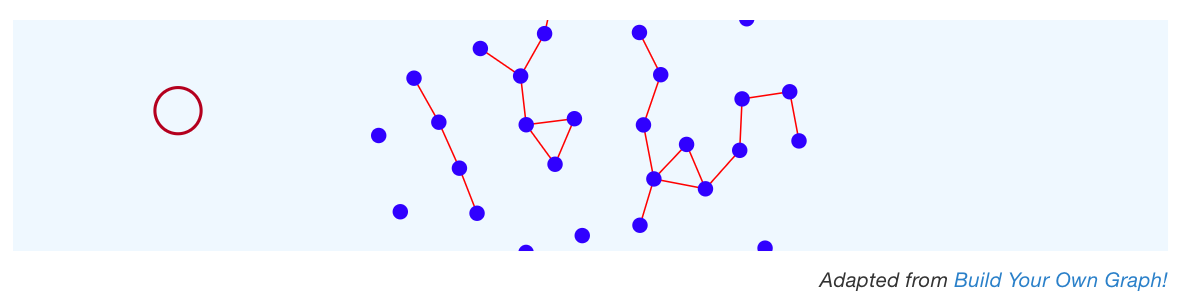
\includegraphics[width=1\linewidth]{images/pdfbook/buildyourowngraph}

This guide serves as a companion text to Scott Murray's \href{https://www.amazon.com/Interactive-Data-Visualization-Web-Introduction/dp/1491921285/}{\emph{Interactive Data Visualization for the Web, 2nd edition}}--henceforth \emph{IDVW2}--a required text for GR5702. Be sure to get the second edition, which is a comprehensive update to D3 version 4. The first edition uses D3 version 3, which is not compatible. (The current version of D3 is actually v6. However, since differences between v4 and v5/v6 are minimal, unless otherwise indicated in this guide, the code in \emph{IDVW2} will work with either.)

We rely on the text heavily but also deviate from it in several ways. \emph{IDVW2} is written for graphics designers not data science students so the pain points are somewhat different.

D3 is a JavaScript library, not a standalone language, so any time we refer to D3 we really mean D3/JavaScript, though it is not necessary to know JavaScript well before beginning; we will learn as we go. Most of the JavaScript we use is covered in \emph{IDVW2}, though we also use some newer JavaScript options from ES5 and ES6, such as \texttt{.map()}, \texttt{.filter()}, arrow functions and template literals, that make coding easier (and more like R!)\footnote{Ok, they're not actually that new, but it takes a while for new JavaScript to catch on, mainly due to concern with maintaining compatibility with older browsers. Since D3 itself is not compatible with very old browsers, and since we can't focus on everything at once, we are not going to concern ourselves with browser compatibility. If you are interested in this, \href{https://caniuse.com}{caniuse.com} is very helpful for looking up what works where.} We use different examples, though you are strongly encouraged to study \href{https://github.com/alignedleft/d3-book/releases}{Murray's code examples} in addition to reading the text. Particularly through the first half, we don't follow the text in order, so always refer to this guide first which will direct you to the pages of the text that you should read.

This is very much a work-in-progress so please \href{https://github.com/jtr13/d3book/issues}{submit issues} on GitHub to provide feedback and edit or add text by submitting pull requests. (Click the icon at the top of each page to get started. More \href{https://edav.info/contribute.html\#step-2-click-the-edit-button}{detailed instructions} are available on edav.info. If you would just like to view the source code, click the icon.)

\hypertarget{workflow}{%
\section{Workflow}\label{workflow}}

A big hurdle to learning a new language is just getting setup. Often authors forget to mention what your programming environment should look like, what should be open on the screen. I will try not to do that and be as clear as possible so you know where you should be entering the code in the pages that follow. This task is somewhat complicated by the fact that we will be using a variety of workflow options. This section will serve as a reference guide; future sections will link back here as appropriate.

All of our workflows require Google Chrome, so if you don't have it already, \href{https://www.google.com/chrome/}{download and install it}.

\hypertarget{javascript-console}{%
\subsection{JavaScript Console}\label{javascript-console}}

With this workflow we will open a web page--either online or local--in Chrome and \href{https://developers.google.com/web/tools/chrome-devtools/console/javascript}{run JavaScript in the Console}. To view the Console, open Chrome DevTools by clicking \emph{View, Developer, JavaScript Console} if you have a menu bar in Chrome, using a keyboard shortcut (Mac: option+command+j; Windows, Linux, Chrome OS: control+shift+J), or employing another one of the \href{https://developers.google.com/web/tools/chrome-devtools/open}{many options} for doing so. The Console is one piece of a suite of tools available in the browser.

With the DevTools open, your screen will look like this:

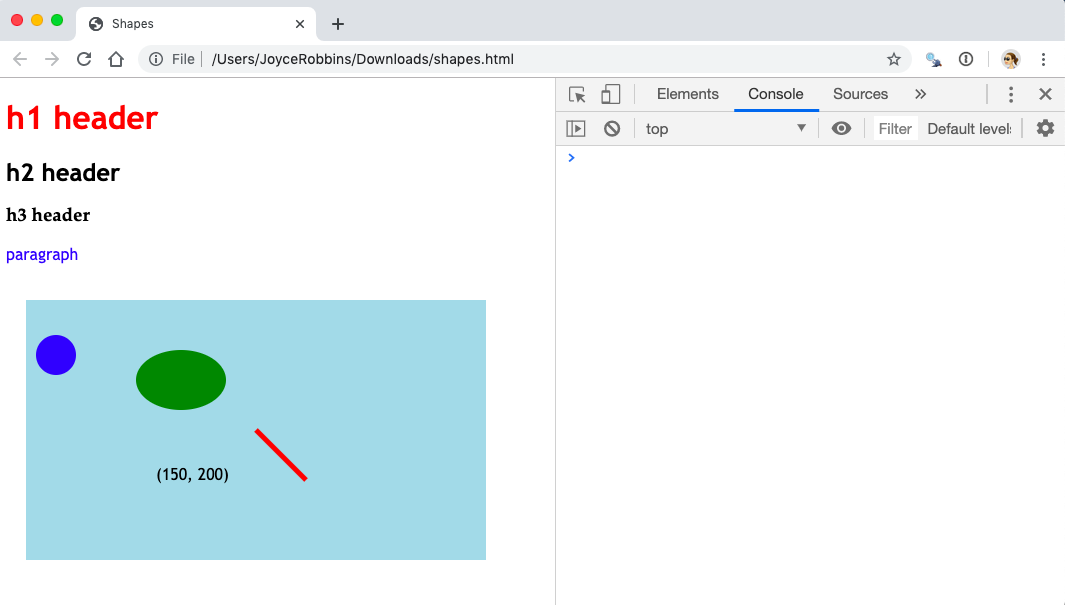
\includegraphics[width=1\linewidth]{images/console}

The next chapter, \href{jump.html}{Jump in the deep end}, employs this workflow.

\hypertarget{this-book-in-the-console}{%
\subsection{This book in the Console}\label{this-book-in-the-console}}

If you're not reading the \texttt{.pdf} version, you can open DevTools on this very page. This is very convenient because not only to you not have to leave this book to practice D3, you can copy code blocks and paste them in the Console. In addition to opening DevTools (see above), close the side bar by clicking on the icon above to give yourself more screen space.

Let's try it out.

\begin{quote}
\emph{Open the JavaScript Console}
\end{quote}


\includegraphics[width=0.33\linewidth]{images/pdfbook/svg1}

Scroll so that both the blue rectangle above and the code chunk below are visible on your screen. Toggle the sidebar, open the Console, and then move the mouse onto the code block so the icon appears. Click on it to copy the code, paste it in the Console, and then press return.

\begin{Shaded}
\begin{Highlighting}[]
\NormalTok{d3}\OperatorTok{.}\FunctionTok{select}\NormalTok{(}\StringTok{"svg\#demo"}\NormalTok{)}
  \OperatorTok{.}\FunctionTok{append}\NormalTok{(}\StringTok{"circle"}\NormalTok{)}
    \OperatorTok{.}\FunctionTok{attr}\NormalTok{(}\StringTok{"cx"}\OperatorTok{,} \StringTok{"{-}25"}\NormalTok{)              }
    \OperatorTok{.}\FunctionTok{attr}\NormalTok{(}\StringTok{"cy"}\OperatorTok{,} \StringTok{"100"}\NormalTok{)}
    \OperatorTok{.}\FunctionTok{attr}\NormalTok{(}\StringTok{"r"}\OperatorTok{,} \StringTok{"20"}\NormalTok{)}
    \OperatorTok{.}\FunctionTok{attr}\NormalTok{(}\StringTok{"fill"}\OperatorTok{,} \StringTok{"red"}\NormalTok{)}
  \OperatorTok{.}\FunctionTok{transition}\NormalTok{()}
  \OperatorTok{.}\FunctionTok{duration}\NormalTok{(}\DecValTok{3000}\NormalTok{)}
    \OperatorTok{.}\FunctionTok{attr}\NormalTok{(}\StringTok{"cx"}\OperatorTok{,} \StringTok{"325"}\NormalTok{)}
  \OperatorTok{.}\FunctionTok{remove}\NormalTok{()}\OperatorTok{;}
\end{Highlighting}
\end{Shaded}

Pretty neat.

\hypertarget{text-editor}{%
\subsection{Text editor}\label{text-editor}}

This is a very basic local setup in which the same \texttt{.html} is open both in a text editor (if you don't want to stray too far from home, use RStudio) and in a web browser (we will use Chrome), each on one half of your screen. The workflow is: make changes to the file in the text editor, save the changes and then refresh the page in the browser to see the updates. Keyboard shortcuts for saving and refreshing (on the Mac, command-s and command-r respectively) are very helpful.

Let's try an example:

Download a copy of \texttt{shapes.html} by opening \href{https://raw.githubusercontent.com/jtr13/d3book/master/code/shapes.html}{this page} and clicking \emph{File, Save Page As\ldots{}} Open the file in a text editor of your choice on one half of your screen. On the other half of your screen open the same file in Chrome. As you make changes to the \texttt{.html} file, save the file and then refresh the browser to see the effects.

Your screen should look like this:

\begin{center}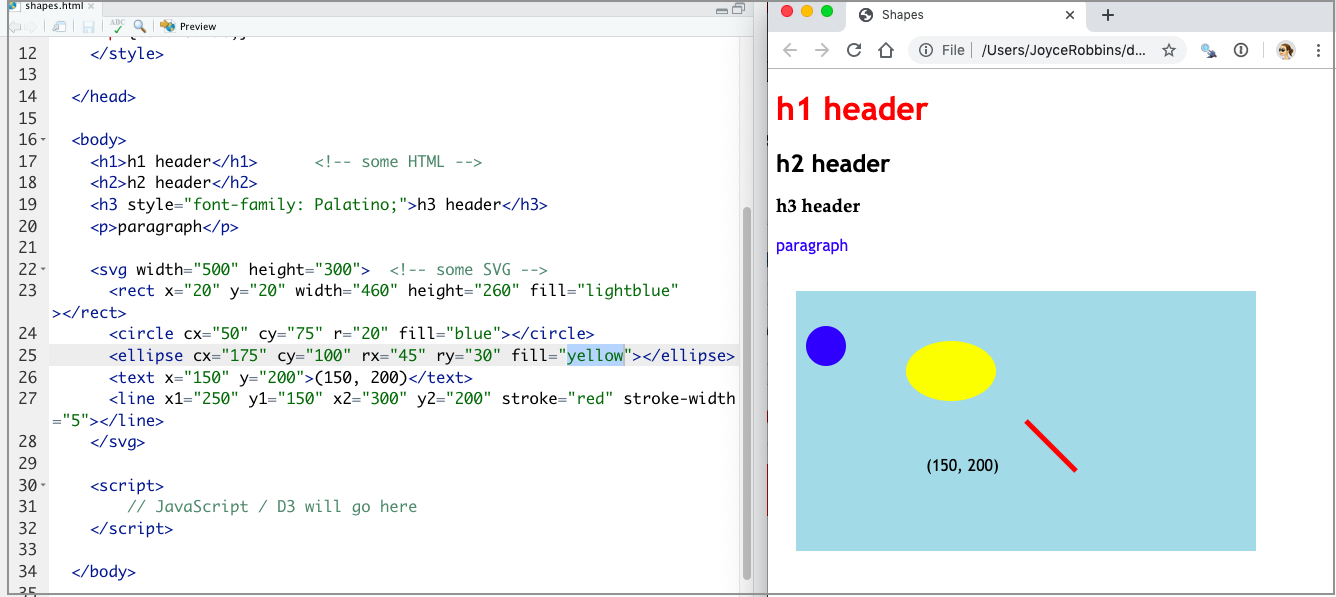
\includegraphics[width=0.8\linewidth]{images/editor_chrome} \end{center}

\hypertarget{jump}{%
\chapter{\texorpdfstring{Jump in the deep end }{Jump in the deep end }}\label{jump}}

Let's skip the explanations and start coding in D3 right now. Why? So you can see the benefits and know what you're working toward when you get stuck in the weeds. Then we'll go back and start learning step by step. In this chapter we will work in the JavaScript Console (\href{index.html\#javascript-console}{help}).

\hypertarget{get-ready}{%
\section{\texorpdfstring{Get ready }{Get ready }}\label{get-ready}}

\begin{enumerate}
\def\labelenumi{\arabic{enumi}.}
\item
  If you don't have it, \href{https://www.google.com/chrome/}{install the Chrome browser}.
\item
  Download a copy of \texttt{shapes.html} by opening the following page and then saving with \emph{File, Save Page As\ldots{}}: \href{https://raw.githubusercontent.com/jtr13/d3book/master/code/shapes.html}{\texttt{shapes.html}}. (Or download a zip of the whole repo. Clicking \href{https://github.com/jtr13/d3book/archive/master.zip}{here} will start the download. Or fork and clone the \href{https://github.com/jtr13/d3book}{repo}).
\item
  If Chrome is your default browser, open \texttt{shapes.html} by double clicking it. Otherwise, open it with \emph{File, Open File\ldots{}} in Chrome.
\end{enumerate}

\hypertarget{elements-tab}{%
\section{\texorpdfstring{Elements tab }{Elements tab }}\label{elements-tab}}

\begin{enumerate}
\def\labelenumi{\arabic{enumi}.}
\item
  Open Chrome DevTools (\href{index.html\#javascript-console}{help}).
\item
  Hover the mouse over various elements in the \texttt{\textless{}body\textgreater{}\ ...\ \textless{}/body\textgreater{}} section. Observe the highlighted sections in the rendered web page on the left of the screen. Click on the mini black triangles to the left of the \texttt{\textless{}body\textgreater{}} and \texttt{\textless{}svg\textgreater{}} tags if needed to open these sections of the DOM tree. Your screen should look like this:
\end{enumerate}

\begin{center}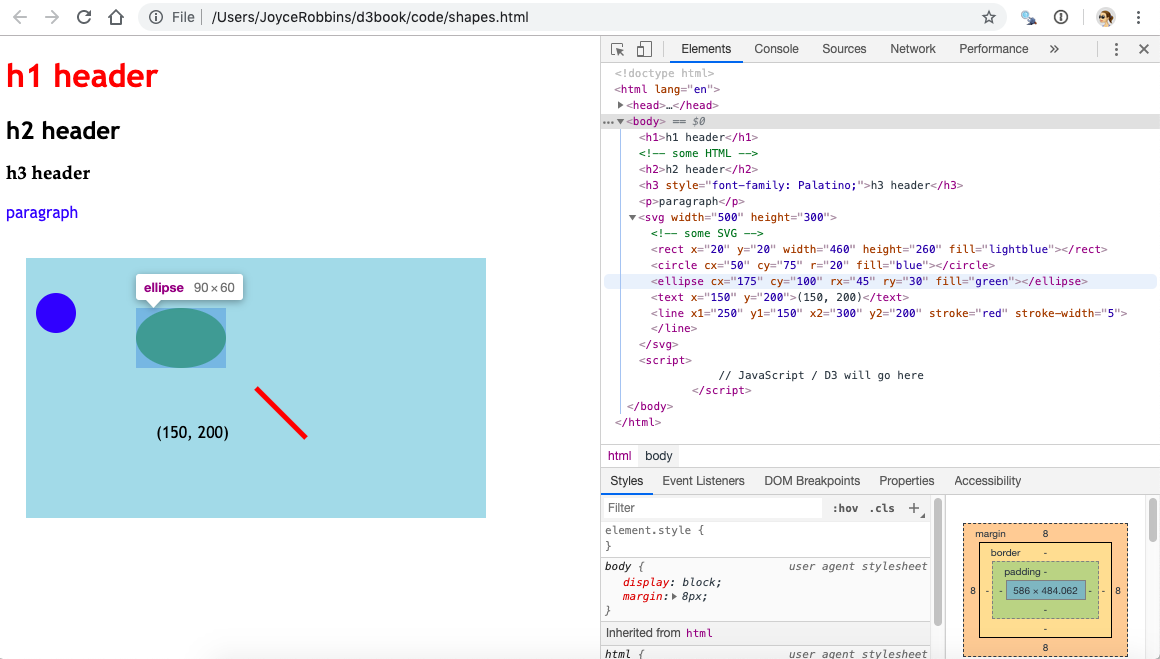
\includegraphics[width=0.8\linewidth]{images/elements} \end{center}

\begin{enumerate}
\def\labelenumi{\arabic{enumi}.}
\setcounter{enumi}{2}
\tightlist
\item
  Now try the reverse: right click on elements on the web page, choose ``Inspect'' and see what is highlighted in the Elements pane. Get comfortable with the connection between the code on the right and the rendered elements on the left.
\end{enumerate}

\hypertarget{console-tab}{%
\section{\texorpdfstring{Console tab }{Console tab }}\label{console-tab}}

\begin{enumerate}
\def\labelenumi{\arabic{enumi}.}
\tightlist
\item
  Switch to the Console tab, next to the Elements tab. Let's practice running some code. Note that the code is unrelated to the \texttt{shapes.html} web page that we have open.
\end{enumerate}

\begin{quote}
\emph{We will spend a lot of time in the Console since it's interactive -- think R console. Eventually we will switch to including JavaScript/D3 in \texttt{.html} or \texttt{.js} files and use the Console only for testing things out or debugging.}
\end{quote}

\begin{enumerate}
\def\labelenumi{\arabic{enumi}.}
\setcounter{enumi}{1}
\tightlist
\item
  Type the following lines of code at the prompt (\texttt{\textgreater{}}), press enter after each line--that is, after the semicolon (\texttt{;})--and see what happens:
\end{enumerate}

\begin{Shaded}
\begin{Highlighting}[]
\DecValTok{3} \OperatorTok{+} \DecValTok{4}\OperatorTok{;}
    
\StringTok{"3"} \OperatorTok{+} \StringTok{"4"}\OperatorTok{;}

\NormalTok{ x }\OperatorTok{=}\NormalTok{ [}\DecValTok{1}\OperatorTok{,} \DecValTok{2}\OperatorTok{,} \DecValTok{3}\NormalTok{]}\OperatorTok{;}
    
\NormalTok{x[}\DecValTok{1}\NormalTok{]}\OperatorTok{;}
    
\NormalTok{x }\OperatorTok{+} \DecValTok{1}\OperatorTok{;}
    
\NormalTok{y }\OperatorTok{=}\NormalTok{ \{}\DataTypeTok{a}\OperatorTok{:} \DecValTok{3}\OperatorTok{,} \DataTypeTok{b}\OperatorTok{:} \DecValTok{4}\NormalTok{\}}\OperatorTok{;}
    
\NormalTok{y[}\StringTok{"b"}\NormalTok{]}\OperatorTok{;}
\end{Highlighting}
\end{Shaded}

\hypertarget{modify-elements}{%
\section{\texorpdfstring{Modify elements }{Modify elements }}\label{modify-elements}}

\begin{enumerate}
\def\labelenumi{\arabic{enumi}.}
\item
  Now we'll start using D3 to manipulate elements on the page. Try the following, by entering one line at a time in the Console as before:

\begin{Shaded}
\begin{Highlighting}[]
\NormalTok{d3}\OperatorTok{.}\FunctionTok{select}\NormalTok{(}\StringTok{"circle"}\NormalTok{)}\OperatorTok{.}\FunctionTok{attr}\NormalTok{(}\StringTok{"cx"}\OperatorTok{,} \StringTok{"200"}\NormalTok{)}\OperatorTok{;}

\NormalTok{d3}\OperatorTok{.}\FunctionTok{select}\NormalTok{(}\StringTok{"circle"}\NormalTok{)}\OperatorTok{.}\FunctionTok{attr}\NormalTok{(}\StringTok{"cx"}\OperatorTok{,} \StringTok{"500"}\NormalTok{)}\OperatorTok{;}

\NormalTok{d3}\OperatorTok{.}\FunctionTok{select}\NormalTok{(}\StringTok{"circle"}\NormalTok{)}\OperatorTok{.}\FunctionTok{attr}\NormalTok{(}\StringTok{"cx"}\OperatorTok{,} \StringTok{"100"}\NormalTok{)}\OperatorTok{;}

\NormalTok{d3}\OperatorTok{.}\FunctionTok{select}\NormalTok{(}\StringTok{"circle"}\NormalTok{)}\OperatorTok{.}\FunctionTok{attr}\NormalTok{(}\StringTok{"r"}\OperatorTok{,} \StringTok{"30"}\NormalTok{)}\OperatorTok{;}

\NormalTok{d3}\OperatorTok{.}\FunctionTok{select}\NormalTok{(}\StringTok{"circle"}\NormalTok{)}\OperatorTok{.}\FunctionTok{attr}\NormalTok{(}\StringTok{"r"}\OperatorTok{,} \StringTok{"130"}\NormalTok{)}\OperatorTok{;}

\NormalTok{d3}\OperatorTok{.}\FunctionTok{select}\NormalTok{(}\StringTok{"circle"}\NormalTok{)}\OperatorTok{.}\FunctionTok{attr}\NormalTok{(}\StringTok{"r"}\OperatorTok{,} \StringTok{"3"}\NormalTok{)}\OperatorTok{;}

\NormalTok{d3}\OperatorTok{.}\FunctionTok{select}\NormalTok{(}\StringTok{"circle"}\NormalTok{)}\OperatorTok{.}\FunctionTok{attr}\NormalTok{(}\StringTok{"fill"}\OperatorTok{,} \StringTok{"red"}\NormalTok{)}\OperatorTok{;}

\NormalTok{d3}\OperatorTok{.}\FunctionTok{select}\NormalTok{(}\StringTok{"circle"}\NormalTok{)}\OperatorTok{.}\FunctionTok{attr}\NormalTok{(}\StringTok{"fill"}\OperatorTok{,} \StringTok{"aliceblue"}\NormalTok{)}\OperatorTok{;}

\NormalTok{d3}\OperatorTok{.}\FunctionTok{select}\NormalTok{(}\StringTok{"circle"}\NormalTok{)}\OperatorTok{.}\FunctionTok{attr}\NormalTok{(}\StringTok{"fill"}\OperatorTok{,} \StringTok{"lightseagreen"}\NormalTok{)}\OperatorTok{;}
\end{Highlighting}
\end{Shaded}
\end{enumerate}

\begin{quote}
\emph{Note that ``select'' and ``attr'' are separate operations chained together with ``.'' -- think pipe (\%\textgreater\%) operator.}
\end{quote}

\begin{enumerate}
\def\labelenumi{\arabic{enumi}.}
\setcounter{enumi}{1}
\item
  Refresh the page. What happened?
\item
  Go to Elements. Look at the value of the \texttt{y1} attribute of the SVG \texttt{\textless{}line\textgreater{}} element. Go back to the Console and enter the following:

\begin{Shaded}
\begin{Highlighting}[]
\NormalTok{d3}\OperatorTok{.}\FunctionTok{select}\NormalTok{(}\StringTok{"line"}\NormalTok{)}\OperatorTok{.}\FunctionTok{attr}\NormalTok{(}\StringTok{"y1"}\OperatorTok{,} \StringTok{"10"}\NormalTok{)}\OperatorTok{;}
\end{Highlighting}
\end{Shaded}
\item
  Switch back to Elements and observe. What happened?
\item
  Stay in Elements and refresh the page. What happened to \texttt{y1}?
\item
  Return to the Console to make style changes to the HTML elements:

\begin{Shaded}
\begin{Highlighting}[]
\NormalTok{d3}\OperatorTok{.}\FunctionTok{select}\NormalTok{(}\StringTok{"h1"}\NormalTok{)}\OperatorTok{.}\FunctionTok{style}\NormalTok{(}\StringTok{"color"}\OperatorTok{,} \StringTok{"purple"}\NormalTok{)}\OperatorTok{;}

\NormalTok{d3}\OperatorTok{.}\FunctionTok{select}\NormalTok{(}\StringTok{"h2"}\NormalTok{)}\OperatorTok{.}\FunctionTok{style}\NormalTok{(}\StringTok{"font{-}size"}\OperatorTok{,} \StringTok{"50px"}\NormalTok{)}\OperatorTok{;}

\NormalTok{d3}\OperatorTok{.}\FunctionTok{select}\NormalTok{(}\StringTok{"h2"}\NormalTok{)}\OperatorTok{.}\FunctionTok{style}\NormalTok{(}\StringTok{"font{-}family"}\OperatorTok{,} \StringTok{"Impact"}\NormalTok{)}\OperatorTok{;}
\end{Highlighting}
\end{Shaded}
\end{enumerate}

\hypertarget{add-transitions}{%
\section{\texorpdfstring{Add transitions }{Add transitions }}\label{add-transitions}}

\begin{enumerate}
\def\labelenumi{\arabic{enumi}.}
\item
  Try these:

\begin{Shaded}
\begin{Highlighting}[]
\NormalTok{d3}\OperatorTok{.}\FunctionTok{select}\NormalTok{(}\StringTok{"circle"}\NormalTok{)}\OperatorTok{.}\FunctionTok{transition}\NormalTok{()}\OperatorTok{.}\FunctionTok{duration}\NormalTok{(}\DecValTok{2000}\NormalTok{)}\OperatorTok{.}\FunctionTok{attr}\NormalTok{(}\StringTok{"cx"}\OperatorTok{,} \StringTok{"400"}\NormalTok{)}\OperatorTok{;}

\NormalTok{d3}\OperatorTok{.}\FunctionTok{select}\NormalTok{(}\StringTok{"ellipse"}\NormalTok{)}\OperatorTok{.}\FunctionTok{transition}\NormalTok{()}\OperatorTok{.}\FunctionTok{duration}\NormalTok{(}\DecValTok{2000}\NormalTok{)}\OperatorTok{.}\FunctionTok{attr}\NormalTok{(}\StringTok{"transform"}\OperatorTok{,} \StringTok{"translate (400, 400)"}\NormalTok{)}\OperatorTok{;}

\NormalTok{d3}\OperatorTok{.}\FunctionTok{select}\NormalTok{(}\StringTok{"line"}\NormalTok{)}\OperatorTok{.}\FunctionTok{transition}\NormalTok{()}\OperatorTok{.}\FunctionTok{duration}\NormalTok{(}\DecValTok{2000}\NormalTok{)}\OperatorTok{.}\FunctionTok{attr}\NormalTok{(}\StringTok{"x1"}\OperatorTok{,} \StringTok{"400"}\NormalTok{)}\OperatorTok{;}

\NormalTok{d3}\OperatorTok{.}\FunctionTok{select}\NormalTok{(}\StringTok{"line"}\NormalTok{)}\OperatorTok{.}\FunctionTok{transition}\NormalTok{()}\OperatorTok{.}\FunctionTok{duration}\NormalTok{(}\DecValTok{2000}\NormalTok{)}\OperatorTok{.}\FunctionTok{attr}\NormalTok{(}\StringTok{"y1"}\OperatorTok{,} \StringTok{"250"}\NormalTok{)}\OperatorTok{;}

\NormalTok{d3}\OperatorTok{.}\FunctionTok{select}\NormalTok{(}\StringTok{"p"}\NormalTok{)}\OperatorTok{.}\FunctionTok{transition}\NormalTok{()}\OperatorTok{.}\FunctionTok{duration}\NormalTok{(}\DecValTok{2000}\NormalTok{)}\OperatorTok{.}\FunctionTok{style}\NormalTok{(}\StringTok{"font{-}size"}\OperatorTok{,} \StringTok{"72px"}\NormalTok{)}\OperatorTok{;}
\end{Highlighting}
\end{Shaded}
\item
  Experiment with more transitions.
\end{enumerate}

\hypertarget{add-interactivity}{%
\section{\texorpdfstring{Add interactivity }{Add interactivity }}\label{add-interactivity}}

\begin{enumerate}
\def\labelenumi{\arabic{enumi}.}
\item
  Set up a function to turn the fill color to yellow:

\begin{Shaded}
\begin{Highlighting}[]
\KeywordTok{function} \FunctionTok{goyellow}\NormalTok{() \{d3}\OperatorTok{.}\FunctionTok{select}\NormalTok{(}\KeywordTok{this}\NormalTok{)}\OperatorTok{.}\FunctionTok{attr}\NormalTok{(}\StringTok{"fill"}\OperatorTok{,} \StringTok{"yellow"}\NormalTok{)\}}\OperatorTok{;}
\end{Highlighting}
\end{Shaded}
\item
  Add an event listener to the circle that will be trigger a call to \texttt{goyellow()} on a mouseover:

\begin{Shaded}
\begin{Highlighting}[]
\NormalTok{d3}\OperatorTok{.}\FunctionTok{select}\NormalTok{(}\StringTok{"circle"}\NormalTok{)}\OperatorTok{.}\FunctionTok{on}\NormalTok{(}\StringTok{"mouseover"}\OperatorTok{,}\NormalTok{ goyellow)}\OperatorTok{;}
\end{Highlighting}
\end{Shaded}
\item
  Test it out.
\item
  Add the same event listener to the ellipse. Test it out.
\item
  Create a function \texttt{goblue()} that changes the fill color to blue.
\item
  Add event listeners to the circle and ellipse that will trigger a call to \texttt{goblue()} on a \emph{mouseout}. Test out your code.
\item
  Try out a click event. (Note the use of an anonymous function.)

\begin{Shaded}
\begin{Highlighting}[]
\NormalTok{d3}\OperatorTok{.}\FunctionTok{select}\NormalTok{(}\StringTok{"line"}\NormalTok{)}\OperatorTok{.}\FunctionTok{on}\NormalTok{(}\StringTok{"click"}\OperatorTok{,} \KeywordTok{function}\NormalTok{()}
\NormalTok{  \{d3}\OperatorTok{.}\FunctionTok{select}\NormalTok{(}\KeywordTok{this}\NormalTok{)}\OperatorTok{.}\FunctionTok{attr}\NormalTok{(}\StringTok{"stroke{-}width"}\OperatorTok{,} \StringTok{"10"}\NormalTok{)}\OperatorTok{;}\NormalTok{\})}\OperatorTok{;}
\end{Highlighting}
\end{Shaded}
\item
  Try another click event. What's happening?

  \textbf{v6}

\begin{Shaded}
\begin{Highlighting}[]
\NormalTok{d3}\OperatorTok{.}\FunctionTok{select}\NormalTok{(}\StringTok{"svg"}\NormalTok{)}\OperatorTok{.}\FunctionTok{on}\NormalTok{(}\StringTok{"click"}\OperatorTok{,} \KeywordTok{function}\NormalTok{(}\BuiltInTok{event}\NormalTok{)}
\NormalTok{  \{d3}\OperatorTok{.}\FunctionTok{select}\NormalTok{(}\StringTok{"text"}\NormalTok{)}\OperatorTok{.}\FunctionTok{text}\NormalTok{(}\VerbatimStringTok{\textasciigrave{}(}\SpecialCharTok{$\{}\NormalTok{d3}\OperatorTok{.}\FunctionTok{pointer}\NormalTok{(}\BuiltInTok{event}\NormalTok{)}\SpecialCharTok{\}}\VerbatimStringTok{)\textasciigrave{}}\NormalTok{)\})}\OperatorTok{;}
\end{Highlighting}
\end{Shaded}

  \textbf{v5}

\begin{Shaded}
\begin{Highlighting}[]
\NormalTok{d3}\OperatorTok{.}\FunctionTok{select}\NormalTok{(}\StringTok{"svg"}\NormalTok{)}\OperatorTok{.}\FunctionTok{on}\NormalTok{(}\StringTok{"click"}\OperatorTok{,} \KeywordTok{function}\NormalTok{()}
\NormalTok{  \{d3}\OperatorTok{.}\FunctionTok{select}\NormalTok{(}\StringTok{"text"}\NormalTok{)}\OperatorTok{.}\FunctionTok{text}\NormalTok{(}\VerbatimStringTok{\textasciigrave{}(}\SpecialCharTok{$\{}\NormalTok{d3}\OperatorTok{.}\FunctionTok{mouse}\NormalTok{(}\KeywordTok{this}\NormalTok{)}\SpecialCharTok{\}}\VerbatimStringTok{)\textasciigrave{}}\NormalTok{)\})}\OperatorTok{;}
\end{Highlighting}
\end{Shaded}
\end{enumerate}

\hypertarget{web}{%
\chapter{\texorpdfstring{Web tech }{Web tech }}\label{web}}

Read \emph{IDVW2}, Chapter 3: Technology Fundamentals

\emph{There is a lot of material in this chapter. It is worth making the effort to learn it now and start D3 with a solid foundation of elementary HTML/CSS/SVG/JavaScript.}

Here we examine \texttt{shapes.html} from Chapter 1 to see how the various technologies are combined into a single document.

\hypertarget{html}{%
\section{\texorpdfstring{HTML }{HTML }}\label{html}}

Note that \texttt{shapes.html} has an HyperText Markup Language or \texttt{.html} extension; HTML in fact provides the structure for the document. It has a \texttt{\textless{}head\textgreater{}} and \texttt{\textless{}body\textgreater{}} section.

In the \texttt{\textless{}head\textgreater{}} section we use \texttt{\textless{}script\textgreater{}} tags to link to the D3 library:

\begin{Shaded}
\begin{Highlighting}[]
\OperatorTok{\textless{}}\NormalTok{script src}\OperatorTok{=}\StringTok{"https://d3js.org/d3.v6.js"}\OperatorTok{\textgreater{}\textless{}/}\NormalTok{script}\OperatorTok{\textgreater{}}
\end{Highlighting}
\end{Shaded}

HTML content is enclosed between opening an closing \textbf{tags} such as \texttt{\textless{}h1\textgreater{}} and \texttt{\textless{}/h1\textgreater{}}.

HTML class and ID \textbf{attributes} are included inside the opening tags:

\texttt{\textless{}h1\ class="myclass"\ id="myid"\textgreater{}This\ is\ an\ h1\ header.\textless{}/h1\textgreater{}}

\hypertarget{css}{%
\section{\texorpdfstring{CSS }{CSS }}\label{css}}

CSS (Cascading Style Sheets) is used for styling web pages, and more importantly for our purposes, selecting elements on a page or in a graphic. We will generally work with internal style sheets since it's simpler when starting out to have everything in one document. External style sheets, however, are generally the preferred method for web design.

\hypertarget{internal-style-sheet}{%
\subsection{Internal style sheet}\label{internal-style-sheet}}

\texttt{shapes.html} has an \emph{internal style sheet}: CSS style information appears in the \texttt{\textless{}head\textgreater{}} section marked off with \texttt{\textless{}style\textgreater{}} tags:

\begin{Shaded}
\begin{Highlighting}[]
\OperatorTok{\textless{}}\NormalTok{style type}\OperatorTok{=}\StringTok{"text/css"}\OperatorTok{\textgreater{}}
\NormalTok{    h1 \{}\DataTypeTok{color}\OperatorTok{:}\NormalTok{red}\OperatorTok{;}\NormalTok{\}     }\CommentTok{/* CSS styling */}
\NormalTok{    p \{}\DataTypeTok{color}\OperatorTok{:}\NormalTok{blue}\OperatorTok{;}\NormalTok{\}}
\OperatorTok{\textless{}/}\NormalTok{style}\OperatorTok{\textgreater{}}
\end{Highlighting}
\end{Shaded}

Here we specify that all HTML \texttt{\textless{}h1\textgreater{}} headers should be red and all HTML paragraphs \texttt{\textless{}p\textgreater{}} should be blue. This is an example of an \emph{internal style sheet}. Later we will consider alternatives: \emph{external style sheets} and \emph{inline styling}.

Styling for coder designed classes is also specified in this section. For example, we could style a ``formal'' class as such:

\begin{Shaded}
\begin{Highlighting}[]
\OperatorTok{\textless{}}\NormalTok{style type}\OperatorTok{=}\StringTok{"text/css"}\OperatorTok{\textgreater{}}
    \OperatorTok{.}\AttributeTok{formal}\NormalTok{ \{}\DataTypeTok{color}\OperatorTok{:}\NormalTok{ red}\OperatorTok{;}        
\NormalTok{        font}\OperatorTok{{-}}\DataTypeTok{size}\OperatorTok{:}\NormalTok{ 30px}\OperatorTok{;}
\NormalTok{        font}\OperatorTok{{-}}\DataTypeTok{family}\OperatorTok{:}\NormalTok{ Lucida Calligraphy}\OperatorTok{;}
\NormalTok{        \}   }
\OperatorTok{\textless{}/}\NormalTok{style}\OperatorTok{\textgreater{}}
\end{Highlighting}
\end{Shaded}

Note that classes are defined by the ``.'' before the name.

\hypertarget{external-style-sheets}{%
\subsection{External style sheets}\label{external-style-sheets}}

External style sheets are \texttt{.css} files that contain styling information and are linked to with a \texttt{\textless{}link\textgreater{}} tag in the \texttt{\textless{}head\textgreater{}} section of an HTML document:

\begin{Shaded}
\begin{Highlighting}[]
\OperatorTok{\textless{}}\NormalTok{head}\OperatorTok{\textgreater{}}
    \OperatorTok{\textless{}}\NormalTok{link rel}\OperatorTok{=}\StringTok{"stylesheet"}\NormalTok{ href}\OperatorTok{=}\StringTok{"style.css"}\OperatorTok{\textgreater{}}
\OperatorTok{\textless{}/}\NormalTok{head}\OperatorTok{\textgreater{}}
\end{Highlighting}
\end{Shaded}

External style sheets are the preferred way of styling as they can easily be modified without changing the web page; in fact, the motivation for CSS came from a desire in the early days of the internet to separate styling from content.

Developers have the option now of choosing premade themes, which are shared through external style sheets. They can be quite complex. The \href{https://github.com/thomaspark/bootswatch/blob/master/docs/4/minty/bootstrap.css}{\texttt{.css} file} for the ~Minty~ theme from Bootswatch, for example, contains over 10,000 lines.

\href{http://www.csszengarden.com/}{CSS Zen Garden} demonstrates the power of external style sheets: the same HTML document takes on very different looks depending on the stylesheet to which it is linked.

\hypertarget{inline-styling}{%
\subsection{Inline styling}\label{inline-styling}}

With inline styling, styling is added to each tag individually:

\begin{verbatim}
<span style="color: white; background-color: fuchsia; font-family: impact; 
      font-size: 24px; border-style: solid; border-color: limegreen; 
      border-width: 3px">
      Styled inline
</span>
\end{verbatim}

{Styled inline}

This is how early web pages were styled. To take a step back in time, use developer tools to view the source code for the main page of \href{http://www.dolekemp96.org/main.htm}{www.dolekemp96.org}, an old web site that has been maintained for historical purposes. As you can see, it's a tedious way of writing content, which internal and external style sheets eliminate.

Although you will not be adding inline styling manually, you will notice that when we select elements and change the styling with D3, the modifications are made inline. In other words, we do not make changes to the elements directly, not via a style sheet.

\hypertarget{svg}{%
\section{\texorpdfstring{SVG }{SVG }}\label{svg}}

SVG (Scalable Vector Graphics) is a human readable graphics format that facilitates manipulation of individual elements. You may be familiar with \texttt{.svg} files. Here we have SVG graphics within \texttt{\textless{}svg\textgreater{}} tags in the \texttt{\textless{}body\textgreater{}} section of the HTML document:

\begin{Shaded}
\begin{Highlighting}[]
\OperatorTok{\textless{}}\NormalTok{svg width}\OperatorTok{=}\StringTok{"500"}\NormalTok{ height}\OperatorTok{=}\StringTok{"300"}\OperatorTok{\textgreater{}}  \OperatorTok{\textless{}!{-}{-}}\NormalTok{ some SVG }\OperatorTok{{-}{-}\textgreater{}}
    \OperatorTok{\textless{}}\NormalTok{rect x}\OperatorTok{=}\StringTok{"20"}\NormalTok{ y}\OperatorTok{=}\StringTok{"20"}\NormalTok{ width}\OperatorTok{=}\StringTok{"460"}\NormalTok{ height}\OperatorTok{=}\StringTok{"260"}\NormalTok{ fill}\OperatorTok{=}\StringTok{"lightblue"}\OperatorTok{\textgreater{}\textless{}/}\NormalTok{rect}\OperatorTok{\textgreater{}}
    \OperatorTok{\textless{}}\NormalTok{circle cx}\OperatorTok{=}\StringTok{"50"}\NormalTok{ cy}\OperatorTok{=}\StringTok{"75"}\NormalTok{ r}\OperatorTok{=}\StringTok{"20"}\NormalTok{ fill}\OperatorTok{=}\StringTok{"blue"}\OperatorTok{\textgreater{}\textless{}/}\NormalTok{circle}\OperatorTok{\textgreater{}}
    \OperatorTok{\textless{}}\NormalTok{ellipse cx}\OperatorTok{=}\StringTok{"175"}\NormalTok{ cy}\OperatorTok{=}\StringTok{"100"}\NormalTok{ rx}\OperatorTok{=}\StringTok{"45"}\NormalTok{ ry}\OperatorTok{=}\StringTok{"30"}\NormalTok{ fill}\OperatorTok{=}\StringTok{"green"}\OperatorTok{\textgreater{}\textless{}/}\NormalTok{ellipse}\OperatorTok{\textgreater{}}
    \OperatorTok{\textless{}}\NormalTok{text x}\OperatorTok{=}\StringTok{"150"}\NormalTok{ y}\OperatorTok{=}\StringTok{"200"}\OperatorTok{\textgreater{}}\NormalTok{(}\DecValTok{150}\OperatorTok{,} \DecValTok{200}\NormalTok{)}\OperatorTok{\textless{}/}\NormalTok{text}\OperatorTok{\textgreater{}}
    \OperatorTok{\textless{}}\NormalTok{line x1}\OperatorTok{=}\StringTok{"250"}\NormalTok{ y1}\OperatorTok{=}\StringTok{"150"}\NormalTok{ x2}\OperatorTok{=}\StringTok{"300"}\NormalTok{ y2}\OperatorTok{=}\StringTok{"200"}\NormalTok{ stroke}\OperatorTok{=}\StringTok{"red"}\NormalTok{ stroke}\OperatorTok{{-}}\NormalTok{width}\OperatorTok{=}\StringTok{"5"}\OperatorTok{\textgreater{}\textless{}/}\NormalTok{line}\OperatorTok{\textgreater{}}
\OperatorTok{\textless{}/}\NormalTok{svg}\OperatorTok{\textgreater{}}
\end{Highlighting}
\end{Shaded}

Rendered:

`

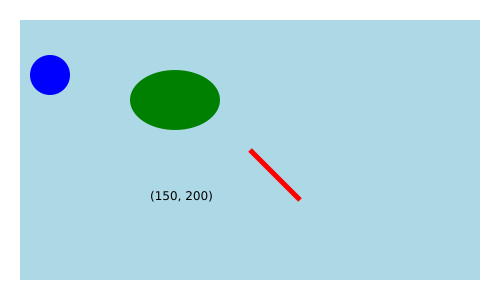
\includegraphics[width=0.5\linewidth]{images/shapessvg}

(150, 200)

There are very few SVG tags that you'll need to know, and once we get going with D3, you will not have to code any SVG manually. It is worth doing a little to become familiar with the format and in particular to get used to the new location of the origin.

\hypertarget{javascript}{%
\section{\texorpdfstring{JavaScript }{JavaScript }}\label{javascript}}

JavaScript is the most common language for making web pages interactive. Code is executed when pages are opened or refreshed. So far we have run JavaScript in the Console, but have not included it in the web page itself. When we do so, it will be between \texttt{\textless{}script\textgreater{}} tags in the \texttt{\textless{}body\textgreater{}} section of the HTML document, or in a separate \texttt{.js} file.

We will learn JavaScript on an as-needed basis. In terms of data, we will begin with simple arrays:

\texttt{var\ x\ =\ {[}3,\ 5,\ 1,\ 6,\ 7{]}}

In the \href{just-enough-js.html}{Just Enough JS} chapter, we cover more complex data structures and some methods for data manipulation.

\href{https://javascript.info}{javascript.info} is an excellent resource for expanding your knowledge beyond the basics.

\hypertarget{d3}{%
\section{\texorpdfstring{D3 }{D3 }}\label{d3}}

D3 (Data Driven Documents) is a JavaScript library well suited to interactive graphics. As such, it is also included between \texttt{\textless{}script\textgreater{}} tags in the \texttt{\textless{}body\textgreater{}} section. For D3 to work, you must link to the D3 library in the \texttt{\textless{}head\textgreater{}} section of the document.

There seems to be a misconception that D3 is a high level language. It is not. You will be working on the pixel level to create graphics, including drawing your own axes and doing other things that you're not used to doing if you've been working in R or Python.

\begin{quote}
\emph{On the bright side, after D3, you will gain a new appreciation for base R graphics. You will write code such as \texttt{plot(iris\$Sepal.Length,\ iris\$Sepal.Width,\ pch\ =\ 16,\ col\ =\ iris\$Species,\ las\ =\ 1,\ xlab\ =\ "Sepal.Length",\ ylab\ =\ "Sepal.Width")} and think: wow, there are axes! Amazing!}
\end{quote}

It is legitimate to ask why you need to know D3 as a data scientist. Many if not most of you will not be coding in JavaScript from the ground up in your future careers. However, it's a great way to learn how interactive graphics work under the hood, and will give you a solid foundation which you can draw on to tweak visualizations that you build with high level tools such as \href{https://plot.ly/}{Plotly}.

\hypertarget{html-tree}{%
\section{\texorpdfstring{HTML tree }{HTML tree }}\label{html-tree}}

While \texttt{shapes.html} appears as a single consistent document, it is actually comprised of multiple languages. HTML, CSS, and SVG are already there, and we will be adding JavaScript / D3 soon.

\begin{center}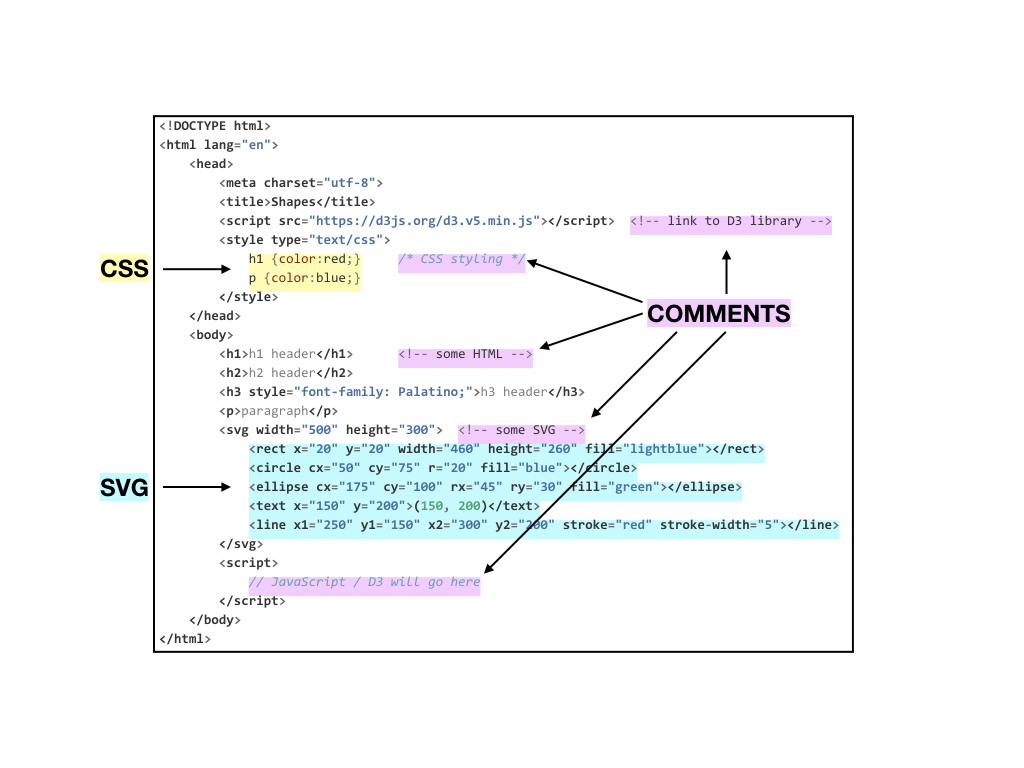
\includegraphics[width=1\linewidth]{images/shapes} \end{center}

Of note:

\begin{itemize}
\item
  An HTML document is composed of lines or sections set off with tags. In particular \texttt{\textless{}style\textgreater{}\ ...\ \textless{}/style\textgreater{}}, \texttt{\textless{}svg\textgreater{}\ ...\ \textless{}/svg\textgreater{}}, and \texttt{\textless{}script\textgreater{}\ ...\ \textless{}/script\textgreater{}} indicate the inclusion of CSS, SVG, and JavaScript/D3 respectively.
\item
  For D3 to work, you must link to a D3 library. To link to the online version, copy and paste the \texttt{\textless{}script\textgreater{}} line from \url{https://d3js.org}. Alternatively, you can also download a copy from the same site and reference your local copy with:

\begin{Shaded}
\begin{Highlighting}[]
\OperatorTok{\textless{}}\NormalTok{script src}\OperatorTok{=}\StringTok{"d3.js"}\OperatorTok{\textgreater{}\textless{}/}\NormalTok{script}\OperatorTok{\textgreater{}}
\end{Highlighting}
\end{Shaded}
\item
  There are two main sections. The \texttt{\textless{}head\textgreater{}} section contains the \emph{title}, \emph{link to D3 library}, and \emph{internal CSS}. The \texttt{\textless{}body\textgreater{}} section contains HTML elements (\texttt{\textless{}h1\textgreater{}}, \texttt{\textless{}p\textgreater{}}, etc.), SVGs (between \texttt{\textless{}svg\textgreater{}}/\texttt{\textless{}/svg\textgreater{}}tags) and JavaScript/D3 scripts (between \texttt{\textless{}script\textgreater{}}/\texttt{\textless{}script\textgreater{}}tags).
\end{itemize}

\begin{quote}
\emph{Do not assume that if it works that it is correct; today's browsers can be very forgiving.}
\end{quote}

\begin{itemize}
\item
  Comment syntax varies with language:

  \begin{itemize}
  \item
    \texttt{\textless{}!-\/-\ single\ or\ multiline\ HTML\ or\ SVG\ comment\ -\/-\textgreater{}}
  \item
    \texttt{/*\ single\ or\ multiline\ CSS\ comment\ */}
  \item
    \texttt{//\ single\ line\ JavaScript\ comment}
  \item
    \texttt{/*\ JavaScript} \texttt{multiline\ comment\ */}
  \end{itemize}
\end{itemize}

\hypertarget{exercise-shapes}{%
\section{Exercise : shapes}\label{exercise-shapes}}

Download a copy of \texttt{shapes.html} by opening \href{https://raw.githubusercontent.com/jtr13/d3book/master/code/shapes.html}{this page} and clicking \emph{File, Save Page As\ldots{}} Set yourself up to work locally in a text editor \href{index.html\#text-editor}{help}. (Developer Tools should not be open; we will not be using the Console.)

\begin{enumerate}
\def\labelenumi{\arabic{enumi}.}
\item
  Add an additional circle to the svg.
\item
  Add styling to the internal style sheet to style circles.
\item
  Add two additional paragraphs use the \texttt{\textless{}p\textgreater{}} tag.
\item
  Add an ID attribute to one of the circles.
\item
  Add a class attribute to two of the \texttt{\textless{}p\textgreater{}} tags.
\item
  Use the internal style sheet to style paragraphs of the class you created in 5.
\item
  Adjust additional elements as desired.
\end{enumerate}

\protect\hyperlink{web-tech-shapes}{}

\hypertarget{d3console}{%
\chapter{\texorpdfstring{D3 in the Console }{D3 in the Console }}\label{d3console}}

Read \emph{IDVW2}, Chapter 6: Drawing with Data. Skip pp.~89-96 as we will not be drawing bar charts with the \texttt{div}approach.

\hypertarget{selections}{%
\section{\texorpdfstring{Selections }{Selections }}\label{selections}}

\hypertarget{select-by-tag}{%
\subsection{Select by tag}\label{select-by-tag}}

The ability to select elements on a page is key to being able to manipulate them. \texttt{d3.select()} will select the first match; \texttt{d3.selectAll()} will select all matches.

\begin{Shaded}
\begin{Highlighting}[]
\NormalTok{d3}\OperatorTok{.}\FunctionTok{select}\NormalTok{(}\StringTok{"svg"}\NormalTok{)}\OperatorTok{.}\FunctionTok{select}\NormalTok{(}\StringTok{"circle"}\NormalTok{)}\OperatorTok{;}
\end{Highlighting}
\end{Shaded}

selects the first circle in the order in which circles appear in the \texttt{\textless{}svg\textgreater{}} grouping. If there were more than one circle we could select them all with:

\begin{Shaded}
\begin{Highlighting}[]
\NormalTok{d3}\OperatorTok{.}\FunctionTok{select}\NormalTok{(}\StringTok{"svg"}\NormalTok{)}\OperatorTok{.}\FunctionTok{selectAll}\NormalTok{(}\StringTok{"circle"}\NormalTok{)}\OperatorTok{;}
\end{Highlighting}
\end{Shaded}

We can select HTML elements by tag in the same way:

\begin{Shaded}
\begin{Highlighting}[]
\NormalTok{d3}\OperatorTok{.}\FunctionTok{select}\NormalTok{(}\StringTok{"body"}\NormalTok{)}\OperatorTok{.}\FunctionTok{select}\NormalTok{(}\StringTok{"h1"}\NormalTok{)}\OperatorTok{;}
\NormalTok{d3}\OperatorTok{.}\FunctionTok{select}\NormalTok{(}\StringTok{"body"}\NormalTok{)}\OperatorTok{.}\FunctionTok{selectAll}\NormalTok{(}\StringTok{"h1"}\NormalTok{)}\OperatorTok{;}
\end{Highlighting}
\end{Shaded}

\hypertarget{select-by-class}{%
\subsection{Select by class}\label{select-by-class}}

Classes are selected by adding a ``.'' before the class name:

\begin{Shaded}
\begin{Highlighting}[]
\NormalTok{d3}\OperatorTok{.}\FunctionTok{select}\NormalTok{(}\StringTok{"svg"}\NormalTok{)}\OperatorTok{.}\FunctionTok{selectAll}\NormalTok{(}\StringTok{"circle.apple"}\NormalTok{)}
\end{Highlighting}
\end{Shaded}

This provides one method of selecting a certain collection of elements of the same type.

\hypertarget{select-by-id}{%
\subsection{Select by ID}\label{select-by-id}}

IDs differ from classes in that they are unique identifies. IDs are selected by adding a ``\#'' before the ID:

\begin{Shaded}
\begin{Highlighting}[]
\NormalTok{d3}\OperatorTok{.}\FunctionTok{select}\NormalTok{(}\StringTok{"svg"}\NormalTok{)}\OperatorTok{.}\FunctionTok{select}\NormalTok{(}\StringTok{"circle\#henry"}\NormalTok{)}\OperatorTok{;}
\end{Highlighting}
\end{Shaded}

\hypertarget{store-selections}{%
\subsection{Store selections}\label{store-selections}}

It is often helpful to store selections for later use. Here we store the svg selection in \texttt{mysvg}:

\begin{Shaded}
\begin{Highlighting}[]
\KeywordTok{var}\NormalTok{ mysvg }\OperatorTok{=}\NormalTok{ d3}\OperatorTok{.}\FunctionTok{select}\NormalTok{(}\StringTok{"svg"}\NormalTok{)}\OperatorTok{;}
\end{Highlighting}
\end{Shaded}

\begin{quote}
\emph{The JavaScript community is moving toward using \texttt{let} and \texttt{const} instead of \texttt{var}; we, however, will stick with \texttt{var} to be consistent with }IDVW2\emph{. Of course you're welcome to use \texttt{const} and \texttt{let} instead, and if so, may find these articles helpful: \href{https://madhatted.com/2016/1/25/let-it-be}{Let It Be - How to declare JavaScript variables} and \href{https://mathiasbynens.be/notes/es6-const}{ES2015 const is not about immutability}.}
\end{quote}

Store circle selection in a variable:

\begin{Shaded}
\begin{Highlighting}[]
\KeywordTok{var}\NormalTok{ svg }\OperatorTok{=}\NormalTok{ d3}\OperatorTok{.}\FunctionTok{select}\NormalTok{(}\StringTok{"svg"}\NormalTok{)}\OperatorTok{;}

\KeywordTok{var}\NormalTok{ circ }\OperatorTok{=}\NormalTok{ svg}\OperatorTok{.}\FunctionTok{selectAll}\NormalTok{(}\StringTok{"circle"}\NormalTok{)}\OperatorTok{;}
\end{Highlighting}
\end{Shaded}

\hypertarget{modify-existing-elements}{%
\section{\texorpdfstring{Modify existing elements }{Modify existing elements }}\label{modify-existing-elements}}

Try out the code in this section with a downloaded copy of \href{https://raw.githubusercontent.com/jtr13/d3book/master/code/five_green_circles.html}{five\_green\_circles.html} opened in Chrome and the Console visible.

\hypertarget{modify-attributes}{%
\subsection{Modify attributes}\label{modify-attributes}}

\href{https://github.com/d3/d3-selection/blob/v1.4.0/README.md\#selection_attr}{link to get or set attribute API}

\begin{Shaded}
\begin{Highlighting}[]
\NormalTok{d3}\OperatorTok{.}\FunctionTok{select}\NormalTok{(}\StringTok{"circle"}\NormalTok{)}\OperatorTok{.}\FunctionTok{attr}\NormalTok{(}\StringTok{"r"}\NormalTok{)}\OperatorTok{;}           \CommentTok{// see radius}

\NormalTok{d3}\OperatorTok{.}\FunctionTok{select}\NormalTok{(}\StringTok{"circle"}\NormalTok{)}\OperatorTok{.}\FunctionTok{attr}\NormalTok{(}\StringTok{"r"}\OperatorTok{,} \StringTok{"10"}\NormalTok{)}\OperatorTok{;}     \CommentTok{// set radius to 10}
\end{Highlighting}
\end{Shaded}

\hypertarget{modify-styles}{%
\subsection{Modify styles}\label{modify-styles}}

\href{https://github.com/d3/d3-selection/blob/v1.4.0/README.md\#selection_style}{link to get or set style API}

\begin{Shaded}
\begin{Highlighting}[]
\NormalTok{d3}\OperatorTok{.}\FunctionTok{select}\NormalTok{(}\StringTok{"h1"}\NormalTok{)}\OperatorTok{.}\FunctionTok{style}\NormalTok{(}\StringTok{"color"}\NormalTok{)}\OperatorTok{;}

\NormalTok{d3}\OperatorTok{.}\FunctionTok{select}\NormalTok{(}\StringTok{"h1"}\NormalTok{)}\OperatorTok{.}\FunctionTok{style}\NormalTok{(}\StringTok{"color"}\OperatorTok{,} \StringTok{"blue"}\NormalTok{)}\OperatorTok{;}
\end{Highlighting}
\end{Shaded}

\begin{quote}
\emph{It is often difficult to remember whether to use \texttt{.attr()} or \texttt{.style()} In general, properties such as position on the SVG, class, and ID are }attributes\emph{, while decorative properties such as color, font, font size, etc. are }styles\emph{. However, in some cases, you can use either. For example, the following both make the circle blue:}
\end{quote}

\begin{Shaded}
\begin{Highlighting}[]
\NormalTok{d3}\OperatorTok{.}\FunctionTok{select}\NormalTok{(}\StringTok{"circle"}\NormalTok{)}\OperatorTok{.}\FunctionTok{attr}\NormalTok{(}\StringTok{"fill"}\OperatorTok{,} \StringTok{"blue"}\NormalTok{)}\OperatorTok{;}

\NormalTok{d3}\OperatorTok{.}\FunctionTok{select}\NormalTok{(}\StringTok{"circle"}\NormalTok{)}\OperatorTok{.}\FunctionTok{style}\NormalTok{(}\StringTok{"fill"}\OperatorTok{,} \StringTok{"blue"}\NormalTok{)}\OperatorTok{;}
\end{Highlighting}
\end{Shaded}

\emph{The first will add a \texttt{fill="blue"} attribute to the \texttt{\textless{}circle\textgreater{}} tag, while the latter will add \texttt{style="fill:\ blue;"}. All is well and good until you find yourself with both in the same tag, in which case the \texttt{style} property will take precedence. The bottom line: don't mix the two options because it can cause problems.}

\begin{quote}
\emph{To further complicate matters, \texttt{.style()} is just shorthand for \texttt{.attr("style",\ "...")} so the following are in fact equivalent:}
\end{quote}

\begin{Shaded}
\begin{Highlighting}[]
\NormalTok{d3}\OperatorTok{.}\FunctionTok{select}\NormalTok{(}\StringTok{"circle"}\NormalTok{)}\OperatorTok{.}\FunctionTok{style}\NormalTok{(}\StringTok{"fill"}\OperatorTok{,} \StringTok{"blue"}\NormalTok{)}\OperatorTok{;}

\NormalTok{d3}\OperatorTok{.}\FunctionTok{select}\NormalTok{(}\StringTok{"circle"}\NormalTok{)}\OperatorTok{.}\FunctionTok{attr}\NormalTok{(}\StringTok{"style"}\OperatorTok{,} \StringTok{"fill: blue;"}\NormalTok{)}\OperatorTok{;}
\end{Highlighting}
\end{Shaded}

\emph{In other words, style is an attribute!}

\hypertarget{modify-text}{%
\subsection{Modify text}\label{modify-text}}

This section is interactive. Hover over code as directed to observe effects.

\hypertarget{html-text}{%
\subsubsection*{HTML text}\label{html-text}}
\addcontentsline{toc}{subsubsection}{HTML text}

\begin{Shaded}
\begin{Highlighting}[]
\KeywordTok{\textless{}p}\OtherTok{ id=}\StringTok{"typo"}\OtherTok{ class=}\StringTok{"fancy"}\KeywordTok{\textgreater{}}\NormalTok{Manhatten}\KeywordTok{\textless{}/p\textgreater{}}
\end{Highlighting}
\end{Shaded}

Manhatten

Hover to execute this code (and fix the typo):

\hypertarget{fixtypo}{}
\begin{Shaded}
\begin{Highlighting}[]
\NormalTok{d3}\OperatorTok{.}\FunctionTok{select}\NormalTok{(}\StringTok{"\#typo"}\NormalTok{)}\OperatorTok{.}\FunctionTok{text}\NormalTok{(}\StringTok{"Manhattan"}\NormalTok{)}\OperatorTok{;}
\end{Highlighting}
\end{Shaded}

\hypertarget{svg-text}{%
\subsubsection*{SVG text}\label{svg-text}}
\addcontentsline{toc}{subsubsection}{SVG text}

\begin{Shaded}
\begin{Highlighting}[]
\KeywordTok{\textless{}svg}\OtherTok{ width=}\StringTok{"500"}\OtherTok{ height=}\StringTok{"100"}\KeywordTok{\textgreater{}}
  \KeywordTok{\textless{}rect}\OtherTok{ width=}\StringTok{"500"}\OtherTok{ height=}\StringTok{"100"}\OtherTok{ fill=}\StringTok{"\#326EA4"}\KeywordTok{\textgreater{}\textless{}/rect\textgreater{}}
  \KeywordTok{\textless{}text}\OtherTok{ id=}\StringTok{"svgtypo"}\OtherTok{ x=}\StringTok{"50"}\OtherTok{ y=}\StringTok{"70"}\OtherTok{ fill=}\StringTok{"white"}\OtherTok{ font{-}weight=}\StringTok{"bold"}\OtherTok{ font{-}size=}\StringTok{"40px"}\KeywordTok{\textgreater{}}
\NormalTok{     Web scrapping is fun.}\KeywordTok{\textless{}/text\textgreater{}}
\KeywordTok{\textless{}/svg\textgreater{}}  
\end{Highlighting}
\end{Shaded}

Hover on this SVG to execute the code below it (and fix the typo):

Web scrapping is fun.

\hypertarget{fixsvgtypo}{}
\begin{Shaded}
\begin{Highlighting}[]
\NormalTok{d3}\OperatorTok{.}\FunctionTok{select}\NormalTok{(}\StringTok{"\#svgtypo"}\NormalTok{)}\OperatorTok{.}\FunctionTok{text}\NormalTok{(}\StringTok{"Web scraping is fun."}\NormalTok{)}\OperatorTok{;}
\end{Highlighting}
\end{Shaded}

\begin{quote}
\emph{The SVG \texttt{\textless{}text\textgreater{}} tag can be tricky. It differs from HTML text tags (\texttt{\textless{}p\textgreater{},\ \textless{}h1\textgreater{},\ \textless{}h2\textgreater{},} etc.) in that it has \texttt{x} and \texttt{y} attributes that allow you to position text on an SVG canvas. Unlike HTML, the fill attribute controls the color of the text. Compare:}
\end{quote}

\begin{Shaded}
\begin{Highlighting}[]
\NormalTok{d3}\OperatorTok{.}\FunctionTok{select}\NormalTok{(}\StringTok{"p"}\NormalTok{)}\OperatorTok{.}\FunctionTok{style}\NormalTok{(}\StringTok{"color"}\OperatorTok{,} \StringTok{"red"}\NormalTok{)}\OperatorTok{;}   \CommentTok{// HTML}

\NormalTok{d3}\OperatorTok{.}\FunctionTok{select}\NormalTok{(}\StringTok{"text"}\NormalTok{)}\OperatorTok{.}\FunctionTok{attr}\NormalTok{(}\StringTok{"fill"}\OperatorTok{,} \StringTok{"red"}\NormalTok{)}\OperatorTok{;}  \CommentTok{// SVG}
\end{Highlighting}
\end{Shaded}

\hypertarget{move-svg-text}{%
\subsection{Move SVG text}\label{move-svg-text}}

\begin{Shaded}
\begin{Highlighting}[]
\KeywordTok{\textless{}svg}\OtherTok{ width=}\StringTok{"600"}\OtherTok{ height=}\StringTok{"100"}\KeywordTok{\textgreater{}}
  \KeywordTok{\textless{}rect}\OtherTok{ width=}\StringTok{"600"}\OtherTok{ height=}\StringTok{"100"}\OtherTok{ fill=}\StringTok{"\#326EA4"}\KeywordTok{\textgreater{}\textless{}/rect\textgreater{}}
  \KeywordTok{\textless{}text}\OtherTok{ id=}\StringTok{"moveleft"}\OtherTok{ x=}\StringTok{"200"}\OtherTok{ y=}\StringTok{"70"}\OtherTok{ fill=}\StringTok{"white"}\OtherTok{ font{-}weight=}\StringTok{"bold"}\OtherTok{ font{-}size=}\StringTok{"40px"}\KeywordTok{\textgreater{}}
\NormalTok{      I want to move left.}\KeywordTok{\textless{}/text\textgreater{}}
\KeywordTok{\textless{}/svg\textgreater{}}  
\end{Highlighting}
\end{Shaded}

Hover on this SVG to execute the code below it:

I want to move left.

\hypertarget{move}{}
\begin{Shaded}
\begin{Highlighting}[]
\NormalTok{d3}\OperatorTok{.}\FunctionTok{select}\NormalTok{(}\StringTok{"\#moveleft"}\NormalTok{)}\OperatorTok{.}\FunctionTok{attr}\NormalTok{(}\StringTok{"x"}\OperatorTok{,} \StringTok{"20"}\NormalTok{)}\OperatorTok{.}\FunctionTok{text}\NormalTok{(}\StringTok{"Thanks, now I\textquotesingle{}m happy!"}\NormalTok{)}\OperatorTok{;}
\end{Highlighting}
\end{Shaded}

\hypertarget{add-elements}{%
\section{\texorpdfstring{Add elements }{Add elements }}\label{add-elements}}

\hypertarget{html-1}{%
\subsection{HTML}\label{html-1}}

Continue trying out code with \texttt{five\_green\_circles.html} open in Chrome.

The following adds a \texttt{\textless{}p\textgreater{}} tag but doesn't change how the page looks, since there's no text associated with it.

\begin{Shaded}
\begin{Highlighting}[]
\NormalTok{d3}\OperatorTok{.}\FunctionTok{select}\NormalTok{(}\StringTok{"body"}\NormalTok{)}\OperatorTok{.}\FunctionTok{append}\NormalTok{(}\StringTok{"p"}\NormalTok{)}\OperatorTok{;}
\end{Highlighting}
\end{Shaded}

To add text, use \texttt{.text()}:

\begin{Shaded}
\begin{Highlighting}[]
\NormalTok{d3}\OperatorTok{.}\FunctionTok{select}\NormalTok{(}\StringTok{"body"}\NormalTok{)}\OperatorTok{.}\FunctionTok{append}\NormalTok{(}\StringTok{"p"}\NormalTok{)}\OperatorTok{.}\FunctionTok{text}\NormalTok{(}\StringTok{"This is a complete sentence."}\NormalTok{)}\OperatorTok{;}
\end{Highlighting}
\end{Shaded}

\begin{quote}
\emph{To debug adding an element, go to the Elements tab to see what was added and where. If an element is in the wrong place in the HTML tree, it will not be visible.}
\end{quote}

\hypertarget{svg-1}{%
\subsection{SVG}\label{svg-1}}

Likewise, here we add a \texttt{\textless{}circle\textgreater{}} to the \texttt{\textless{}svg\textgreater{}}, but we can't see it since it has no attributes.

\begin{Shaded}
\begin{Highlighting}[]
\NormalTok{d3}\OperatorTok{.}\FunctionTok{select}\NormalTok{(}\StringTok{"svg"}\NormalTok{)}\OperatorTok{.}\FunctionTok{append}\NormalTok{(}\StringTok{"circle"}\NormalTok{)}\OperatorTok{;}
\end{Highlighting}
\end{Shaded}

Adding attributes will create visible circles:

\begin{Shaded}
\begin{Highlighting}[]
\NormalTok{d3}\OperatorTok{.}\FunctionTok{select}\NormalTok{(}\StringTok{"svg"}\NormalTok{)}\OperatorTok{.}\FunctionTok{append}\NormalTok{(}\StringTok{"rect"}\NormalTok{)}\OperatorTok{.}\FunctionTok{attr}\NormalTok{(}\StringTok{"x"}\OperatorTok{,} \StringTok{"0"}\NormalTok{)}\OperatorTok{.}\FunctionTok{attr}\NormalTok{(}\StringTok{"y"}\OperatorTok{,} \StringTok{"0"}\NormalTok{)}
    \OperatorTok{.}\FunctionTok{attr}\NormalTok{(}\StringTok{"width"}\OperatorTok{,} \StringTok{"500"}\NormalTok{)}\OperatorTok{.}\FunctionTok{attr}\NormalTok{(}\StringTok{"height"}\OperatorTok{,} \StringTok{"400"}\NormalTok{)}\OperatorTok{.}\FunctionTok{attr}\NormalTok{(}\StringTok{"fill"}\OperatorTok{,} \StringTok{"lightblue"}\NormalTok{)}\OperatorTok{;}
    
\NormalTok{d3}\OperatorTok{.}\FunctionTok{select}\NormalTok{(}\StringTok{"svg"}\NormalTok{)}\OperatorTok{.}\FunctionTok{append}\NormalTok{(}\StringTok{"circle"}\NormalTok{)}\OperatorTok{.}\FunctionTok{attr}\NormalTok{(}\StringTok{"cx"}\OperatorTok{,} \StringTok{"200"}\NormalTok{)}
    \OperatorTok{.}\FunctionTok{attr}\NormalTok{(}\StringTok{"cy"}\OperatorTok{,} \StringTok{"100"}\NormalTok{)}\OperatorTok{.}\FunctionTok{attr}\NormalTok{(}\StringTok{"r"}\OperatorTok{,} \StringTok{"25"}\NormalTok{)}\OperatorTok{.}\FunctionTok{attr}\NormalTok{(}\StringTok{"fill"}\OperatorTok{,} \StringTok{"orange"}\NormalTok{)}\OperatorTok{;}
    
\NormalTok{d3}\OperatorTok{.}\FunctionTok{select}\NormalTok{(}\StringTok{"svg"}\NormalTok{)}\OperatorTok{.}\FunctionTok{append}\NormalTok{(}\StringTok{"circle"}\NormalTok{)}\OperatorTok{.}\FunctionTok{attr}\NormalTok{(}\StringTok{"cx"}\OperatorTok{,} \StringTok{"300"}\NormalTok{)}
    \OperatorTok{.}\FunctionTok{attr}\NormalTok{(}\StringTok{"cy"}\OperatorTok{,} \StringTok{"150"}\NormalTok{)}\OperatorTok{.}\FunctionTok{attr}\NormalTok{(}\StringTok{"r"}\OperatorTok{,} \StringTok{"25"}\NormalTok{)}\OperatorTok{.}\FunctionTok{attr}\NormalTok{(}\StringTok{"fill"}\OperatorTok{,} \StringTok{"red"}\NormalTok{)}\OperatorTok{;}  
\end{Highlighting}
\end{Shaded}

We can use a saved selection to assist in creating a new element:

(\emph{IDVW2}, pp.~97-98)

\begin{Shaded}
\begin{Highlighting}[]
\NormalTok{mysvg }\OperatorTok{=}\NormalTok{ d3}\OperatorTok{.}\FunctionTok{select}\NormalTok{(}\StringTok{"svg"}\NormalTok{)}\OperatorTok{;}

\NormalTok{mysvg}\OperatorTok{.}\FunctionTok{append}\NormalTok{(}\StringTok{"circle"}\NormalTok{)}\OperatorTok{.}\FunctionTok{attr}\NormalTok{(}\StringTok{"cx"}\OperatorTok{,} \StringTok{"250"}\NormalTok{)}\OperatorTok{.}\FunctionTok{attr}\NormalTok{(}\StringTok{"cy"}\OperatorTok{,} \StringTok{"250"}\NormalTok{)}\OperatorTok{.}\FunctionTok{attr}\NormalTok{(}\StringTok{"r"}\OperatorTok{,} \StringTok{"50"}\NormalTok{)}
  \OperatorTok{.}\FunctionTok{attr}\NormalTok{(}\StringTok{"fill"}\OperatorTok{,} \StringTok{"red"}\NormalTok{)}\OperatorTok{;}
\end{Highlighting}
\end{Shaded}

\hypertarget{remove-elements}{%
\section{\texorpdfstring{Remove elements }{Remove elements }}\label{remove-elements}}

These methods will remove matching elements in order, starting with the first find in the document.

\hypertarget{html-2}{%
\subsection{HTML}\label{html-2}}

\begin{Shaded}
\begin{Highlighting}[]
\NormalTok{d3}\OperatorTok{.}\FunctionTok{select}\NormalTok{(}\StringTok{"p"}\NormalTok{)}\OperatorTok{.}\FunctionTok{remove}\NormalTok{()}\OperatorTok{;}
\end{Highlighting}
\end{Shaded}

\hypertarget{svg-2}{%
\subsection{SVG}\label{svg-2}}

\begin{Shaded}
\begin{Highlighting}[]
\NormalTok{d3}\OperatorTok{.}\FunctionTok{select}\NormalTok{(}\StringTok{"svg"}\NormalTok{)}\OperatorTok{.}\FunctionTok{select}\NormalTok{(}\StringTok{"circle"}\NormalTok{)}\OperatorTok{.}\FunctionTok{remove}\NormalTok{()}\OperatorTok{;}

\NormalTok{d3}\OperatorTok{.}\FunctionTok{select}\NormalTok{(}\StringTok{"svg"}\NormalTok{)}\OperatorTok{.}\FunctionTok{selectAll}\NormalTok{(}\StringTok{"circle"}\NormalTok{)}\OperatorTok{.}\FunctionTok{remove}\NormalTok{()}\OperatorTok{;}
\end{Highlighting}
\end{Shaded}

\hypertarget{exercise-green-circles}{%
\section{Exercise : green circles}\label{exercise-green-circles}}

Download and open a fresh copy of \href{https://raw.githubusercontent.com/jtr13/d3book/master/code/five_green_circles.html}{five\_green\_circles.html} in Chrome. Open Developer Tools open and do the following in the Console with D3:

\begin{enumerate}
\def\labelenumi{\arabic{enumi}.}
\item
  Select the circle with ID ``henry'' and make it blue.
\item
  Select all circles of ``apple'' class make them red.
\item
  Select the first circle and add an orange border (``stroke''), and stroke width (``stroke-width'') of 5.
\item
  Select all circles of ``apple'' class and move them to the middle of the svg.
\end{enumerate}

\protect\hyperlink{d3-in-the-console-green-circles}{}

\hypertarget{exercise-blue-circles}{%
\section{\texorpdfstring{Exercise : blue circles}{Exercise  : blue circles}}\label{exercise-blue-circles}}

Download and open a fresh copy of \href{https://raw.githubusercontent.com/jtr13/d3book/master/code/six_blue_circles.html}{six\_blue\_circles.html} in Chrome. Open Developer Tools and execute Steps 1-4 one at a time in the Console. After Step 4, refresh the page to go back to Step 1 if so desired. (You do not need to create a loop as in the visual.)

\begin{quote}
\emph{This exercise is provided as a challenge. It's fine to skip this exercise and move on to the next section.}
\end{quote}

\begin{enumerate}
\def\labelenumi{\arabic{enumi}.}
\item
  Move all the circles to the right.
\item
  Move them back to the left \emph{and} change their color.
\item
  In a text editor, add an id to the third circle in \texttt{six\_blue\_circles.html}, save the file, and then in the Console, move only that circle to the right.
\item
  Move all the circles to the middle of the screen, \emph{then} move them all to the same location.
\end{enumerate}

\protect\hyperlink{d3-in-the-console-blue-circles}{}

\hypertarget{bind-data-finally}{%
\section{\texorpdfstring{Bind data\ldots{} \emph{finally!} }{Bind data\ldots{} finally! }}\label{bind-data-finally}}

(\emph{IDVW2}, pp.~98-108)

To follow along with the code in this section, download and open \href{https://raw.githubusercontent.com/jtr13/d3book/master/code/six_blue_circles.html}{six\_blue\_circles.html}.

Bind data:

\begin{Shaded}
\begin{Highlighting}[]
\NormalTok{d3}\OperatorTok{.}\FunctionTok{select}\NormalTok{(}\StringTok{"svg"}\NormalTok{)}\OperatorTok{.}\FunctionTok{selectAll}\NormalTok{(}\StringTok{"circle"}\NormalTok{)}\OperatorTok{.}\FunctionTok{data}\NormalTok{([}\DecValTok{90}\OperatorTok{,} \DecValTok{230}\OperatorTok{,} \DecValTok{140}\OperatorTok{,} \DecValTok{75}\OperatorTok{,} \DecValTok{180}\OperatorTok{,} \DecValTok{25}\NormalTok{])}\OperatorTok{;}
\end{Highlighting}
\end{Shaded}

Check data binding:

\begin{Shaded}
\begin{Highlighting}[]
\NormalTok{d3}\OperatorTok{.}\FunctionTok{select}\NormalTok{(}\StringTok{"svg"}\NormalTok{)}\OperatorTok{.}\FunctionTok{selectAll}\NormalTok{(}\StringTok{"circle"}\NormalTok{)}\OperatorTok{.}\FunctionTok{data}\NormalTok{()}\OperatorTok{;}
\end{Highlighting}
\end{Shaded}

Set x-coordinate of each circle to data value using arrow function:

\begin{Shaded}
\begin{Highlighting}[]
\NormalTok{d3}\OperatorTok{.}\FunctionTok{select}\NormalTok{(}\StringTok{"svg"}\NormalTok{)}\OperatorTok{.}\FunctionTok{selectAll}\NormalTok{(}\StringTok{"circle"}\NormalTok{)}\OperatorTok{.}\FunctionTok{attr}\NormalTok{(}\StringTok{"cx"}\OperatorTok{,}\NormalTok{ d }\KeywordTok{=\textgreater{}}\NormalTok{ d)}\OperatorTok{;}
\end{Highlighting}
\end{Shaded}

Set x-coordinate of each circle to data value with a JavaScript function:

\begin{Shaded}
\begin{Highlighting}[]
\NormalTok{d3}\OperatorTok{.}\FunctionTok{select}\NormalTok{(}\StringTok{"svg"}\NormalTok{)}\OperatorTok{.}\FunctionTok{selectAll}\NormalTok{(}\StringTok{"circle"}\NormalTok{)}\OperatorTok{.}\FunctionTok{attr}\NormalTok{(}\StringTok{"cx"}\OperatorTok{,} \KeywordTok{function}\NormalTok{(d) \{}\ControlFlowTok{return}\NormalTok{ d}\OperatorTok{;}\NormalTok{\})}\OperatorTok{;}
\end{Highlighting}
\end{Shaded}

We'll bind a new set of data to the circles, this time storing the dataset in a variable:

\begin{Shaded}
\begin{Highlighting}[]
\KeywordTok{var}\NormalTok{ dataset }\OperatorTok{=}\NormalTok{ [}\DecValTok{50}\OperatorTok{,} \DecValTok{80}\OperatorTok{,} \DecValTok{110}\OperatorTok{,} \DecValTok{140}\OperatorTok{,} \DecValTok{170}\OperatorTok{,} \DecValTok{200}\NormalTok{]}\OperatorTok{;}
\end{Highlighting}
\end{Shaded}

We'll also store a selection of all circles before binding the data:

\begin{Shaded}
\begin{Highlighting}[]
\KeywordTok{var}\NormalTok{ circ }\OperatorTok{=}\NormalTok{ d3}\OperatorTok{.}\FunctionTok{select}\NormalTok{(}\StringTok{"svg"}\NormalTok{)}\OperatorTok{.}\FunctionTok{selectAll}\NormalTok{(}\StringTok{"circle"}\NormalTok{)}\OperatorTok{;}
\end{Highlighting}
\end{Shaded}

And now, the data bind:

\begin{Shaded}
\begin{Highlighting}[]
\NormalTok{circ}\OperatorTok{.}\FunctionTok{data}\NormalTok{(dataset)}\OperatorTok{;}
\end{Highlighting}
\end{Shaded}

Nothing appears to have happened; the circles remain the same and there is no evidence of any changes looking at the circles in the DOM (see Elements tab).

We can check that the data are indeed bound with:

\begin{Shaded}
\begin{Highlighting}[]
\NormalTok{circ}\OperatorTok{.}\FunctionTok{data}\NormalTok{()}\OperatorTok{;}  \CommentTok{// now we see data}
\end{Highlighting}
\end{Shaded}

Modify elements w/ stored selections, bound data:

\begin{Shaded}
\begin{Highlighting}[]
\NormalTok{circ}\OperatorTok{.}\FunctionTok{attr}\NormalTok{(}\StringTok{"cx"}\OperatorTok{,} \KeywordTok{function}\NormalTok{(d) \{}\ControlFlowTok{return}\NormalTok{ d}\OperatorTok{;}\NormalTok{\})}\OperatorTok{;}

\NormalTok{circ}\OperatorTok{.}\FunctionTok{attr}\NormalTok{(}\StringTok{"cx"}\OperatorTok{,} \KeywordTok{function}\NormalTok{(d) \{}\ControlFlowTok{return}\NormalTok{ d}\OperatorTok{/}\DecValTok{2}\OperatorTok{;}\NormalTok{\})}\OperatorTok{;}

\NormalTok{circ}\OperatorTok{.}\FunctionTok{attr}\NormalTok{(}\StringTok{"cx"}\OperatorTok{,} \KeywordTok{function}\NormalTok{(d) \{}\ControlFlowTok{return}\NormalTok{ d}\OperatorTok{/}\DecValTok{4}\OperatorTok{;}\NormalTok{\})}\OperatorTok{.}\FunctionTok{attr}\NormalTok{(}\StringTok{"r"}\OperatorTok{,} \StringTok{"10"}\NormalTok{)}\OperatorTok{;}
\end{Highlighting}
\end{Shaded}

Same as above, using arrow functions:

\begin{Shaded}
\begin{Highlighting}[]
\NormalTok{circ}\OperatorTok{.}\FunctionTok{attr}\NormalTok{(}\StringTok{"cx"}\OperatorTok{,}\NormalTok{ d }\KeywordTok{=\textgreater{}}\NormalTok{ d)}\OperatorTok{;}

\NormalTok{circ}\OperatorTok{.}\FunctionTok{attr}\NormalTok{(}\StringTok{"cx"}\OperatorTok{,}\NormalTok{ d }\KeywordTok{=\textgreater{}}\NormalTok{ d}\OperatorTok{/}\DecValTok{2}\NormalTok{)}\OperatorTok{;}

\NormalTok{circ}\OperatorTok{.}\FunctionTok{attr}\NormalTok{(}\StringTok{"cx"}\OperatorTok{,}\NormalTok{ d }\KeywordTok{=\textgreater{}}\NormalTok{ d}\OperatorTok{/}\DecValTok{4}\NormalTok{)}\OperatorTok{.}\FunctionTok{attr}\NormalTok{(}\StringTok{"r"}\OperatorTok{,} \StringTok{"10"}\NormalTok{)}\OperatorTok{;}
\end{Highlighting}
\end{Shaded}

Note that if we bind a new set of data to the DOM elements, the original set will be overwritten:

\begin{Shaded}
\begin{Highlighting}[]
\KeywordTok{var}\NormalTok{ newdata }\OperatorTok{=}\NormalTok{ [}\DecValTok{145}\OperatorTok{,} \DecValTok{29}\OperatorTok{,} \DecValTok{53}\OperatorTok{,} \DecValTok{196}\OperatorTok{,} \DecValTok{200}\OperatorTok{,} \DecValTok{12}\NormalTok{]}\OperatorTok{;}

\NormalTok{circ}\OperatorTok{.}\FunctionTok{data}\NormalTok{(newdata)}\OperatorTok{;}

\NormalTok{circ}\OperatorTok{.}\FunctionTok{transition}\NormalTok{()}
    \OperatorTok{.}\FunctionTok{duration}\NormalTok{(}\DecValTok{2000}\NormalTok{)}
    \OperatorTok{.}\FunctionTok{attr}\NormalTok{(}\StringTok{"cx"}\OperatorTok{,}\NormalTok{ d }\KeywordTok{=\textgreater{}} \DecValTok{2}\OperatorTok{*}\NormalTok{d)}\OperatorTok{;}
\end{Highlighting}
\end{Shaded}

\hypertarget{exercise-data-bind}{%
\section{Exercise : data bind}\label{exercise-data-bind}}

Download and open a fresh copy of \href{https://raw.githubusercontent.com/jtr13/d3book/master/code/six_blue_circles.html}{six\_blue\_circles.html} in Chrome and practice binding data to the circles and modifying the circles based on the data as in the examples above.

\hypertarget{update-enter-and-exit}{%
\chapter{\texorpdfstring{Update, Enter, and Exit }{Update, Enter, and Exit }}\label{update-enter-and-exit}}

Read: \emph{IDVW2}, Chapter 9, pp.~178-184; Chapter 12, pp.~231-249

\hypertarget{lecture-slides}{%
\section{\texorpdfstring{Lecture slides }{Lecture slides }}\label{lecture-slides}}

\href{https://github.com/jtr13/D3/blob/master/UpdateEnterExit.pdf}{D3 Data Bind}

\hypertarget{remove-some-elements}{%
\section{\texorpdfstring{Remove some elements }{Remove some elements }}\label{remove-some-elements}}

\emph{a.k.a. more DOM elements than data values}

We'll start with six circles and remove some.

Download and open a fresh copy of \href{https://raw.githubusercontent.com/jtr13/d3book/master/code/six_blue_circles.html}{six\_blue\_circles.html} in Chrome.

Let's bind four data values to the six circles:

\begin{Shaded}
\begin{Highlighting}[]
\KeywordTok{var}\NormalTok{ svg }\OperatorTok{=}\NormalTok{ d3}\OperatorTok{.}\FunctionTok{select}\NormalTok{(}\StringTok{"svg"}\NormalTok{)}\OperatorTok{;}

\NormalTok{svg}\OperatorTok{.}\FunctionTok{selectAll}\NormalTok{(}\StringTok{"circle"}\NormalTok{)}
    \OperatorTok{.}\FunctionTok{data}\NormalTok{([}\DecValTok{123}\OperatorTok{,} \DecValTok{52}\OperatorTok{,} \DecValTok{232}\OperatorTok{,} \DecValTok{90}\NormalTok{])}\OperatorTok{;}
\end{Highlighting}
\end{Shaded}

Click the black triangle to view the \texttt{\_enter}, \texttt{\_exit}, and \texttt{\_groups} fields.

We can store the selection in a variable:

\begin{Shaded}
\begin{Highlighting}[]
\KeywordTok{var}\NormalTok{ circ }\OperatorTok{=}\NormalTok{ svg}\OperatorTok{.}\FunctionTok{selectAll}\NormalTok{(}\StringTok{"circle"}\NormalTok{)}
    \OperatorTok{.}\FunctionTok{data}\NormalTok{([}\DecValTok{123}\OperatorTok{,} \DecValTok{52}\OperatorTok{,} \DecValTok{232}\OperatorTok{,} \DecValTok{90}\NormalTok{])}\OperatorTok{;}
\end{Highlighting}
\end{Shaded}

Let's look at the exit selection:

\begin{Shaded}
\begin{Highlighting}[]
\NormalTok{circ}\OperatorTok{.}\FunctionTok{exit}\NormalTok{()}\OperatorTok{;}
\end{Highlighting}
\end{Shaded}

Try this:

\begin{Shaded}
\begin{Highlighting}[]
\NormalTok{circ}\OperatorTok{.}\FunctionTok{attr}\NormalTok{(}\StringTok{"fill"}\OperatorTok{,} \StringTok{"red"}\NormalTok{)}\OperatorTok{;}
\end{Highlighting}
\end{Shaded}

What happened and why?

Now try this:

\begin{Shaded}
\begin{Highlighting}[]
\NormalTok{circ}\OperatorTok{.}\FunctionTok{exit}\NormalTok{()}\OperatorTok{.}\FunctionTok{attr}\NormalTok{(}\StringTok{"fill"}\OperatorTok{,} \StringTok{"purple"}\NormalTok{)}\OperatorTok{;}
\end{Highlighting}
\end{Shaded}

What happened and why?

What do you think this will do? Try it.

\begin{Shaded}
\begin{Highlighting}[]
\NormalTok{circ}\OperatorTok{.}\FunctionTok{exit}\NormalTok{()}\OperatorTok{.}\FunctionTok{transition}\NormalTok{()}\OperatorTok{.}\FunctionTok{duration}\NormalTok{(}\DecValTok{2000}\NormalTok{)}\OperatorTok{.}\FunctionTok{remove}\NormalTok{()}\OperatorTok{;}
\end{Highlighting}
\end{Shaded}

Create a new variable \texttt{circ2} and compare it to \texttt{circ}:

\begin{Shaded}
\begin{Highlighting}[]
\KeywordTok{var}\NormalTok{ circ2 }\OperatorTok{=}\NormalTok{ d3}\OperatorTok{.}\FunctionTok{selectAll}\NormalTok{(}\StringTok{"circle"}\NormalTok{)}\OperatorTok{;}

\NormalTok{circ}\OperatorTok{.}\FunctionTok{data}\NormalTok{()}\OperatorTok{;}

\NormalTok{circ2}\OperatorTok{.}\FunctionTok{data}\NormalTok{()}\OperatorTok{;}

\NormalTok{circ}\OperatorTok{.}\FunctionTok{exit}\NormalTok{()}\OperatorTok{;}

\NormalTok{circ2}\OperatorTok{.}\FunctionTok{exit}\NormalTok{()}\OperatorTok{;}
\end{Highlighting}
\end{Shaded}

What's going on?

\hypertarget{add-some-elements}{%
\section{\texorpdfstring{Add some elements }{Add some elements }}\label{add-some-elements}}

\emph{a.k.a. more data values than DOM elements}

We'll start with six circles and add some.

Let's bind new data to the circles:

\begin{Shaded}
\begin{Highlighting}[]
\KeywordTok{var}\NormalTok{ circ }\OperatorTok{=}\NormalTok{ svg}\OperatorTok{.}\FunctionTok{selectAll}\NormalTok{(}\StringTok{"circle"}\NormalTok{)}
      \OperatorTok{.}\FunctionTok{data}\NormalTok{([}\DecValTok{123}\OperatorTok{,} \DecValTok{52}\OperatorTok{,} \DecValTok{232}\OperatorTok{,} \DecValTok{90}\OperatorTok{,} \DecValTok{34}\OperatorTok{,} \DecValTok{12}\OperatorTok{,} \DecValTok{189}\OperatorTok{,} \DecValTok{110}\NormalTok{])}\OperatorTok{;}
\end{Highlighting}
\end{Shaded}

And look at the enter selection:

\begin{Shaded}
\begin{Highlighting}[]
\NormalTok{circ}\OperatorTok{.}\FunctionTok{enter}\NormalTok{()}\OperatorTok{;}
\end{Highlighting}
\end{Shaded}

How many placeholders are in the enter selection?

Let's add circles for each of these placeholders:

\begin{Shaded}
\begin{Highlighting}[]
\NormalTok{circ}\OperatorTok{.}\FunctionTok{enter}\NormalTok{()}
    \OperatorTok{.}\FunctionTok{append}\NormalTok{(}\StringTok{"circle"}\NormalTok{)}
      \OperatorTok{.}\FunctionTok{attr}\NormalTok{(}\StringTok{"cx"}\OperatorTok{,} \StringTok{"100"}\NormalTok{)}
      \OperatorTok{.}\FunctionTok{attr}\NormalTok{(}\StringTok{"cy"}\OperatorTok{,}\NormalTok{ (d}\OperatorTok{,}\NormalTok{ i) }\KeywordTok{=\textgreater{}}\NormalTok{ i }\OperatorTok{*} \DecValTok{50} \OperatorTok{+} \DecValTok{25}\NormalTok{)}
      \OperatorTok{.}\FunctionTok{attr}\NormalTok{(}\StringTok{"r"}\OperatorTok{,} \StringTok{"20"}\NormalTok{)}
      \OperatorTok{.}\FunctionTok{attr}\NormalTok{(}\StringTok{"fill"}\OperatorTok{,} \StringTok{"blue"}\NormalTok{)}\OperatorTok{;}
\end{Highlighting}
\end{Shaded}

Try this:

\begin{Shaded}
\begin{Highlighting}[]
\NormalTok{circ}\OperatorTok{.}\FunctionTok{transition}\NormalTok{()}
  \OperatorTok{.}\FunctionTok{duration}\NormalTok{(}\DecValTok{3000}\NormalTok{)}
  \OperatorTok{.}\FunctionTok{attr}\NormalTok{(}\StringTok{"cx"}\OperatorTok{,} \StringTok{"400"}\NormalTok{)}\OperatorTok{;}
\end{Highlighting}
\end{Shaded}

What do you need to do to act on \emph{all} of the circles?

\begin{Shaded}
\begin{Highlighting}[]
\NormalTok{svg}\OperatorTok{.}\FunctionTok{selectAll}\NormalTok{(}\StringTok{"circle"}\NormalTok{)}
  \OperatorTok{.}\FunctionTok{transition}\NormalTok{()}
  \OperatorTok{.}\FunctionTok{duration}\NormalTok{(}\DecValTok{2000}\NormalTok{)}
  \OperatorTok{.}\FunctionTok{attr}\NormalTok{(}\StringTok{"cy"}\OperatorTok{,}\NormalTok{ (d}\OperatorTok{,}\NormalTok{ i) }\KeywordTok{=\textgreater{}}\NormalTok{ (i }\OperatorTok{*} \DecValTok{50}\NormalTok{) }\OperatorTok{+} \DecValTok{25}\NormalTok{)}
  \OperatorTok{.}\FunctionTok{attr}\NormalTok{(}\StringTok{"cx"}\OperatorTok{,} \StringTok{"200"}\NormalTok{)}\OperatorTok{;}
\end{Highlighting}
\end{Shaded}

\hypertarget{data-enter-append}{%
\section{\texorpdfstring{Data / enter / append }{Data / enter / append }}\label{data-enter-append}}

We'll start with nothing--not even an SVG--and add elements with the data / enter / append sequence.

Work in the Console on this page (\href{index.html\#this-book-console}{help}).

\begin{quote}
\emph{Open the JavaScript Console}
\end{quote}

The SVG will be added here:

\hypertarget{dea}{}

\begin{Shaded}
\begin{Highlighting}[]
\KeywordTok{var}\NormalTok{ svg }\OperatorTok{=}\NormalTok{ d3}\OperatorTok{.}\FunctionTok{select}\NormalTok{(}\StringTok{"div\#dea"}\NormalTok{)}
  \OperatorTok{.}\FunctionTok{append}\NormalTok{(}\StringTok{"svg"}\NormalTok{)}
  \OperatorTok{.}\FunctionTok{attr}\NormalTok{(}\StringTok{"width"}\OperatorTok{,} \StringTok{"400"}\NormalTok{)}
  \OperatorTok{.}\FunctionTok{attr}\NormalTok{(}\StringTok{"height"}\OperatorTok{,} \StringTok{"250"}\NormalTok{)}\OperatorTok{;}
\end{Highlighting}
\end{Shaded}

Create an array of values:

\begin{Shaded}
\begin{Highlighting}[]
\KeywordTok{var}\NormalTok{ specialdata }\OperatorTok{=}\NormalTok{ [}\DecValTok{75}\OperatorTok{,} \DecValTok{150}\OperatorTok{,} \DecValTok{200}\NormalTok{]}\OperatorTok{;}
\end{Highlighting}
\end{Shaded}

Add rectangles:

\begin{Shaded}
\begin{Highlighting}[]
\NormalTok{  svg}\OperatorTok{.}\FunctionTok{selectAll}\NormalTok{(}\StringTok{"rect"}\NormalTok{)}
    \OperatorTok{.}\FunctionTok{data}\NormalTok{(specialdata)}
    \OperatorTok{.}\FunctionTok{enter}\NormalTok{()}
    \OperatorTok{.}\FunctionTok{append}\NormalTok{(}\StringTok{"rect"}\NormalTok{)}
      \OperatorTok{.}\FunctionTok{attr}\NormalTok{(}\StringTok{"x"}\OperatorTok{,}\NormalTok{ d }\KeywordTok{=\textgreater{}}\NormalTok{ d)}
      \OperatorTok{.}\FunctionTok{attr}\NormalTok{(}\StringTok{"y"}\OperatorTok{,}\NormalTok{ d }\KeywordTok{=\textgreater{}}\NormalTok{ d)}
      \OperatorTok{.}\FunctionTok{attr}\NormalTok{(}\StringTok{"width"}\OperatorTok{,} \StringTok{"50"}\NormalTok{)}
      \OperatorTok{.}\FunctionTok{attr}\NormalTok{(}\StringTok{"height"}\OperatorTok{,} \StringTok{"30"}\NormalTok{)}
      \OperatorTok{.}\FunctionTok{attr}\NormalTok{(}\StringTok{"fill"}\OperatorTok{,} \StringTok{"pink"}\NormalTok{)}\OperatorTok{;}
\end{Highlighting}
\end{Shaded}

\hypertarget{labels}{%
\subsection{Labels}\label{labels}}

Note that we can also label the rectangles with the data value:

\begin{Shaded}
\begin{Highlighting}[]
\NormalTok{  svg}\OperatorTok{.}\FunctionTok{selectAll}\NormalTok{(}\StringTok{"text"}\NormalTok{)}
      \OperatorTok{.}\FunctionTok{data}\NormalTok{(specialdata)}
      \OperatorTok{.}\FunctionTok{enter}\NormalTok{()}
      \OperatorTok{.}\FunctionTok{append}\NormalTok{(}\StringTok{"text"}\NormalTok{)}
      \OperatorTok{.}\FunctionTok{attr}\NormalTok{(}\StringTok{"x"}\OperatorTok{,}\NormalTok{ d }\KeywordTok{=\textgreater{}}\NormalTok{ d }\OperatorTok{+} \DecValTok{25}\NormalTok{)}
      \OperatorTok{.}\FunctionTok{attr}\NormalTok{(}\StringTok{"y"}\OperatorTok{,}\NormalTok{ d }\KeywordTok{=\textgreater{}}\NormalTok{ d }\OperatorTok{+} \DecValTok{25}\NormalTok{)}
      \OperatorTok{.}\FunctionTok{text}\NormalTok{(d }\KeywordTok{=\textgreater{}}\NormalTok{ d)}
      \OperatorTok{.}\FunctionTok{attr}\NormalTok{(}\StringTok{"fill"}\OperatorTok{,} \StringTok{"blue"}\NormalTok{)}
      \OperatorTok{.}\FunctionTok{attr}\NormalTok{(}\StringTok{"text{-}anchor"}\OperatorTok{,} \StringTok{"middle"}\NormalTok{)}\OperatorTok{;}
\end{Highlighting}
\end{Shaded}

\hypertarget{exercise-horizontal-bar-chart}{%
\section{Exercise : horizontal bar chart}\label{exercise-horizontal-bar-chart}}

\begin{enumerate}
\def\labelenumi{\arabic{enumi}.}
\tightlist
\item
  Create a new html file (try to recreate the template without looking\ldots{} or save a copy of \href{https://raw.githubusercontent.com/jtr13/d3book/master/code/d3template.html}{this one}) and open it in your text editor.
\end{enumerate}

\begin{quote}
\emph{If you create a new file in RStudio, choose ``Text File'' and use the \texttt{.html} file extension when you save it. Do not choose ``R HTML''.}
\end{quote}

Add a script that adds an svg element and horizontal bars of the lengths (in pixels) specified in \texttt{bardata}. Create the bars with the data / enter / append sequence.

\begin{Shaded}
\begin{Highlighting}[]
    \KeywordTok{var}\NormalTok{ bardata }\OperatorTok{=}\NormalTok{ [}\DecValTok{300}\OperatorTok{,} \DecValTok{100}\OperatorTok{,} \DecValTok{150}\OperatorTok{,} \DecValTok{225}\OperatorTok{,} \DecValTok{75}\OperatorTok{,} \DecValTok{275}\NormalTok{]}\OperatorTok{;}
\end{Highlighting}
\end{Shaded}

\hypertarget{merge-selections}{%
\section{\texorpdfstring{Merge selections }{Merge selections }}\label{merge-selections}}

a.k.a. combining update and enter selections with \texttt{.merge()}

Open \href{code/six_blue_circles.html}{six\_blue\_circles.html} in Chrome. (You do not need to download it first.)

Run the following code in the Console:

\begin{Shaded}
\begin{Highlighting}[]
\KeywordTok{var}\NormalTok{ svg }\OperatorTok{=}\NormalTok{ d3}\OperatorTok{.}\FunctionTok{select}\NormalTok{(}\StringTok{"svg"}\NormalTok{)}\OperatorTok{;}
\KeywordTok{var}\NormalTok{ circ }\OperatorTok{=}\NormalTok{ svg}\OperatorTok{.}\FunctionTok{selectAll}\NormalTok{(}\StringTok{"circle"}\NormalTok{)}
  \OperatorTok{.}\FunctionTok{data}\NormalTok{([}\DecValTok{123}\OperatorTok{,} \DecValTok{52}\OperatorTok{,} \DecValTok{232}\OperatorTok{,} \DecValTok{90}\OperatorTok{,} \DecValTok{34}\OperatorTok{,} \DecValTok{12}\OperatorTok{,} \DecValTok{189}\OperatorTok{,} \DecValTok{110}\NormalTok{])}\OperatorTok{;}
  
\KeywordTok{var}\NormalTok{ allcirc }\OperatorTok{=}\NormalTok{ circ}\OperatorTok{.}\FunctionTok{enter}\NormalTok{()  }\CommentTok{// 2 placeholders}
        \OperatorTok{.}\FunctionTok{append}\NormalTok{(}\StringTok{"circle"}\NormalTok{)  }\CommentTok{// placeholders {-}\textgreater{} circles}
          \OperatorTok{.}\FunctionTok{attr}\NormalTok{(}\StringTok{"cx"}\OperatorTok{,} \StringTok{"100"}\NormalTok{)  }\CommentTok{// acts on enter selection only}
          \OperatorTok{.}\FunctionTok{attr}\NormalTok{(}\StringTok{"cy"}\OperatorTok{,}\NormalTok{ (d}\OperatorTok{,}\NormalTok{ i) }\KeywordTok{=\textgreater{}}\NormalTok{ (i }\OperatorTok{{-}} \DecValTok{5}\NormalTok{) }\OperatorTok{*} \DecValTok{50}\NormalTok{)}
          \OperatorTok{.}\FunctionTok{attr}\NormalTok{(}\StringTok{"r"}\OperatorTok{,} \StringTok{"20"}\NormalTok{)}
          \OperatorTok{.}\FunctionTok{attr}\NormalTok{(}\StringTok{"fill"}\OperatorTok{,} \StringTok{"red"}\NormalTok{)}\OperatorTok{;}
\end{Highlighting}
\end{Shaded}

Now try to predict what the following code will do. Were you right?

\begin{Shaded}
\begin{Highlighting}[]
\NormalTok{allcirc}\OperatorTok{.}\FunctionTok{transition}\NormalTok{() }
        \OperatorTok{.}\FunctionTok{duration}\NormalTok{(}\DecValTok{3000}\NormalTok{)}
        \OperatorTok{.}\FunctionTok{attr}\NormalTok{(}\StringTok{"cx"}\OperatorTok{,} \StringTok{"400"}\NormalTok{)}
        \OperatorTok{.}\FunctionTok{attr}\NormalTok{(}\StringTok{"fill"}\OperatorTok{,} \StringTok{"purple"}\NormalTok{)}\OperatorTok{;}
\end{Highlighting}
\end{Shaded}

Refresh the page and then copy and paste the following into the Console and run.

\begin{Shaded}
\begin{Highlighting}[]
\KeywordTok{var}\NormalTok{ svg }\OperatorTok{=}\NormalTok{ d3}\OperatorTok{.}\FunctionTok{select}\NormalTok{(}\StringTok{"svg"}\NormalTok{)}\OperatorTok{;}
\KeywordTok{var}\NormalTok{ circ }\OperatorTok{=}\NormalTok{ svg}\OperatorTok{.}\FunctionTok{selectAll}\NormalTok{(}\StringTok{"circle"}\NormalTok{)}
  \OperatorTok{.}\FunctionTok{data}\NormalTok{([}\DecValTok{123}\OperatorTok{,} \DecValTok{52}\OperatorTok{,} \DecValTok{232}\OperatorTok{,} \DecValTok{90}\OperatorTok{,} \DecValTok{34}\OperatorTok{,} \DecValTok{12}\OperatorTok{,} \DecValTok{189}\OperatorTok{,} \DecValTok{110}\NormalTok{])}\OperatorTok{;} \CommentTok{// update selection}
  
\KeywordTok{var}\NormalTok{ allcirc }\OperatorTok{=}\NormalTok{ circ}\OperatorTok{.}\FunctionTok{enter}\NormalTok{()  }\CommentTok{// 2 placeholders}
        \OperatorTok{.}\FunctionTok{append}\NormalTok{(}\StringTok{"circle"}\NormalTok{)  }\CommentTok{// placeholders {-}\textgreater{} circles}
          \OperatorTok{.}\FunctionTok{attr}\NormalTok{(}\StringTok{"cx"}\OperatorTok{,} \StringTok{"100"}\NormalTok{)  }\CommentTok{// acts on enter selection only}
          \OperatorTok{.}\FunctionTok{attr}\NormalTok{(}\StringTok{"cy"}\OperatorTok{,}\NormalTok{ (d}\OperatorTok{,}\NormalTok{ i) }\KeywordTok{=\textgreater{}}\NormalTok{ (i }\OperatorTok{{-}} \DecValTok{5}\NormalTok{) }\OperatorTok{*} \DecValTok{50}\NormalTok{)}
          \OperatorTok{.}\FunctionTok{attr}\NormalTok{(}\StringTok{"r"}\OperatorTok{,} \StringTok{"20"}\NormalTok{)}
          \OperatorTok{.}\FunctionTok{attr}\NormalTok{(}\StringTok{"fill"}\OperatorTok{,} \StringTok{"red"}\NormalTok{)}
          \OperatorTok{.}\FunctionTok{merge}\NormalTok{(circ)}\OperatorTok{;}  \CommentTok{// combines enter and update selections}
\end{Highlighting}
\end{Shaded}

And now, the following code (same as before). What changed? Why?

\begin{Shaded}
\begin{Highlighting}[]
\NormalTok{allcirc}\OperatorTok{.}\FunctionTok{transition}\NormalTok{() }
        \OperatorTok{.}\FunctionTok{duration}\NormalTok{(}\DecValTok{3000}\NormalTok{)}
        \OperatorTok{.}\FunctionTok{attr}\NormalTok{(}\StringTok{"cx"}\OperatorTok{,} \StringTok{"400"}\NormalTok{)}
        \OperatorTok{.}\FunctionTok{attr}\NormalTok{(}\StringTok{"fill"}\OperatorTok{,} \StringTok{"purple"}\NormalTok{)}\OperatorTok{;}
\end{Highlighting}
\end{Shaded}

Note the pattern:

Store the data bind in X.

Y = X.enter().append() \emph{attributes} .merge(X)

Do more stuff with Y.

\hypertarget{exercise-merge}{%
\section{Exercise : merge}\label{exercise-merge}}

Open the bar chart you created in the previous exercise in Chrome, or \href{code/horiz_bar.html}{this one} and work in the Console. (You don't have to download it.)

\begin{enumerate}
\def\labelenumi{\arabic{enumi}.}
\item
  Change the data to any six other values and update the lengths of the bars.
\item
  Bind a new dataset, \texttt{newbardata} to the bars, update the bar lengths, and remove any extra bars.

  \texttt{newbardata\ =\ {[}250,\ 125,\ 80,\ 100{]};}
\item
  Bind a new dataset, \texttt{reallynewbardata}, to the bars, then add additional bars so each data value has a bar. Make the outline (stroke) of the new bars a different color.

  \texttt{reallynewbardata\ =\ {[}300,\ 100,\ 250,\ 50,\ 200,\ 150,\ 325,\ 275{]};}
\item
  Use \texttt{.merge()} to combine the update and enter selections into one selection and then transition the height of all of the bars to half their current height.
\item
  Add text labels inside the bars at the right end with the length of the bar in pixels.
\end{enumerate}

\hypertarget{groups}{%
\section{\texorpdfstring{Groups }{Groups }}\label{groups}}

Open \href{code/six_blue_circles.html}{six\_blue\_circles.html} in Chrome. (You do not need to download it first.)

Run this code in the Console:

\begin{Shaded}
\begin{Highlighting}[]
\KeywordTok{var}\NormalTok{ svg }\OperatorTok{=}\NormalTok{ d3}\OperatorTok{.}\FunctionTok{select}\NormalTok{(}\StringTok{"svg"}\NormalTok{)}\OperatorTok{;}

\KeywordTok{var}\NormalTok{ specialdata }\OperatorTok{=}\NormalTok{ [}\DecValTok{100}\OperatorTok{,} \DecValTok{250}\OperatorTok{,} \DecValTok{300}\NormalTok{]}\OperatorTok{;}

\KeywordTok{var}\NormalTok{ bars }\OperatorTok{=}\NormalTok{ svg}\OperatorTok{.}\FunctionTok{selectAll}\NormalTok{(}\StringTok{"rect"}\NormalTok{)}
      \OperatorTok{.}\FunctionTok{data}\NormalTok{(specialdata)}
      \OperatorTok{.}\FunctionTok{enter}\NormalTok{()}
      \OperatorTok{.}\FunctionTok{append}\NormalTok{(}\StringTok{"rect"}\NormalTok{)}
        \OperatorTok{.}\FunctionTok{attr}\NormalTok{(}\StringTok{"x"}\OperatorTok{,}\NormalTok{ d }\KeywordTok{=\textgreater{}}\NormalTok{ d)}
        \OperatorTok{.}\FunctionTok{attr}\NormalTok{(}\StringTok{"y"}\OperatorTok{,}\NormalTok{ d }\KeywordTok{=\textgreater{}}\NormalTok{ d)}
        \OperatorTok{.}\FunctionTok{attr}\NormalTok{(}\StringTok{"width"}\OperatorTok{,} \StringTok{"50"}\NormalTok{)}
        \OperatorTok{.}\FunctionTok{attr}\NormalTok{(}\StringTok{"height"}\OperatorTok{,} \StringTok{"30"}\NormalTok{)}
        \OperatorTok{.}\FunctionTok{attr}\NormalTok{(}\StringTok{"fill"}\OperatorTok{,} \StringTok{"red"}\NormalTok{)}\OperatorTok{;}
\end{Highlighting}
\end{Shaded}

What's going on?

Refresh the page, and try the following instead:

\begin{Shaded}
\begin{Highlighting}[]
\KeywordTok{var}\NormalTok{ svg }\OperatorTok{=}\NormalTok{ d3}\OperatorTok{.}\FunctionTok{select}\NormalTok{(}\StringTok{"svg"}\NormalTok{)}\OperatorTok{;}

\KeywordTok{var}\NormalTok{ specialdata }\OperatorTok{=}\NormalTok{ [}\DecValTok{100}\OperatorTok{,} \DecValTok{250}\OperatorTok{,} \DecValTok{300}\NormalTok{]}\OperatorTok{;}

\KeywordTok{var}\NormalTok{ bars }\OperatorTok{=}\NormalTok{ svg}\OperatorTok{.}\FunctionTok{append}\NormalTok{(}\StringTok{"g"}\NormalTok{)}
      \OperatorTok{.}\FunctionTok{attr}\NormalTok{(}\StringTok{"id"}\OperatorTok{,} \StringTok{"rects"}\NormalTok{)}
      \OperatorTok{.}\FunctionTok{selectAll}\NormalTok{(}\StringTok{"rect"}\NormalTok{)}
      \OperatorTok{.}\FunctionTok{data}\NormalTok{(specialdata)}
      \OperatorTok{.}\FunctionTok{enter}\NormalTok{()}
      \OperatorTok{.}\FunctionTok{append}\NormalTok{(}\StringTok{"rect"}\NormalTok{)}
        \OperatorTok{.}\FunctionTok{attr}\NormalTok{(}\StringTok{"x"}\OperatorTok{,}\NormalTok{ d }\KeywordTok{=\textgreater{}}\NormalTok{ d)}
        \OperatorTok{.}\FunctionTok{attr}\NormalTok{(}\StringTok{"y"}\OperatorTok{,}\NormalTok{ d }\KeywordTok{=\textgreater{}}\NormalTok{ d)}
        \OperatorTok{.}\FunctionTok{attr}\NormalTok{(}\StringTok{"width"}\OperatorTok{,} \StringTok{"50"}\NormalTok{)}
        \OperatorTok{.}\FunctionTok{attr}\NormalTok{(}\StringTok{"height"}\OperatorTok{,} \StringTok{"30"}\NormalTok{)}
        \OperatorTok{.}\FunctionTok{attr}\NormalTok{(}\StringTok{"fill"}\OperatorTok{,} \StringTok{"red"}\NormalTok{)}\OperatorTok{;}
\end{Highlighting}
\end{Shaded}

Compare:

\begin{Shaded}
\begin{Highlighting}[]
\NormalTok{d3}\OperatorTok{.}\FunctionTok{select}\NormalTok{(}\StringTok{"svg"}\NormalTok{)}
  \OperatorTok{.}\FunctionTok{select}\NormalTok{(}\StringTok{"g\#rects"}\NormalTok{)}
  \OperatorTok{.}\FunctionTok{selectAll}\NormalTok{(}\StringTok{"rect"}\NormalTok{)}
  \OperatorTok{.}\FunctionTok{attr}\NormalTok{(}\StringTok{"fill"}\OperatorTok{,} \StringTok{"purple"}\NormalTok{)}\OperatorTok{;}
\end{Highlighting}
\end{Shaded}

and

\begin{Shaded}
\begin{Highlighting}[]
\NormalTok{d3}\OperatorTok{.}\FunctionTok{select}\NormalTok{(}\StringTok{"svg"}\NormalTok{)}
  \OperatorTok{.}\FunctionTok{selectAll}\NormalTok{(}\StringTok{"rect"}\NormalTok{)}
  \OperatorTok{.}\FunctionTok{attr}\NormalTok{(}\StringTok{"fill"}\OperatorTok{,} \StringTok{"purple"}\NormalTok{)}\OperatorTok{;}
\end{Highlighting}
\end{Shaded}

\hypertarget{general-update-pattern}{%
\section{General Update Pattern}\label{general-update-pattern}}

Open Developer Tools on this page.

Create a function in the Console:

\begin{Shaded}
\begin{Highlighting}[]
\KeywordTok{function} \FunctionTok{changedata}\NormalTok{(data) \{}
\NormalTok{  d3}\OperatorTok{.}\FunctionTok{select}\NormalTok{(}\StringTok{"svg\#gup"}\NormalTok{)}
    \OperatorTok{.}\FunctionTok{selectAll}\NormalTok{(}\StringTok{"rect"}\NormalTok{)}
    \OperatorTok{.}\FunctionTok{data}\NormalTok{(data)}
    \OperatorTok{.}\FunctionTok{attr}\NormalTok{(}\StringTok{"width"}\OperatorTok{,}\NormalTok{ d }\KeywordTok{=\textgreater{}}\NormalTok{ d)}\OperatorTok{;}
\NormalTok{    \}}
\end{Highlighting}
\end{Shaded}

Test it out:

\begin{Shaded}
\begin{Highlighting}[]
\NormalTok{changedata([}\DecValTok{258}\OperatorTok{,} \DecValTok{373}\OperatorTok{,} \DecValTok{278}\OperatorTok{,} \DecValTok{9}\OperatorTok{,} \DecValTok{72}\OperatorTok{,} \DecValTok{96}\NormalTok{])}\OperatorTok{;}
\end{Highlighting}
\end{Shaded}

What happens if there are too many data values?

\begin{Shaded}
\begin{Highlighting}[]
\NormalTok{changedata([}\DecValTok{196}\OperatorTok{,} \DecValTok{360}\OperatorTok{,} \DecValTok{283}\OperatorTok{,} \DecValTok{390}\OperatorTok{,} \DecValTok{46}\OperatorTok{,} \DecValTok{56}\OperatorTok{,} \DecValTok{152}\NormalTok{])}\OperatorTok{;}
\end{Highlighting}
\end{Shaded}

Let's use the enter selection to add new bars in this case:

\begin{Shaded}
\begin{Highlighting}[]
\KeywordTok{function} \FunctionTok{changedata}\NormalTok{(data) \{}
  \KeywordTok{var}\NormalTok{ bars }\OperatorTok{=}\NormalTok{ d3}\OperatorTok{.}\FunctionTok{select}\NormalTok{(}\StringTok{"svg\#gup"}\NormalTok{) }
    \OperatorTok{.}\FunctionTok{selectAll}\NormalTok{(}\StringTok{"rect"}\NormalTok{)}
    \OperatorTok{.}\FunctionTok{data}\NormalTok{(data)}\OperatorTok{;}    \CommentTok{// bars is the update selection}
    
\NormalTok{  bars}\OperatorTok{.}\FunctionTok{enter}\NormalTok{()}
    \OperatorTok{.}\FunctionTok{append}\NormalTok{(}\StringTok{"rect"}\NormalTok{)}
      \OperatorTok{.}\FunctionTok{attr}\NormalTok{(}\StringTok{"x"}\OperatorTok{,} \StringTok{"30"}\NormalTok{)  }\CommentTok{// until merge, acts on}
      \OperatorTok{.}\FunctionTok{attr}\NormalTok{(}\StringTok{"y"}\OperatorTok{,}\NormalTok{ (d}\OperatorTok{,}\NormalTok{ i) }\KeywordTok{=\textgreater{}}\NormalTok{ i }\OperatorTok{*} \DecValTok{50}\NormalTok{) }\CommentTok{// enter selection only}
      \OperatorTok{.}\FunctionTok{attr}\NormalTok{(}\StringTok{"height"}\OperatorTok{,} \StringTok{"35"}\NormalTok{)  }
      \OperatorTok{.}\FunctionTok{attr}\NormalTok{(}\StringTok{"fill"}\OperatorTok{,} \StringTok{"lightgreen"}\NormalTok{)}
    \OperatorTok{.}\FunctionTok{merge}\NormalTok{(bars) }\CommentTok{// merge in the update selection}
      \OperatorTok{.}\FunctionTok{attr}\NormalTok{(}\StringTok{"width"}\OperatorTok{,}\NormalTok{ d }\KeywordTok{=\textgreater{}}\NormalTok{ d)}\OperatorTok{;} \CommentTok{// acts on all bars}
\NormalTok{  \}}
\end{Highlighting}
\end{Shaded}

What happens if we have more bars than data values?

\begin{Shaded}
\begin{Highlighting}[]
\NormalTok{changedata([}\DecValTok{325}\OperatorTok{,} \DecValTok{116}\OperatorTok{,} \DecValTok{25}\NormalTok{])}\OperatorTok{;}
\end{Highlighting}
\end{Shaded}

Let's add to the function to remove the extra bars in this case:

\begin{Shaded}
\begin{Highlighting}[]
\KeywordTok{function} \FunctionTok{changedata}\NormalTok{(data) \{}
  \KeywordTok{var}\NormalTok{ bars }\OperatorTok{=}\NormalTok{ d3}\OperatorTok{.}\FunctionTok{select}\NormalTok{(}\StringTok{"svg\#gup"}\NormalTok{) }
    \OperatorTok{.}\FunctionTok{selectAll}\NormalTok{(}\StringTok{"rect"}\NormalTok{)}
    \OperatorTok{.}\FunctionTok{data}\NormalTok{(data)}\OperatorTok{;}    \CommentTok{// bars is the update selection}
    
\NormalTok{  bars}\OperatorTok{.}\FunctionTok{enter}\NormalTok{()}
    \OperatorTok{.}\FunctionTok{append}\NormalTok{(}\StringTok{"rect"}\NormalTok{)}
      \OperatorTok{.}\FunctionTok{attr}\NormalTok{(}\StringTok{"x"}\OperatorTok{,} \StringTok{"30"}\NormalTok{)  }\CommentTok{// until merge, acts on}
      \OperatorTok{.}\FunctionTok{attr}\NormalTok{(}\StringTok{"y"}\OperatorTok{,}\NormalTok{ (d}\OperatorTok{,}\NormalTok{ i) }\KeywordTok{=\textgreater{}}\NormalTok{ i }\OperatorTok{*} \DecValTok{50}\NormalTok{) }\CommentTok{// enter selection only}
      \OperatorTok{.}\FunctionTok{attr}\NormalTok{(}\StringTok{"height"}\OperatorTok{,} \StringTok{"35"}\NormalTok{)  }
      \OperatorTok{.}\FunctionTok{attr}\NormalTok{(}\StringTok{"fill"}\OperatorTok{,} \StringTok{"lightgreen"}\NormalTok{)}
    \OperatorTok{.}\FunctionTok{merge}\NormalTok{(bars) }\CommentTok{// merge in the update selection}
      \OperatorTok{.}\FunctionTok{attr}\NormalTok{(}\StringTok{"width"}\OperatorTok{,}\NormalTok{ d }\KeywordTok{=\textgreater{}}\NormalTok{ d)}\OperatorTok{;} \CommentTok{// acts on all bars}
      
\NormalTok{  bars}\OperatorTok{.}\FunctionTok{exit}\NormalTok{()}
    \OperatorTok{.}\FunctionTok{remove}\NormalTok{()}\OperatorTok{;}
\NormalTok{  \}}
\end{Highlighting}
\end{Shaded}

Try:

\begin{Shaded}
\begin{Highlighting}[]
\NormalTok{changedata([}\DecValTok{271}\OperatorTok{,} \DecValTok{49}\OperatorTok{,} \DecValTok{389}\NormalTok{])}\OperatorTok{;}
\end{Highlighting}
\end{Shaded}

A fancy exit:

\begin{Shaded}
\begin{Highlighting}[]
\KeywordTok{function} \FunctionTok{changedata}\NormalTok{(data) \{}
  \KeywordTok{var}\NormalTok{ bars }\OperatorTok{=}\NormalTok{ d3}\OperatorTok{.}\FunctionTok{select}\NormalTok{(}\StringTok{"svg\#gup"}\NormalTok{) }
    \OperatorTok{.}\FunctionTok{selectAll}\NormalTok{(}\StringTok{"rect"}\NormalTok{)}
    \OperatorTok{.}\FunctionTok{data}\NormalTok{(data)}\OperatorTok{;}    \CommentTok{// bars is the update selection}
    
\NormalTok{  bars}\OperatorTok{.}\FunctionTok{enter}\NormalTok{()}
    \OperatorTok{.}\FunctionTok{append}\NormalTok{(}\StringTok{"rect"}\NormalTok{)}
      \OperatorTok{.}\FunctionTok{attr}\NormalTok{(}\StringTok{"x"}\OperatorTok{,} \StringTok{"30"}\NormalTok{)  }\CommentTok{// until merge, acts on}
      \OperatorTok{.}\FunctionTok{attr}\NormalTok{(}\StringTok{"y"}\OperatorTok{,}\NormalTok{ (d}\OperatorTok{,}\NormalTok{ i) }\KeywordTok{=\textgreater{}}\NormalTok{ i }\OperatorTok{*} \DecValTok{50}\NormalTok{) }\CommentTok{// enter selection only}
      \OperatorTok{.}\FunctionTok{attr}\NormalTok{(}\StringTok{"height"}\OperatorTok{,} \StringTok{"35"}\NormalTok{)  }
      \OperatorTok{.}\FunctionTok{attr}\NormalTok{(}\StringTok{"fill"}\OperatorTok{,} \StringTok{"lightgreen"}\NormalTok{)}
    \OperatorTok{.}\FunctionTok{merge}\NormalTok{(bars) }\CommentTok{// merge in the update selection}
      \OperatorTok{.}\FunctionTok{attr}\NormalTok{(}\StringTok{"width"}\OperatorTok{,}\NormalTok{ d }\KeywordTok{=\textgreater{}}\NormalTok{ d)}\OperatorTok{;} \CommentTok{// acts on all bars}
      
\NormalTok{  bars}\OperatorTok{.}\FunctionTok{exit}\NormalTok{()}
    \OperatorTok{.}\FunctionTok{attr}\NormalTok{(}\StringTok{"fill"}\OperatorTok{,} \StringTok{"red"}\NormalTok{)}
    \OperatorTok{.}\FunctionTok{transition}\NormalTok{()}
    \OperatorTok{.}\FunctionTok{duration}\NormalTok{(}\DecValTok{2000}\NormalTok{)}
    \OperatorTok{.}\FunctionTok{attr}\NormalTok{(}\StringTok{"width"}\OperatorTok{,} \StringTok{"0"}\NormalTok{)}
    \OperatorTok{.}\FunctionTok{remove}\NormalTok{()}\OperatorTok{;}
\NormalTok{  \}}
\end{Highlighting}
\end{Shaded}

\begin{Shaded}
\begin{Highlighting}[]
\NormalTok{changedata([}\DecValTok{234}\OperatorTok{,} \DecValTok{129}\OperatorTok{,} \DecValTok{432}\OperatorTok{,} \DecValTok{286}\OperatorTok{,} \DecValTok{49}\OperatorTok{,} \DecValTok{372}\NormalTok{])}\OperatorTok{;}

\NormalTok{changedata([}\DecValTok{401}\OperatorTok{,} \DecValTok{23}\OperatorTok{,} \DecValTok{173}\NormalTok{])}\OperatorTok{;}
\end{Highlighting}
\end{Shaded}

VOILA! We have created the D3 General Update Pattern!

It is covered in \emph{IDVW} in the ``Other Kinds of Data Updates'' section on pp.~178-186 in Chapter 9. (The earlier part of Chapter 9 deals with data updates in which the number of DOM elements remains the same.)

\textbf{Note that the General Update Pattern changed with D3 Version 4 so avoid examples from Version 3.}

Also available here: \href{code/general_update_pattern.html}{general\_update\_pattern.html}

\begin{Shaded}
\begin{Highlighting}[]
\OperatorTok{\textless{}!}\NormalTok{DOCTYPE html}\OperatorTok{\textgreater{}}
\OperatorTok{\textless{}}\NormalTok{html lang}\OperatorTok{=}\StringTok{"en"}\OperatorTok{\textgreater{}}
  \OperatorTok{\textless{}}\NormalTok{head}\OperatorTok{\textgreater{}}
    \OperatorTok{\textless{}}\NormalTok{meta charset}\OperatorTok{=}\StringTok{"utf{-}8"}\OperatorTok{\textgreater{}}
    \OperatorTok{\textless{}}\NormalTok{title}\OperatorTok{\textgreater{}}\NormalTok{EDAV5\_1}\OperatorTok{\textless{}/}\NormalTok{title}\OperatorTok{\textgreater{}}
    \OperatorTok{\textless{}}\NormalTok{script src}\OperatorTok{=}\StringTok{"https://d3js.org/d3.v6.min.js"}\OperatorTok{\textgreater{}\textless{}/}\NormalTok{script}\OperatorTok{\textgreater{}}
  \OperatorTok{\textless{}/}\NormalTok{head}\OperatorTok{\textgreater{}}

  \OperatorTok{\textless{}}\NormalTok{body}\OperatorTok{\textgreater{}}

    \OperatorTok{\textless{}}\NormalTok{script id}\OperatorTok{=}\StringTok{"s1"}\OperatorTok{\textgreater{}}

\CommentTok{// Create svg and initial bars}

\KeywordTok{var}\NormalTok{ svg }\OperatorTok{=}\NormalTok{ d3}\OperatorTok{.}\FunctionTok{select}\NormalTok{(}\StringTok{"body"}\NormalTok{)}
  \OperatorTok{.}\FunctionTok{append}\NormalTok{(}\StringTok{"svg"}\NormalTok{)}
    \OperatorTok{.}\FunctionTok{attr}\NormalTok{(}\StringTok{"width"}\OperatorTok{,} \StringTok{"500"}\NormalTok{)}
    \OperatorTok{.}\FunctionTok{attr}\NormalTok{(}\StringTok{"height"}\OperatorTok{,} \StringTok{"400"}\NormalTok{)}\OperatorTok{;}

\KeywordTok{var}\NormalTok{ bardata }\OperatorTok{=}\NormalTok{ [}\DecValTok{300}\OperatorTok{,} \DecValTok{100}\OperatorTok{,} \DecValTok{150}\OperatorTok{,} \DecValTok{225}\OperatorTok{,} \DecValTok{75}\OperatorTok{,} \DecValTok{275}\NormalTok{]}\OperatorTok{;}

\KeywordTok{var}\NormalTok{ bars }\OperatorTok{=}\NormalTok{ svg}\OperatorTok{.}\FunctionTok{selectAll}\NormalTok{(}\StringTok{"rect"}\NormalTok{)}
  \OperatorTok{.}\FunctionTok{data}\NormalTok{(bardata)}\OperatorTok{;}

\NormalTok{bars}\OperatorTok{.}\FunctionTok{enter}\NormalTok{()}\OperatorTok{.}\FunctionTok{append}\NormalTok{(}\StringTok{"rect"}\NormalTok{)}
  \OperatorTok{.}\FunctionTok{attr}\NormalTok{(}\StringTok{"x"}\OperatorTok{,} \StringTok{"30"}\NormalTok{)}
  \OperatorTok{.}\FunctionTok{attr}\NormalTok{(}\StringTok{"y"}\OperatorTok{,}\NormalTok{ (d}\OperatorTok{,}\NormalTok{ i) }\KeywordTok{=\textgreater{}}\NormalTok{ i}\OperatorTok{*}\DecValTok{50}\NormalTok{)}
  \OperatorTok{.}\FunctionTok{attr}\NormalTok{(}\StringTok{"width"}\OperatorTok{,}\NormalTok{ d }\KeywordTok{=\textgreater{}}\NormalTok{ d)}
  \OperatorTok{.}\FunctionTok{attr}\NormalTok{(}\StringTok{"height"}\OperatorTok{,} \StringTok{"35"}\NormalTok{)}
  \OperatorTok{.}\FunctionTok{attr}\NormalTok{(}\StringTok{"fill"}\OperatorTok{,} \StringTok{"lightgreen"}\NormalTok{)}\OperatorTok{;}

\CommentTok{// General Update Pattern}

\KeywordTok{function} \FunctionTok{update}\NormalTok{(data) \{}

  \KeywordTok{var}\NormalTok{ bars }\OperatorTok{=}\NormalTok{ svg}\OperatorTok{.}\FunctionTok{selectAll}\NormalTok{(}\StringTok{"rect"}\NormalTok{)    }\CommentTok{// data join}
    \OperatorTok{.}\FunctionTok{data}\NormalTok{(data)}\OperatorTok{;}

\NormalTok{    bars}\OperatorTok{.}\FunctionTok{enter}\NormalTok{()}
      \OperatorTok{.}\FunctionTok{append}\NormalTok{(}\StringTok{"rect"}\NormalTok{)    }\CommentTok{// add new elements}
        \OperatorTok{.}\FunctionTok{attr}\NormalTok{(}\StringTok{"x"}\OperatorTok{,} \StringTok{"30"}\NormalTok{)}
        \OperatorTok{.}\FunctionTok{attr}\NormalTok{(}\StringTok{"y"}\OperatorTok{,}\NormalTok{ (d}\OperatorTok{,}\NormalTok{ i) }\KeywordTok{=\textgreater{}}\NormalTok{ i}\OperatorTok{*}\DecValTok{50}\NormalTok{)}
        \OperatorTok{.}\FunctionTok{attr}\NormalTok{(}\StringTok{"width"}\OperatorTok{,}\NormalTok{ d }\KeywordTok{=\textgreater{}}\NormalTok{ d)}
        \OperatorTok{.}\FunctionTok{attr}\NormalTok{(}\StringTok{"height"}\OperatorTok{,} \StringTok{"35"}\NormalTok{)}
        \OperatorTok{.}\FunctionTok{attr}\NormalTok{(}\StringTok{"fill"}\OperatorTok{,} \StringTok{"yellow"}\NormalTok{)}
      \OperatorTok{.}\FunctionTok{merge}\NormalTok{(bars)    }\CommentTok{// merge}
        \OperatorTok{.}\FunctionTok{transition}\NormalTok{()}
        \OperatorTok{.}\FunctionTok{duration}\NormalTok{(}\DecValTok{2000}\NormalTok{)}
        \OperatorTok{.}\FunctionTok{attr}\NormalTok{(}\StringTok{"width"}\OperatorTok{,}\NormalTok{ d }\KeywordTok{=\textgreater{}}\NormalTok{ d)}
        \OperatorTok{.}\FunctionTok{attr}\NormalTok{(}\StringTok{"fill"}\OperatorTok{,} \StringTok{"orange"}\NormalTok{)}\OperatorTok{;}

\NormalTok{    bars}\OperatorTok{.}\FunctionTok{exit}\NormalTok{()}\OperatorTok{.}\FunctionTok{remove}\NormalTok{()}\OperatorTok{;}    \CommentTok{// remove extra elements}
\NormalTok{    \}}

    \OperatorTok{\textless{}/}\NormalTok{script}\OperatorTok{\textgreater{}}

  \OperatorTok{\textless{}/}\NormalTok{body}\OperatorTok{\textgreater{}}

\OperatorTok{\textless{}/}\NormalTok{html}\OperatorTok{\textgreater{}}
\end{Highlighting}
\end{Shaded}

\hypertarget{exercise-functions}{%
\section{Exercise: : functions}\label{exercise-functions}}

Open \href{code/general_update_pattern.html}{general\_update\_pattern.html} and practice running the \texttt{update()} function with different datasets in the Console.

For example:

\begin{Shaded}
\begin{Highlighting}[]
\NormalTok{update([}\DecValTok{100}\OperatorTok{,} \DecValTok{200}\OperatorTok{,} \DecValTok{300}\NormalTok{])}\OperatorTok{;}
\end{Highlighting}
\end{Shaded}

\hypertarget{exercise-vertical-bar-chart}{%
\section{Exercise : vertical bar chart}\label{exercise-vertical-bar-chart}}

Change the bar chart in \href{code/general_update_pattern.html}{general\_update\_pattern.html} to a vertical bar chart.

\hypertarget{just-enough-js}{%
\chapter{\texorpdfstring{Just Enough JS }{Just Enough JS }}\label{just-enough-js}}

Basics: \emph{IDVW}, pp.~36-52

objects, arrays, arrays of objects, functions (and other things)

\hypertarget{arrays-of-arrays}{%
\section{Arrays of arrays}\label{arrays-of-arrays}}

\begin{verbatim}
> <i class="fa fa-hand-o-right"></i> *Open the JavaScript Console* <i class="fa fa-terminal"></i>
\end{verbatim}

\begin{Shaded}
\begin{Highlighting}[]
\CommentTok{// try me in the Console }
\KeywordTok{var}\NormalTok{ array\_dataset }\OperatorTok{=}\NormalTok{ [[}\DecValTok{100}\OperatorTok{,} \DecValTok{75}\OperatorTok{,} \DecValTok{30}\NormalTok{]}\OperatorTok{,}\NormalTok{ [}\DecValTok{200}\OperatorTok{,} \DecValTok{125}\OperatorTok{,} \DecValTok{20}\NormalTok{]]}\OperatorTok{;}

\NormalTok{d3}\OperatorTok{.}\FunctionTok{select}\NormalTok{(}\StringTok{"svg\#arrays"}\NormalTok{)}
  \OperatorTok{.}\FunctionTok{selectAll}\NormalTok{(}\StringTok{"circle"}\NormalTok{)}
  \OperatorTok{.}\FunctionTok{data}\NormalTok{(array\_dataset)}
  \OperatorTok{.}\FunctionTok{enter}\NormalTok{()}
  \OperatorTok{.}\FunctionTok{append}\NormalTok{(}\StringTok{"circle"}\NormalTok{)}
    \OperatorTok{.}\FunctionTok{attr}\NormalTok{(}\StringTok{"cx"}\OperatorTok{,}\NormalTok{ d }\KeywordTok{=\textgreater{}}\NormalTok{ d[}\DecValTok{0}\NormalTok{])}
    \OperatorTok{.}\FunctionTok{attr}\NormalTok{(}\StringTok{"cy"}\OperatorTok{,}\NormalTok{ d }\KeywordTok{=\textgreater{}}\NormalTok{ d[}\DecValTok{1}\NormalTok{])}
    \OperatorTok{.}\FunctionTok{attr}\NormalTok{(}\StringTok{"r"}\OperatorTok{,}\NormalTok{ d }\KeywordTok{=\textgreater{}}\NormalTok{ d[}\DecValTok{2}\NormalTok{])}
    \OperatorTok{.}\FunctionTok{attr}\NormalTok{(}\StringTok{"fill"}\OperatorTok{,} \StringTok{"red"}\NormalTok{)}\OperatorTok{;}
\end{Highlighting}
\end{Shaded}

svg\#arrays

\hypertarget{arrays-of-objects}{%
\section{Arrays of objects}\label{arrays-of-objects}}

\begin{Shaded}
\begin{Highlighting}[]
\CommentTok{// Try me in the Console}
\KeywordTok{var}\NormalTok{ object\_dataset }\OperatorTok{=}\NormalTok{ [}
\NormalTok{  \{}\DataTypeTok{cx}\OperatorTok{:} \DecValTok{100}\OperatorTok{,} \DataTypeTok{cy}\OperatorTok{:} \DecValTok{150}\OperatorTok{,} \DataTypeTok{fill}\OperatorTok{:} \VerbatimStringTok{\textasciigrave{}red\textasciigrave{}}\NormalTok{\}}\OperatorTok{,}
\NormalTok{  \{}\DataTypeTok{cx}\OperatorTok{:} \DecValTok{200}\OperatorTok{,} \DataTypeTok{cy}\OperatorTok{:} \DecValTok{100}\OperatorTok{,} \DataTypeTok{fill}\OperatorTok{:} \VerbatimStringTok{\textasciigrave{}blue\textasciigrave{}}\NormalTok{\}}
\NormalTok{  ]}\OperatorTok{;}

\NormalTok{d3}\OperatorTok{.}\FunctionTok{select}\NormalTok{(}\StringTok{"svg\#objects"}\NormalTok{)}
  \OperatorTok{.}\FunctionTok{selectAll}\NormalTok{(}\StringTok{"circle"}\NormalTok{)}
  \OperatorTok{.}\FunctionTok{data}\NormalTok{(object\_dataset)}
  \OperatorTok{.}\FunctionTok{enter}\NormalTok{()}
  \OperatorTok{.}\FunctionTok{append}\NormalTok{(}\StringTok{"circle"}\NormalTok{)}
    \OperatorTok{.}\FunctionTok{attr}\NormalTok{(}\StringTok{"cx"}\OperatorTok{,}\NormalTok{ d }\KeywordTok{=\textgreater{}}\NormalTok{ d}\OperatorTok{.}\AttributeTok{cx}\NormalTok{)}
    \OperatorTok{.}\FunctionTok{attr}\NormalTok{(}\StringTok{"cy"}\OperatorTok{,}\NormalTok{ d }\KeywordTok{=\textgreater{}}\NormalTok{ d}\OperatorTok{.}\AttributeTok{cy}\NormalTok{)}
    \OperatorTok{.}\FunctionTok{attr}\NormalTok{(}\StringTok{"r"}\OperatorTok{,} \StringTok{"30"}\NormalTok{)}
    \OperatorTok{.}\FunctionTok{attr}\NormalTok{(}\StringTok{"fill"}\OperatorTok{,}\NormalTok{ d }\KeywordTok{=\textgreater{}}\NormalTok{ d}\OperatorTok{.}\AttributeTok{fill}\NormalTok{)}\OperatorTok{;}
\end{Highlighting}
\end{Shaded}

svg\#objects

\hypertarget{map}{%
\section{\texorpdfstring{\texttt{.map()}}{.map()}}\label{map}}

What's the issue?

In R many operations are \href{https://bookdown.org/rdpeng/rprogdatascience/vectorized-operations.html}{vectorized}:

\begin{Shaded}
\begin{Highlighting}[]
\KeywordTok{sqrt}\NormalTok{(}\DecValTok{3}\NormalTok{)}
\end{Highlighting}
\end{Shaded}

\begin{verbatim}
## R output ##  [1] 1.732051
\end{verbatim}

\begin{Shaded}
\begin{Highlighting}[]
\NormalTok{x \textless{}{-}}\StringTok{ }\KeywordTok{c}\NormalTok{(}\DecValTok{3}\NormalTok{, }\DecValTok{5}\NormalTok{, }\DecValTok{7}\NormalTok{)}
\KeywordTok{sqrt}\NormalTok{(x)}
\end{Highlighting}
\end{Shaded}

\begin{verbatim}
## R output ##  [1] 1.732051 2.236068 2.645751
\end{verbatim}

Not so in JavaScript:

\begin{Shaded}
\begin{Highlighting}[]
\BuiltInTok{Math}\OperatorTok{.}\FunctionTok{sqrt}\NormalTok{(}\DecValTok{3}\NormalTok{)}\OperatorTok{;}     \CommentTok{// Try me in the Console}
\end{Highlighting}
\end{Shaded}

\begin{Shaded}
\begin{Highlighting}[]
\KeywordTok{var}\NormalTok{ x }\OperatorTok{=}\NormalTok{ [}\DecValTok{3}\OperatorTok{,} \DecValTok{5}\OperatorTok{,} \DecValTok{7}\NormalTok{]}\OperatorTok{;}     \CommentTok{// Try me in the Console}
\BuiltInTok{Math}\OperatorTok{.}\FunctionTok{sqrt}\NormalTok{(x)}\OperatorTok{;}          \CommentTok{// Doesn\textquotesingle{}t work...}
\end{Highlighting}
\end{Shaded}

\hypertarget{simple-arrays}{%
\subsection{Simple arrays}\label{simple-arrays}}

Use \texttt{.map()} to operate on each array element separately. The concept is similar to \texttt{lapply()} or \texttt{purrr::map()}, but unlike in R, it's needed for simple arrays.

\textbf{R}

\begin{Shaded}
\begin{Highlighting}[]
\NormalTok{x \textless{}{-}}\StringTok{ }\KeywordTok{c}\NormalTok{(}\DecValTok{3}\NormalTok{, }\DecValTok{5}\NormalTok{, }\DecValTok{7}\NormalTok{)}
\KeywordTok{sqrt}\NormalTok{(x)}
\end{Highlighting}
\end{Shaded}

\begin{verbatim}
## R output ##  [1] 1.732051 2.236068 2.645751
\end{verbatim}

\textbf{JavaScript}

Do something to every element of a simple array:

\begin{Shaded}
\begin{Highlighting}[]
\KeywordTok{var}\NormalTok{ x }\OperatorTok{=}\NormalTok{ [}\DecValTok{3}\OperatorTok{,} \DecValTok{5}\OperatorTok{,} \DecValTok{7}\NormalTok{]}\OperatorTok{;}     \CommentTok{// try me}
\NormalTok{x}\OperatorTok{.}\FunctionTok{map}\NormalTok{(}\BuiltInTok{Math}\OperatorTok{.}\FunctionTok{sqrt}\NormalTok{)}\OperatorTok{;}
\end{Highlighting}
\end{Shaded}

\begin{Shaded}
\begin{Highlighting}[]
\NormalTok{[}\DecValTok{4}\OperatorTok{,} \DecValTok{10}\OperatorTok{,} \DecValTok{12}\NormalTok{]}\OperatorTok{.}\FunctionTok{map}\NormalTok{(d }\KeywordTok{=\textgreater{}}\NormalTok{ d}\OperatorTok{*}\DecValTok{3}\NormalTok{)}\OperatorTok{;}     \CommentTok{// try me}
\end{Highlighting}
\end{Shaded}

\begin{Shaded}
\begin{Highlighting}[]
\NormalTok{[}\DecValTok{4}\OperatorTok{,} \DecValTok{10}\OperatorTok{,} \DecValTok{12}\NormalTok{]}\OperatorTok{.}\FunctionTok{map}\NormalTok{(}\KeywordTok{function}\NormalTok{(d) \{}\ControlFlowTok{return}\NormalTok{ d}\OperatorTok{*}\DecValTok{3}\OperatorTok{;}\NormalTok{\})}\OperatorTok{;}     \CommentTok{// try me}
\end{Highlighting}
\end{Shaded}

\begin{Shaded}
\begin{Highlighting}[]
\NormalTok{[}\DecValTok{10}\OperatorTok{,} \DecValTok{20}\OperatorTok{,} \DecValTok{30}\OperatorTok{,} \DecValTok{40}\NormalTok{]}\OperatorTok{.}\FunctionTok{map}\NormalTok{((d}\OperatorTok{,}\NormalTok{ i) }\KeywordTok{=\textgreater{}}\NormalTok{ d}\OperatorTok{*}\NormalTok{i)}\OperatorTok{;}     \CommentTok{// try me}
\end{Highlighting}
\end{Shaded}

\hypertarget{arrays-of-arrays-1}{%
\subsection{Arrays of arrays}\label{arrays-of-arrays-1}}

Do something to the first item of every element of a nested array:

\begin{Shaded}
\begin{Highlighting}[]
\NormalTok{[[}\DecValTok{1}\OperatorTok{,} \DecValTok{2}\NormalTok{]}\OperatorTok{,}\NormalTok{ [}\DecValTok{3}\OperatorTok{,} \DecValTok{4}\NormalTok{]]}\OperatorTok{.}\FunctionTok{map}\NormalTok{(d }\KeywordTok{=\textgreater{}} \BuiltInTok{Math}\OperatorTok{.}\FunctionTok{sqrt}\NormalTok{(d[}\DecValTok{0}\NormalTok{]))  }\CommentTok{// try me}
\end{Highlighting}
\end{Shaded}

Sum up all items in each element of the array:

\begin{Shaded}
\begin{Highlighting}[]
\NormalTok{[[}\DecValTok{1}\OperatorTok{,} \DecValTok{2}\OperatorTok{,} \DecValTok{3}\NormalTok{]}\OperatorTok{,}\NormalTok{ [}\DecValTok{4}\OperatorTok{,} \DecValTok{5}\OperatorTok{,} \DecValTok{6}\NormalTok{]]}\OperatorTok{.}\FunctionTok{map}\NormalTok{(d }\KeywordTok{=\textgreater{}}\NormalTok{ d[}\DecValTok{0}\NormalTok{] }\OperatorTok{+}\NormalTok{ d[}\DecValTok{1}\NormalTok{] }\OperatorTok{+}\NormalTok{ d[}\DecValTok{2}\NormalTok{])}\OperatorTok{;} \CommentTok{// try me}
\end{Highlighting}
\end{Shaded}

Created a nested array out of a simple array:

\begin{Shaded}
\begin{Highlighting}[]
\NormalTok{[}\DecValTok{10}\OperatorTok{,} \DecValTok{20}\OperatorTok{,} \DecValTok{30}\NormalTok{]}\OperatorTok{.}\FunctionTok{map}\NormalTok{(d }\KeywordTok{=\textgreater{}}\NormalTok{ [d}\OperatorTok{,} \BuiltInTok{Math}\OperatorTok{.}\FunctionTok{pow}\NormalTok{(d}\OperatorTok{,} \DecValTok{2}\NormalTok{)])}\OperatorTok{;}
\end{Highlighting}
\end{Shaded}

\hypertarget{create-arrays-of-objects}{%
\subsection{Create arrays of objects}\label{create-arrays-of-objects}}

Create an array of objects out of a simple array (note the parentheses around the object):

\begin{Shaded}
\begin{Highlighting}[]
\NormalTok{[}\DecValTok{10}\OperatorTok{,} \DecValTok{20}\OperatorTok{,} \DecValTok{30}\NormalTok{]}\OperatorTok{.}\FunctionTok{map}\NormalTok{(d }\KeywordTok{=\textgreater{}}\NormalTok{ (\{}\DataTypeTok{n}\OperatorTok{:}\NormalTok{ d}\OperatorTok{,} \DataTypeTok{nsq}\OperatorTok{:} \BuiltInTok{Math}\OperatorTok{.}\FunctionTok{pow}\NormalTok{(d}\OperatorTok{,} \DecValTok{2}\NormalTok{)\}))}\OperatorTok{;}  \CommentTok{// try me}
\end{Highlighting}
\end{Shaded}

\begin{Shaded}
\begin{Highlighting}[]
\NormalTok{[}\DecValTok{10}\OperatorTok{,} \DecValTok{20}\OperatorTok{,} \DecValTok{30}\NormalTok{]}\OperatorTok{.}\FunctionTok{map}\NormalTok{((d}\OperatorTok{,}\NormalTok{ i) }\KeywordTok{=\textgreater{}}\NormalTok{ (\{}\DataTypeTok{index}\OperatorTok{:}\NormalTok{ i}\OperatorTok{,} \DataTypeTok{value}\OperatorTok{:}\NormalTok{ d\}))}\OperatorTok{;}  \CommentTok{// try me}
\end{Highlighting}
\end{Shaded}

\hypertarget{sorting}{%
\section{Sorting}\label{sorting}}

Sorting in JavaScript sorts by character and modifies the original array\footnote{If you don't wish for that to happen, you'll need to make a \href{https://medium.com/javascript-in-plain-english/how-to-deep-copy-objects-and-arrays-in-javascript-7c911359b089}{deep copy}.}:

\begin{Shaded}
\begin{Highlighting}[]
\KeywordTok{var}\NormalTok{ x }\OperatorTok{=}\NormalTok{ [}\DecValTok{3}\OperatorTok{,} \DecValTok{1}\OperatorTok{,} \DecValTok{5}\OperatorTok{,} \DecValTok{12}\OperatorTok{,} \DecValTok{7}\NormalTok{]}\OperatorTok{;}     \CommentTok{// try me}
\NormalTok{x}\OperatorTok{.}\FunctionTok{sort}\NormalTok{()}\OperatorTok{;}
\end{Highlighting}
\end{Shaded}

\begin{Shaded}
\begin{Highlighting}[]
\NormalTok{x}\OperatorTok{;}     \CommentTok{// try me}
\end{Highlighting}
\end{Shaded}

If we want to sort by number, not character, we can pass the comparator function \texttt{d3.ascending} to \texttt{.sort()}:

\begin{Shaded}
\begin{Highlighting}[]
\KeywordTok{var}\NormalTok{ x }\OperatorTok{=}\NormalTok{ [}\DecValTok{3}\OperatorTok{,} \DecValTok{1}\OperatorTok{,} \DecValTok{5}\OperatorTok{,} \DecValTok{12}\OperatorTok{,} \DecValTok{7}\NormalTok{]}\OperatorTok{;}     \CommentTok{// try me}
\NormalTok{x}\OperatorTok{.}\FunctionTok{sort}\NormalTok{(d3}\OperatorTok{.}\AttributeTok{ascending}\NormalTok{)}\OperatorTok{;}
\end{Highlighting}
\end{Shaded}

\hypertarget{d3-statistics}{%
\section{D3 statistics}\label{d3-statistics}}

\href{https://github.com/d3/d3-array/blob/v1.2.4/README.md\#statistics}{link to API}

D3 brings us back to familiar ground with functions that take an \emph{array} and return a single value. Here are D3 functions with the same names and behavior as their R equivalents:

\begin{longtable}[]{@{}ll@{}}
\toprule
R & D3\tabularnewline
\midrule
\endhead
\texttt{min(x)} & \texttt{d3.min(x)}\tabularnewline
\texttt{max(x)} & \texttt{d3.max(x)}\tabularnewline
\texttt{sum(x)} & \texttt{d3.sum(x)}\tabularnewline
\texttt{mean(x)} & \texttt{d3.mean(x)}\tabularnewline
\texttt{median(x)} & \texttt{d3.median(x)}\tabularnewline
\bottomrule
\end{longtable}

A few with different names:

\begin{longtable}[]{@{}ll@{}}
\toprule
R & D3\tabularnewline
\midrule
\endhead
\texttt{range(x)} & \texttt{d3.extent(x)}\tabularnewline
\texttt{var(x)} & \texttt{d3.variance(x)}\tabularnewline
\texttt{sd(x)} & \texttt{d3.deviation(x)}\tabularnewline
\bottomrule
\end{longtable}

Quantiles works a bit differently in D3: \emph{the value returned depends on the sort order of x.} Therefore it is crucial to \href{just-enough-js.html\#sorting}{sort the array} first. Next, \texttt{p} takes a single value, not an array as in R.

\begin{longtable}[]{@{}ll@{}}
\toprule
R & D3\tabularnewline
\midrule
\endhead
\texttt{quantile(x)} & \texttt{d3.quantile(x,\ p)}\tabularnewline
\bottomrule
\end{longtable}

Thus for a single quantile we have:

\begin{Shaded}
\begin{Highlighting}[]
\KeywordTok{var}\NormalTok{ x }\OperatorTok{=}\NormalTok{ [}\DecValTok{12}\OperatorTok{,} \DecValTok{34}\OperatorTok{,} \DecValTok{1}\OperatorTok{,} \DecValTok{43}\OperatorTok{,} \DecValTok{90}\OperatorTok{,} \DecValTok{72}\NormalTok{]}\OperatorTok{;}      \CommentTok{// try me}
\NormalTok{d3}\OperatorTok{.}\FunctionTok{quantile}\NormalTok{(x}\OperatorTok{.}\FunctionTok{sort}\NormalTok{(d3}\OperatorTok{.}\AttributeTok{ascending}\NormalTok{)}\OperatorTok{,} \FloatTok{.25}\NormalTok{)}\OperatorTok{;}
\end{Highlighting}
\end{Shaded}

\url{https://github.com/d3/d3/blob/master/API.md\#statistics}

\hypertarget{d3-.map}{%
\section{\texorpdfstring{D3 + \texttt{.map()}}{D3 + .map()}}\label{d3-.map}}

D3 statistics functions combined with \texttt{.map()} can be helpful in a variety of situations.

Vectorizing a parameter, for example to mimic \texttt{quantile(x)} in R:

\textbf{R}

\begin{Shaded}
\begin{Highlighting}[]
\NormalTok{x \textless{}{-}}\StringTok{ }\KeywordTok{c}\NormalTok{(}\DecValTok{1}\NormalTok{, }\DecValTok{12}\NormalTok{, }\DecValTok{34}\NormalTok{, }\DecValTok{43}\NormalTok{, }\DecValTok{72}\NormalTok{, }\DecValTok{90}\NormalTok{);  }
\KeywordTok{quantile}\NormalTok{(x)}
\end{Highlighting}
\end{Shaded}

\begin{verbatim}
## R output ##     0%   25%   50%   75%  100% 
## R output ##   1.00 17.50 38.50 64.75 90.00
\end{verbatim}

\textbf{JavaScript}

\begin{Shaded}
\begin{Highlighting}[]
\KeywordTok{var}\NormalTok{ x }\OperatorTok{=}\NormalTok{ [}\DecValTok{1}\OperatorTok{,} \DecValTok{12}\OperatorTok{,} \DecValTok{34}\OperatorTok{,} \DecValTok{43}\OperatorTok{,} \DecValTok{72}\OperatorTok{,} \DecValTok{90}\NormalTok{]}\OperatorTok{;}      \CommentTok{// try me}
\NormalTok{[}\DecValTok{0}\OperatorTok{,} \FloatTok{.25}\OperatorTok{,} \FloatTok{.5}\OperatorTok{,} \FloatTok{.75}\OperatorTok{,} \DecValTok{1}\NormalTok{]}\OperatorTok{.}\FunctionTok{map}\NormalTok{(p }\KeywordTok{=\textgreater{}}\NormalTok{ d3}\OperatorTok{.}\FunctionTok{quantile}\NormalTok{(x}\OperatorTok{,}\NormalTok{ p))}\OperatorTok{;}
\end{Highlighting}
\end{Shaded}

Sum up the first item of all elements in an array of arrays:

\textbf{R}

\begin{Shaded}
\begin{Highlighting}[]
\NormalTok{l \textless{}{-}}\StringTok{ }\KeywordTok{list}\NormalTok{(}\KeywordTok{c}\NormalTok{(}\DecValTok{100}\NormalTok{, }\DecValTok{200}\NormalTok{, }\DecValTok{40}\NormalTok{), }\KeywordTok{c}\NormalTok{(}\DecValTok{300}\NormalTok{, }\DecValTok{150}\NormalTok{, }\DecValTok{20}\NormalTok{))}
\KeywordTok{sum}\NormalTok{(purrr}\OperatorTok{::}\KeywordTok{map\_dbl}\NormalTok{(l, }\OperatorTok{\textasciitilde{}}\NormalTok{.x[}\DecValTok{1}\NormalTok{]))}
\end{Highlighting}
\end{Shaded}

\begin{verbatim}
## R output ##  [1] 400
\end{verbatim}

\textbf{JavaScript}

\begin{Shaded}
\begin{Highlighting}[]
\KeywordTok{var}\NormalTok{ dataset }\OperatorTok{=}\NormalTok{ [[}\DecValTok{100}\OperatorTok{,} \DecValTok{200}\OperatorTok{,} \DecValTok{40}\NormalTok{]}\OperatorTok{,}\NormalTok{ [}\DecValTok{300}\OperatorTok{,} \DecValTok{150}\OperatorTok{,} \DecValTok{20}\NormalTok{]]}\OperatorTok{;}     \CommentTok{// try me}
\NormalTok{d3}\OperatorTok{.}\FunctionTok{sum}\NormalTok{(dataset}\OperatorTok{.}\FunctionTok{map}\NormalTok{(d }\KeywordTok{=\textgreater{}}\NormalTok{ d[}\DecValTok{0}\NormalTok{]))}\OperatorTok{;}
\end{Highlighting}
\end{Shaded}

Sum up all items in each array to create a simple array:

\textbf{R}

\begin{Shaded}
\begin{Highlighting}[]
\NormalTok{l \textless{}{-}}\StringTok{ }\KeywordTok{list}\NormalTok{(}\KeywordTok{c}\NormalTok{(}\DecValTok{100}\NormalTok{, }\DecValTok{200}\NormalTok{, }\DecValTok{40}\NormalTok{), }\KeywordTok{c}\NormalTok{(}\DecValTok{300}\NormalTok{, }\DecValTok{150}\NormalTok{, }\DecValTok{20}\NormalTok{))}
\NormalTok{purrr}\OperatorTok{::}\KeywordTok{map\_dbl}\NormalTok{(l, }\OperatorTok{\textasciitilde{}}\KeywordTok{sum}\NormalTok{(.x))}
\end{Highlighting}
\end{Shaded}

\begin{verbatim}
## R output ##  [1] 340 470
\end{verbatim}

\textbf{JavaScript}

\begin{Shaded}
\begin{Highlighting}[]
\KeywordTok{var}\NormalTok{ dataset }\OperatorTok{=}\NormalTok{ [[}\DecValTok{100}\OperatorTok{,} \DecValTok{200}\OperatorTok{,} \DecValTok{40}\NormalTok{]}\OperatorTok{,}\NormalTok{ [}\DecValTok{300}\OperatorTok{,} \DecValTok{150}\OperatorTok{,} \DecValTok{20}\NormalTok{]]}\OperatorTok{;}     \CommentTok{// try me}
\NormalTok{dataset}\OperatorTok{.}\FunctionTok{map}\NormalTok{(d }\KeywordTok{=\textgreater{}}\NormalTok{ d3}\OperatorTok{.}\FunctionTok{sum}\NormalTok{(d))}\OperatorTok{;}
\end{Highlighting}
\end{Shaded}

\hypertarget{scales-and-axes}{%
\chapter{\texorpdfstring{Scales and Axes }{Scales and Axes }}\label{scales-and-axes}}

\hypertarget{scales}{%
\section{Scales}\label{scales}}

\hypertarget{lecture-slides-1}{%
\subsection{\texorpdfstring{Lecture slides }{Lecture slides }}\label{lecture-slides-1}}

\href{pdfs/scales.pdf}{Scales}

\hypertarget{practice}{%
\subsection{Practice}\label{practice}}

See: \emph{IDVW2}, Chapter 7: Scales

Practice creating an ordinal scale in the Console:

\begin{quote}
\emph{Open the JavaScript Console}
\end{quote}

\begin{Shaded}
\begin{Highlighting}[]
\KeywordTok{var}\NormalTok{ ordscale }\OperatorTok{=}\NormalTok{ d3}\OperatorTok{.}\FunctionTok{scaleBand}\NormalTok{()}
  \OperatorTok{.}\FunctionTok{domain}\NormalTok{([}\DecValTok{0}\OperatorTok{,} \DecValTok{1}\OperatorTok{,} \DecValTok{2}\OperatorTok{,} \DecValTok{3}\OperatorTok{,} \DecValTok{4}\NormalTok{])}
  \OperatorTok{.}\FunctionTok{range}\NormalTok{([}\DecValTok{0}\OperatorTok{,} \DecValTok{100}\NormalTok{])}\OperatorTok{;}
\end{Highlighting}
\end{Shaded}

\begin{Shaded}
\begin{Highlighting}[]
\NormalTok{ordscale(}\DecValTok{1}\NormalTok{)}\OperatorTok{;}
\end{Highlighting}
\end{Shaded}

Try other numbers: \texttt{ordscale(3);}, \texttt{ordscale(2.5);}, \texttt{ordscale(7);}, etc.

Add inner padding and try again.

See diagram here: \url{https://github.com/d3/d3-scale\#band-scales}

\begin{quote}
*Be sure to use \texttt{d3.scaleBand()}, not \texttt{d3.scaleOrdinal()} for this use case.
\end{quote}

\hypertarget{examples}{%
\subsection{Examples}\label{examples}}

\hypertarget{d3.scaleband}{%
\subsubsection*{\texorpdfstring{\texttt{d3.scaleBand()}}{d3.scaleBand()}}\label{d3.scaleband}}
\addcontentsline{toc}{subsubsection}{\texttt{d3.scaleBand()}}

\emph{IDVW2} Chapter 9, pp.~150-153

\textbf{Vertical bar chart with labels}

\texttt{d3.scaleBand()} used to create an \texttt{xScale} function to convert bar numbers to pixels. Change the \texttt{w} parameter and observe how the bars are resized to fit on the SVG.

\href{code/d3.scaleBand.html}{d3.scaleBand.html}

\hypertarget{d3.scalelinear}{%
\subsubsection*{\texorpdfstring{\texttt{d3.scaleLinear()}}{d3.scaleLinear()}}\label{d3.scalelinear}}
\addcontentsline{toc}{subsubsection}{\texttt{d3.scaleLinear()}}

\textbf{Vertical bar chart with labels}

\texttt{d3.scaleLinear()} is added to create a \texttt{yScale} function to convert bar heights to pixels. Change the data and observe how the bars are resized to fit on the SVG.

\href{code/d3.scaleLinear.html}{d3.scaleLinear.html}

\hypertarget{margins}{%
\section{Margins}\label{margins}}

\hypertarget{lecture-slides-2}{%
\subsection{\texorpdfstring{Lecture slides }{Lecture slides }}\label{lecture-slides-2}}

\href{pdfs/margins.pdf}{Margins}

``Margin convention''

\begin{Shaded}
\begin{Highlighting}[]
  \KeywordTok{var}\NormalTok{ w }\OperatorTok{=} \DecValTok{500}\OperatorTok{;}
  \KeywordTok{var}\NormalTok{ h }\OperatorTok{=} \DecValTok{400}\OperatorTok{;}
  \KeywordTok{var}\NormalTok{ margin }\OperatorTok{=}\NormalTok{ \{}\DataTypeTok{top}\OperatorTok{:} \DecValTok{25}\OperatorTok{,} \DataTypeTok{right}\OperatorTok{:} \DecValTok{0}\OperatorTok{,} \DataTypeTok{bottom}\OperatorTok{:} \DecValTok{25}\OperatorTok{,} \DataTypeTok{left}\OperatorTok{:} \DecValTok{25}\NormalTok{\}}\OperatorTok{;}
  \KeywordTok{var}\NormalTok{ innerWidth }\OperatorTok{=}\NormalTok{ w }\OperatorTok{{-}}\NormalTok{ margin}\OperatorTok{.}\AttributeTok{left} \OperatorTok{{-}}\NormalTok{ margin}\OperatorTok{.}\AttributeTok{right}\OperatorTok{;}
  \KeywordTok{var}\NormalTok{ innerHeight }\OperatorTok{=}\NormalTok{ h }\OperatorTok{{-}}\NormalTok{ margin}\OperatorTok{.}\AttributeTok{top} \OperatorTok{{-}}\NormalTok{ margin}\OperatorTok{.}\AttributeTok{bottom}\OperatorTok{;}
\end{Highlighting}
\end{Shaded}

\hypertarget{example}{%
\subsection{Example}\label{example}}

Full example, vertical bar chart with margins: \href{code/margins.html}{margins.html}

\hypertarget{axes}{%
\section{Axes}\label{axes}}

See: \emph{IDVW2}, Chapter 8: Axes

\hypertarget{lecture-slides-3}{%
\subsection{\texorpdfstring{Lecture slides }{Lecture slides }}\label{lecture-slides-3}}

\href{pdfs/axes.pdf}{Axes}

\hypertarget{example-1}{%
\subsection{Example}\label{example-1}}

Full example: vertical bar chart with axes: \href{code/axes.html}{axes.html}

Practice changing the data and seeing what happens.

\hypertarget{interactivity}{%
\chapter{\texorpdfstring{Interactivity }{Interactivity }}\label{interactivity}}

Read: \emph{IDVW2}, Chapter 10 Interactivity

\hypertarget{lecture-slides-4}{%
\section{\texorpdfstring{Lecture slides }{Lecture slides }}\label{lecture-slides-4}}

\href{pdfs/interactivity.pdf}{interactivity.pdf}

\hypertarget{binding-event-listeners}{%
\section{Binding event listeners}\label{binding-event-listeners}}

\begin{verbatim}
## R output ##  NULL
\end{verbatim}

Open Developer Tools and try this code in the Console:

\begin{Shaded}
\begin{Highlighting}[]
\NormalTok{d3}\OperatorTok{.}\FunctionTok{select}\NormalTok{(}\StringTok{"svg"}\NormalTok{)}
  \OperatorTok{.}\FunctionTok{on}\NormalTok{(}\StringTok{"click"}\OperatorTok{,} \KeywordTok{function}\NormalTok{ () \{}
\NormalTok{    d3}\OperatorTok{.}\FunctionTok{select}\NormalTok{(}\StringTok{"svg"}\NormalTok{)}
      \OperatorTok{.}\FunctionTok{append}\NormalTok{(}\StringTok{"text"}\NormalTok{)}
        \OperatorTok{.}\FunctionTok{attr}\NormalTok{(}\StringTok{"x"}\OperatorTok{,} \StringTok{"100"}\NormalTok{)}
        \OperatorTok{.}\FunctionTok{attr}\NormalTok{(}\StringTok{"y"}\OperatorTok{,} \StringTok{"40"}\NormalTok{)}
        \OperatorTok{.}\FunctionTok{text}\NormalTok{(}\StringTok{"Hello World"}\NormalTok{)}\OperatorTok{;}
\NormalTok{        \})}\OperatorTok{;}
\end{Highlighting}
\end{Shaded}

\hypertarget{what-is-this}{%
\section{\texorpdfstring{What is \emph{this}?}{What is this?}}\label{what-is-this}}

In the context of event handlers, ``this'' is the element that received the event, a.k.a. what you clicked on if it's a click event.

Examples from \href{jump.html\#interactivity}{the first chapter}:

\begin{Shaded}
\begin{Highlighting}[]
\NormalTok{d3}\OperatorTok{.}\FunctionTok{select}\NormalTok{(}\StringTok{"line"}\NormalTok{)}
  \OperatorTok{.}\FunctionTok{on}\NormalTok{(}\StringTok{"click"}\OperatorTok{,} \KeywordTok{function}\NormalTok{() \{}
\NormalTok{    d3}\OperatorTok{.}\FunctionTok{select}\NormalTok{(}\KeywordTok{this}\NormalTok{)}
      \OperatorTok{.}\FunctionTok{attr}\NormalTok{(}\StringTok{"stroke{-}width"}\OperatorTok{,} \StringTok{"10"}\NormalTok{)}\OperatorTok{;}
\NormalTok{      \})}\OperatorTok{;}
\end{Highlighting}
\end{Shaded}

\textbf{v6}

\begin{Shaded}
\begin{Highlighting}[]
\NormalTok{d3}\OperatorTok{.}\FunctionTok{select}\NormalTok{(}\StringTok{"svg"}\NormalTok{)}
  \OperatorTok{.}\FunctionTok{on}\NormalTok{(}\StringTok{"click"}\OperatorTok{,} \KeywordTok{function}\NormalTok{(}\BuiltInTok{event}\NormalTok{) \{}
\NormalTok{    d3}\OperatorTok{.}\FunctionTok{select}\NormalTok{(}\StringTok{"text"}\NormalTok{)}
      \OperatorTok{.}\FunctionTok{text}\NormalTok{(}\VerbatimStringTok{\textasciigrave{}(}\SpecialCharTok{$\{}\NormalTok{d3}\OperatorTok{.}\FunctionTok{pointer}\NormalTok{(}\BuiltInTok{event}\NormalTok{)}\OperatorTok{.}\FunctionTok{map}\NormalTok{(}\BuiltInTok{Math}\OperatorTok{.}\FunctionTok{round}\NormalTok{)}\SpecialCharTok{\}}\VerbatimStringTok{)\textasciigrave{}}\NormalTok{)}
\NormalTok{      \})}\OperatorTok{;}
\end{Highlighting}
\end{Shaded}

\textbf{v5}

\begin{Shaded}
\begin{Highlighting}[]
\NormalTok{d3}\OperatorTok{.}\FunctionTok{select}\NormalTok{(}\StringTok{"svg"}\NormalTok{)}
  \OperatorTok{.}\FunctionTok{on}\NormalTok{(}\StringTok{"click"}\OperatorTok{,} \KeywordTok{function}\NormalTok{() \{}
\NormalTok{    d3}\OperatorTok{.}\FunctionTok{select}\NormalTok{(}\StringTok{"text"}\NormalTok{)}
      \OperatorTok{.}\FunctionTok{text}\NormalTok{(}\VerbatimStringTok{\textasciigrave{}(}\SpecialCharTok{$\{}\NormalTok{d3}\OperatorTok{.}\FunctionTok{mouse}\NormalTok{(}\KeywordTok{this}\NormalTok{)}\OperatorTok{.}\FunctionTok{map}\NormalTok{(}\BuiltInTok{Math}\OperatorTok{.}\FunctionTok{round}\NormalTok{)}\SpecialCharTok{\}}\VerbatimStringTok{)\textasciigrave{}}\NormalTok{)}
\NormalTok{      \})}\OperatorTok{;}
\end{Highlighting}
\end{Shaded}

We can separate the function and the event listener:

\begin{Shaded}
\begin{Highlighting}[]
\KeywordTok{function} \FunctionTok{goyellow}\NormalTok{() \{}
\NormalTok{  d3}\OperatorTok{.}\FunctionTok{select}\NormalTok{(}\KeywordTok{this}\NormalTok{)}
    \OperatorTok{.}\FunctionTok{attr}\NormalTok{(}\StringTok{"fill"}\OperatorTok{,} \StringTok{"yellow"}\NormalTok{)}
\NormalTok{    \}}\OperatorTok{;}
\end{Highlighting}
\end{Shaded}

\begin{Shaded}
\begin{Highlighting}[]
\NormalTok{d3}\OperatorTok{.}\FunctionTok{select}\NormalTok{(}\StringTok{"circle"}\NormalTok{)}
  \OperatorTok{.}\FunctionTok{on}\NormalTok{(}\StringTok{"mouseover"}\OperatorTok{,}\NormalTok{ goyellow)}\OperatorTok{;}
\end{Highlighting}
\end{Shaded}

Try this in the Console:

\textbf{v6}

\begin{Shaded}
\begin{Highlighting}[]
\NormalTok{d3}\OperatorTok{.}\FunctionTok{select}\NormalTok{(}\StringTok{"svg"}\NormalTok{)}
  \OperatorTok{.}\FunctionTok{on}\NormalTok{(}\StringTok{"click"}\OperatorTok{,} \KeywordTok{function}\NormalTok{ (}\BuiltInTok{event}\NormalTok{) \{}
    \BuiltInTok{console}\OperatorTok{.}\FunctionTok{log}\NormalTok{(d3}\OperatorTok{.}\FunctionTok{pointer}\NormalTok{(}\BuiltInTok{event}\NormalTok{)}\OperatorTok{.}\FunctionTok{map}\NormalTok{(}\BuiltInTok{Math}\OperatorTok{.}\FunctionTok{round}\NormalTok{))}\OperatorTok{;}
\NormalTok{    \})}\OperatorTok{;}
\end{Highlighting}
\end{Shaded}

\textbf{v5}

\begin{Shaded}
\begin{Highlighting}[]
\CommentTok{// won\textquotesingle{}t work on this page}
\NormalTok{d3}\OperatorTok{.}\FunctionTok{select}\NormalTok{(}\StringTok{"svg"}\NormalTok{)}
  \OperatorTok{.}\FunctionTok{on}\NormalTok{(}\StringTok{"click"}\OperatorTok{,} \KeywordTok{function}\NormalTok{ () \{}
    \BuiltInTok{console}\OperatorTok{.}\FunctionTok{log}\NormalTok{(d3}\OperatorTok{.}\FunctionTok{mouse}\NormalTok{(}\KeywordTok{this}\NormalTok{))}\OperatorTok{;}
\NormalTok{    \})}\OperatorTok{;}
\end{Highlighting}
\end{Shaded}

\hypertarget{location-on-svg}{%
\subsection{Location on SVG}\label{location-on-svg}}

\textbf{v6}
\texttt{d3.pointer(event)}

\textbf{v5}
\texttt{d3.mouse(this)}

\hypertarget{attribute-of-an-element}{%
\subsection{Attribute of an element}\label{attribute-of-an-element}}

\texttt{d3.select(this).attr("id");}

\hypertarget{value-of-radio-button}{%
\subsection{Value of radio button}\label{value-of-radio-button}}

\texttt{d3.select(this).node().value;} (string)

\texttt{+d3.select(this).node().value;} (number)

\hypertarget{add-remove-buttons}{%
\section{Add / remove ``buttons''}\label{add-remove-buttons}}

(HTML paragraphs are used as buttons in this example.)

HTML:

\begin{Shaded}
\begin{Highlighting}[]
\KeywordTok{\textless{}p}\OtherTok{ id=}\StringTok{"add"}\KeywordTok{\textgreater{}}\NormalTok{Add an element}\KeywordTok{\textless{}/p\textgreater{}}
\KeywordTok{\textless{}p}\OtherTok{ id=}\StringTok{"remove\_left"}\KeywordTok{\textgreater{}}\NormalTok{Remove bar (left)}\KeywordTok{\textless{}/p\textgreater{}}
\KeywordTok{\textless{}p}\OtherTok{ id=}\StringTok{"remove\_right"}\KeywordTok{\textgreater{}}\NormalTok{Remove bar (right)}\KeywordTok{\textless{}/p\textgreater{}}
\end{Highlighting}
\end{Shaded}

JavaScript:

\begin{Shaded}
\begin{Highlighting}[]
\NormalTok{d3}\OperatorTok{.}\FunctionTok{selectAll}\NormalTok{(}\StringTok{"p"}\NormalTok{)}
    \OperatorTok{.}\FunctionTok{on}\NormalTok{(}\StringTok{"click"}\OperatorTok{,} \KeywordTok{function}\NormalTok{ () \{}
      \KeywordTok{var}\NormalTok{ paraID }\OperatorTok{=}\NormalTok{ d3}\OperatorTok{.}\FunctionTok{select}\NormalTok{(}\KeywordTok{this}\NormalTok{)}\OperatorTok{.}\FunctionTok{attr}\NormalTok{(}\StringTok{"id"}\NormalTok{)}\OperatorTok{;}
      \ControlFlowTok{if}\NormalTok{ (paraID }\OperatorTok{==} \StringTok{"add"}\NormalTok{) \{}
          \KeywordTok{var}\NormalTok{ newvalue }\OperatorTok{=} \BuiltInTok{Math}\OperatorTok{.}\FunctionTok{floor}\NormalTok{(}\BuiltInTok{Math}\OperatorTok{.}\FunctionTok{random}\NormalTok{()}\OperatorTok{*}\DecValTok{400}\NormalTok{)}\OperatorTok{;}
\NormalTok{          bardata}\OperatorTok{.}\FunctionTok{push}\NormalTok{(newvalue)}\OperatorTok{;}
\NormalTok{          \} }\ControlFlowTok{else} \ControlFlowTok{if}\NormalTok{ (paraID }\OperatorTok{==} \StringTok{"remove\_left"}\NormalTok{) \{}
\NormalTok{          bardata}\OperatorTok{.}\FunctionTok{shift}\NormalTok{()}\OperatorTok{;}
\NormalTok{          \} }\ControlFlowTok{else}\NormalTok{ \{}
\NormalTok{          bardata}\OperatorTok{.}\FunctionTok{pop}\NormalTok{()}\OperatorTok{;}
\NormalTok{          \}}\OperatorTok{;}
\NormalTok{      update(bardata)}\OperatorTok{;}
\NormalTok{      \})}\OperatorTok{;}
\end{Highlighting}
\end{Shaded}

\hypertarget{putting-it-all-together}{%
\section{Putting it all together}\label{putting-it-all-together}}

Vertical bar chart with add / remove buttons and general update pattern

\href{code/vertical_bar.html}{vertical\_bar.html}

\hypertarget{dependent-event-listeners}{%
\section{Dependent event listeners}\label{dependent-event-listeners}}

In these examples, the behavior or existence of one event listener depends on another.

\hypertarget{global-variable-example}{%
\subsection{Global variable example}\label{global-variable-example}}

Here the circle click behavior depends on the value of the radio button: if the ``Move left'' radio button is checked, the circle will move left \emph{when clicked}. If the ``Move right'' radio button is checked, the circle will move right \emph{when clicked}.

A global variable is used to keep track of the radio button value. The event listener on the circle conditions the behavior on the value of this global variable.

\begin{verbatim}
## R output ##  NULL
\end{verbatim}

\begin{Shaded}
\begin{Highlighting}[]
\CommentTok{// global variable keeps track of which radio button is clicked}
\KeywordTok{var}\NormalTok{ action }\OperatorTok{=} \StringTok{"left"}\OperatorTok{;}
\NormalTok{d3}\OperatorTok{.}\FunctionTok{select}\NormalTok{(}\StringTok{"div\#rad"}\NormalTok{)}
  \OperatorTok{.}\FunctionTok{selectAll}\NormalTok{(}\StringTok{"input"}\NormalTok{)}
  \OperatorTok{.}\FunctionTok{on}\NormalTok{(}\StringTok{"click"}\OperatorTok{,} \KeywordTok{function}\NormalTok{() \{ action }\OperatorTok{=}\NormalTok{ d3}\OperatorTok{.}\FunctionTok{select}\NormalTok{(}\KeywordTok{this}\NormalTok{)}\OperatorTok{.}\FunctionTok{node}\NormalTok{()}\OperatorTok{.}\AttributeTok{value}\OperatorTok{;}\NormalTok{ \})}\OperatorTok{;}
      
\CommentTok{// circle click behavior depends on value of "action"}
\NormalTok{d3}\OperatorTok{.}\FunctionTok{select}\NormalTok{(}\StringTok{"svg\#radio"}\NormalTok{)}\OperatorTok{.}\FunctionTok{select}\NormalTok{(}\StringTok{"circle"}\NormalTok{)}
  \OperatorTok{.}\FunctionTok{on}\NormalTok{(}\StringTok{"click"}\OperatorTok{,} \KeywordTok{function}\NormalTok{ () \{}
    \ControlFlowTok{if}\NormalTok{ (action }\OperatorTok{==} \StringTok{"left"}\NormalTok{) \{}
      \KeywordTok{var}\NormalTok{ cx\_new }\OperatorTok{=} \OperatorTok{+}\NormalTok{d3}\OperatorTok{.}\FunctionTok{select}\NormalTok{(}\KeywordTok{this}\NormalTok{)}\OperatorTok{.}\FunctionTok{attr}\NormalTok{(}\StringTok{"cx"}\NormalTok{) }\OperatorTok{{-}} \DecValTok{50}\OperatorTok{;}
      \ControlFlowTok{if}\NormalTok{ (cx\_new }\OperatorTok{\textless{}} \DecValTok{20}\NormalTok{) cx\_new }\OperatorTok{=} \DecValTok{20}\OperatorTok{;}
\NormalTok{      \} }\ControlFlowTok{else}\NormalTok{ \{}
      \KeywordTok{var}\NormalTok{ cx\_new }\OperatorTok{=} \OperatorTok{+}\NormalTok{d3}\OperatorTok{.}\FunctionTok{select}\NormalTok{(}\KeywordTok{this}\NormalTok{)}\OperatorTok{.}\FunctionTok{attr}\NormalTok{(}\StringTok{"cx"}\NormalTok{) }\OperatorTok{+} \DecValTok{50}\OperatorTok{;}
      \ControlFlowTok{if}\NormalTok{ (cx\_new }\OperatorTok{\textgreater{}} \DecValTok{280}\NormalTok{) cx\_new }\OperatorTok{=} \DecValTok{280}\OperatorTok{;}
\NormalTok{      \}}
\NormalTok{    d3}\OperatorTok{.}\FunctionTok{select}\NormalTok{(}\KeywordTok{this}\NormalTok{)}
      \OperatorTok{.}\FunctionTok{transition}\NormalTok{()}
      \OperatorTok{.}\FunctionTok{duration}\NormalTok{(}\DecValTok{500}\NormalTok{)}
      \OperatorTok{.}\FunctionTok{attr}\NormalTok{(}\StringTok{"cx"}\OperatorTok{,}\NormalTok{ cx\_new)}\OperatorTok{;}
\NormalTok{      \})}\OperatorTok{;}
\end{Highlighting}
\end{Shaded}

\hypertarget{turn-off-event-listener}{%
\subsection{Turn off event listener}\label{turn-off-event-listener}}

In this example, the event listeners on the squares are turned on or off depending on the value of the radio button. Event listeners can be removed by setting the behavior to \texttt{null}.

\begin{verbatim}
## R output ##  NULL
\end{verbatim}

\begin{Shaded}
\begin{Highlighting}[]
\CommentTok{// movement function}
\KeywordTok{var}\NormalTok{ jump }\OperatorTok{=} \KeywordTok{function}\NormalTok{ () \{}
\NormalTok{      d3}\OperatorTok{.}\FunctionTok{select}\NormalTok{(}\KeywordTok{this}\NormalTok{)}\OperatorTok{.}\FunctionTok{transition}\NormalTok{()}\OperatorTok{.}\FunctionTok{duration}\NormalTok{(}\DecValTok{500}\NormalTok{)}
      \OperatorTok{.}\FunctionTok{attr}\NormalTok{(}\StringTok{\textquotesingle{}y\textquotesingle{}}\OperatorTok{,} \StringTok{\textquotesingle{}0\textquotesingle{}}\NormalTok{)}
      \OperatorTok{.}\FunctionTok{transition}\NormalTok{()}\OperatorTok{.}\FunctionTok{duration}\NormalTok{(}\DecValTok{500}\NormalTok{)}\OperatorTok{.}\FunctionTok{ease}\NormalTok{(d3}\OperatorTok{.}\AttributeTok{easeBounce}\NormalTok{)}
      \OperatorTok{.}\FunctionTok{attr}\NormalTok{(}\StringTok{\textquotesingle{}y\textquotesingle{}}\OperatorTok{,} \StringTok{\textquotesingle{}75\textquotesingle{}}\NormalTok{)}\OperatorTok{;}
\NormalTok{\}}\OperatorTok{;}

\CommentTok{// initial setup: add event listener to red square}
\NormalTok{d3}\OperatorTok{.}\FunctionTok{select}\NormalTok{(}\StringTok{"svg\#radio2"}\NormalTok{)}
  \OperatorTok{.}\FunctionTok{select}\NormalTok{(}\StringTok{"rect\#red"}\NormalTok{)}
  \OperatorTok{.}\FunctionTok{on}\NormalTok{(}\StringTok{"click"}\OperatorTok{,}\NormalTok{ jump)}\OperatorTok{;}
    
\CommentTok{// switch event listeners if radio button is clicked}
\NormalTok{d3}\OperatorTok{.}\FunctionTok{select}\NormalTok{(}\StringTok{"div\#rad2"}\NormalTok{)}\OperatorTok{.}\FunctionTok{selectAll}\NormalTok{(}\StringTok{"input"}\NormalTok{)}
  \OperatorTok{.}\FunctionTok{on}\NormalTok{(}\StringTok{"click"}\OperatorTok{,} \KeywordTok{function}\NormalTok{ () \{}
  \ControlFlowTok{if}\NormalTok{ (d3}\OperatorTok{.}\FunctionTok{select}\NormalTok{(}\KeywordTok{this}\NormalTok{)}\OperatorTok{.}\FunctionTok{node}\NormalTok{()}\OperatorTok{.}\AttributeTok{value} \OperatorTok{==} \StringTok{"blue"}\NormalTok{) \{}
\NormalTok{    d3}\OperatorTok{.}\FunctionTok{select}\NormalTok{(}\StringTok{"svg\#radio2"}\NormalTok{)}\OperatorTok{.}\FunctionTok{select}\NormalTok{(}\StringTok{"rect\#blue"}\NormalTok{)}\OperatorTok{.}\FunctionTok{on}\NormalTok{(}\StringTok{"click"}\OperatorTok{,}\NormalTok{ jump)}\OperatorTok{;}
\NormalTok{    d3}\OperatorTok{.}\FunctionTok{select}\NormalTok{(}\StringTok{"svg\#radio2"}\NormalTok{)}\OperatorTok{.}\FunctionTok{select}\NormalTok{(}\StringTok{"rect\#red"}\NormalTok{)}\OperatorTok{.}\FunctionTok{on}\NormalTok{(}\StringTok{"click"}\OperatorTok{,} \KeywordTok{null}\NormalTok{)}\OperatorTok{;}
\NormalTok{    \} }\ControlFlowTok{else}\NormalTok{ \{}
\NormalTok{    d3}\OperatorTok{.}\FunctionTok{select}\NormalTok{(}\StringTok{"svg\#radio2"}\NormalTok{)}\OperatorTok{.}\FunctionTok{select}\NormalTok{(}\StringTok{"rect\#red"}\NormalTok{)}\OperatorTok{.}\FunctionTok{on}\NormalTok{(}\StringTok{"click"}\OperatorTok{,}\NormalTok{ jump)}\OperatorTok{;}
\NormalTok{    d3}\OperatorTok{.}\FunctionTok{select}\NormalTok{(}\StringTok{"svg\#radio2"}\NormalTok{)}\OperatorTok{.}\FunctionTok{select}\NormalTok{(}\StringTok{"rect\#blue"}\NormalTok{)}\OperatorTok{.}\FunctionTok{on}\NormalTok{(}\StringTok{"click"}\OperatorTok{,} \KeywordTok{null}\NormalTok{)}\OperatorTok{;}
\NormalTok{    \}}
\NormalTok{\})}\OperatorTok{;}
\end{Highlighting}
\end{Shaded}

\hypertarget{transitions}{%
\chapter{\texorpdfstring{Transitions }{Transitions }}\label{transitions}}

Read \emph{IDVW2}, Chapter 9: transitions section (pp.~158-178)

\hypertarget{examples-1}{%
\section{Examples}\label{examples-1}}

Open Developer Tools and try in the Console:

\begin{Shaded}
\begin{Highlighting}[]
\NormalTok{d3}\OperatorTok{.}\FunctionTok{select}\NormalTok{(}\StringTok{"svg"}\NormalTok{)}
  \OperatorTok{.}\FunctionTok{selectAll}\NormalTok{(}\StringTok{"circle"}\NormalTok{)}
  \OperatorTok{.}\FunctionTok{transition}\NormalTok{()}
  \OperatorTok{.}\FunctionTok{duration}\NormalTok{(}\DecValTok{2000}\NormalTok{)}
  \OperatorTok{.}\FunctionTok{attr}\NormalTok{(}\StringTok{"cx"}\OperatorTok{,} \StringTok{"275"}\NormalTok{)}\OperatorTok{;}
\end{Highlighting}
\end{Shaded}

\begin{Shaded}
\begin{Highlighting}[]
\NormalTok{d3}\OperatorTok{.}\FunctionTok{select}\NormalTok{(}\StringTok{"svg"}\NormalTok{)}
  \OperatorTok{.}\FunctionTok{selectAll}\NormalTok{(}\StringTok{"circle"}\NormalTok{)}
  \OperatorTok{.}\FunctionTok{transition}\NormalTok{()}
  \OperatorTok{.}\FunctionTok{duration}\NormalTok{(}\DecValTok{2000}\NormalTok{)}
  \OperatorTok{.}\FunctionTok{attr}\NormalTok{(}\StringTok{"cx"}\OperatorTok{,} \StringTok{"25"}\NormalTok{)}
  \OperatorTok{.}\FunctionTok{attr}\NormalTok{(}\StringTok{"fill"}\OperatorTok{,} \StringTok{"green"}\NormalTok{)}\OperatorTok{;}
\end{Highlighting}
\end{Shaded}

\hypertarget{do-this}{%
\section{Do this}\label{do-this}}

Run simultaneous transitions on \emph{different} selections:

\begin{Shaded}
\begin{Highlighting}[]
\NormalTok{d3}\OperatorTok{.}\FunctionTok{select}\NormalTok{(}\StringTok{"svg"}\NormalTok{)}\OperatorTok{.}\FunctionTok{selectAll}\NormalTok{(}\StringTok{"circle\#henry"}\NormalTok{)}\OperatorTok{.}\FunctionTok{transition}\NormalTok{()}
    \OperatorTok{.}\FunctionTok{duration}\NormalTok{(}\DecValTok{2000}\NormalTok{)}\OperatorTok{.}\FunctionTok{attr}\NormalTok{(}\StringTok{"cx"}\OperatorTok{,} \StringTok{"275"}\NormalTok{)}\OperatorTok{;}
\NormalTok{d3}\OperatorTok{.}\FunctionTok{select}\NormalTok{(}\StringTok{"svg"}\NormalTok{)}\OperatorTok{.}\FunctionTok{selectAll}\NormalTok{(}\StringTok{"circle.apple"}\NormalTok{)}\OperatorTok{.}\FunctionTok{transition}\NormalTok{()}
    \OperatorTok{.}\FunctionTok{duration}\NormalTok{(}\DecValTok{2000}\NormalTok{)}\OperatorTok{.}\FunctionTok{attr}\NormalTok{(}\StringTok{"cx"}\OperatorTok{,} \StringTok{"25"}\NormalTok{)}\OperatorTok{;}
\end{Highlighting}
\end{Shaded}

Run sequential transitions on the same selection in one chain:

\begin{Shaded}
\begin{Highlighting}[]
\NormalTok{d3}\OperatorTok{.}\FunctionTok{select}\NormalTok{(}\StringTok{"svg"}\NormalTok{)}\OperatorTok{.}\FunctionTok{selectAll}\NormalTok{(}\StringTok{"circle"}\NormalTok{)}
  \OperatorTok{.}\FunctionTok{transition}\NormalTok{()}\OperatorTok{.}\FunctionTok{duration}\NormalTok{(}\DecValTok{2000}\NormalTok{)}\OperatorTok{.}\FunctionTok{attr}\NormalTok{(}\StringTok{"cx"}\OperatorTok{,} \StringTok{"275"}\NormalTok{)}
  \OperatorTok{.}\FunctionTok{transition}\NormalTok{()}\OperatorTok{.}\FunctionTok{duration}\NormalTok{(}\DecValTok{2000}\NormalTok{)}\OperatorTok{.}\FunctionTok{attr}\NormalTok{(}\StringTok{"cx"}\OperatorTok{,} \StringTok{"25"}\NormalTok{)}\OperatorTok{;}
\end{Highlighting}
\end{Shaded}

Transition from \emph{something} to \emph{something}:

\begin{Shaded}
\begin{Highlighting}[]
\NormalTok{d3}\OperatorTok{.}\FunctionTok{select}\NormalTok{(}\StringTok{"svg"}\NormalTok{)}\OperatorTok{.}\FunctionTok{append}\NormalTok{(}\StringTok{"circle"}\NormalTok{)}
    \OperatorTok{.}\FunctionTok{attr}\NormalTok{(}\StringTok{"cx"}\OperatorTok{,} \StringTok{"200"}\NormalTok{)}
    \OperatorTok{.}\FunctionTok{attr}\NormalTok{(}\StringTok{"cy"}\OperatorTok{,} \StringTok{"100"}\NormalTok{)}
    \OperatorTok{.}\FunctionTok{attr}\NormalTok{(}\StringTok{"r"}\OperatorTok{,} \StringTok{"5"}\NormalTok{)}
    \OperatorTok{.}\FunctionTok{attr}\NormalTok{(}\StringTok{"fill"}\OperatorTok{,} \StringTok{"lightblue"}\NormalTok{)}
    \OperatorTok{.}\FunctionTok{transition}\NormalTok{()}
    \OperatorTok{.}\FunctionTok{duration}\NormalTok{(}\DecValTok{4000}\NormalTok{)}
    \OperatorTok{.}\FunctionTok{attr}\NormalTok{(}\StringTok{"r"}\OperatorTok{,} \StringTok{"25"}\NormalTok{)}
    \OperatorTok{.}\FunctionTok{attr}\NormalTok{(}\StringTok{"fill"}\OperatorTok{,} \StringTok{"blue"}\NormalTok{)}\OperatorTok{;}
\end{Highlighting}
\end{Shaded}

\hypertarget{not-this}{%
\section{Not this}\label{not-this}}

DO NOT run two transitions on the same selection at the same time (see p.~172).

(What works in the Console \emph{will not work} in a script.)

\begin{Shaded}
\begin{Highlighting}[]
\NormalTok{d3}\OperatorTok{.}\FunctionTok{select}\NormalTok{(}\StringTok{"svg"}\NormalTok{)}\OperatorTok{.}\FunctionTok{selectAll}\NormalTok{(}\StringTok{"circle"}\NormalTok{)}\OperatorTok{.}\FunctionTok{transition}\NormalTok{()}
    \OperatorTok{.}\FunctionTok{duration}\NormalTok{(}\DecValTok{2000}\NormalTok{)}\OperatorTok{.}\FunctionTok{attr}\NormalTok{(}\StringTok{"cx"}\OperatorTok{,} \StringTok{"250"}\NormalTok{)}\OperatorTok{;}
\NormalTok{d3}\OperatorTok{.}\FunctionTok{select}\NormalTok{(}\StringTok{"svg"}\NormalTok{)}\OperatorTok{.}\FunctionTok{selectAll}\NormalTok{(}\StringTok{"circle"}\NormalTok{)}\OperatorTok{.}\FunctionTok{transition}\NormalTok{()}
    \OperatorTok{.}\FunctionTok{duration}\NormalTok{(}\DecValTok{2000}\NormalTok{)}\OperatorTok{.}\FunctionTok{attr}\NormalTok{(}\StringTok{"cx"}\OperatorTok{,} \StringTok{"75"}\NormalTok{)}\OperatorTok{;}
\end{Highlighting}
\end{Shaded}

DO NOT transition from \emph{nothing} to something:

\begin{Shaded}
\begin{Highlighting}[]
\NormalTok{d3}\OperatorTok{.}\FunctionTok{select}\NormalTok{(}\StringTok{"svg"}\NormalTok{)}\OperatorTok{.}\FunctionTok{append}\NormalTok{(}\StringTok{"circle"}\NormalTok{)}
    \OperatorTok{.}\FunctionTok{transition}\NormalTok{()}
    \OperatorTok{.}\FunctionTok{duration}\NormalTok{(}\DecValTok{2000}\NormalTok{)}
    \OperatorTok{.}\FunctionTok{attr}\NormalTok{(}\StringTok{"cx"}\OperatorTok{,} \StringTok{"200"}\NormalTok{)}
    \OperatorTok{.}\FunctionTok{attr}\NormalTok{(}\StringTok{"cy"}\OperatorTok{,} \StringTok{"100"}\NormalTok{)}
    \OperatorTok{.}\FunctionTok{attr}\NormalTok{(}\StringTok{"r"}\OperatorTok{,} \StringTok{"25"}\NormalTok{)}
    \OperatorTok{.}\FunctionTok{attr}\NormalTok{(}\StringTok{"fill"}\OperatorTok{,} \StringTok{"red"}\NormalTok{)}\OperatorTok{;}
\end{Highlighting}
\end{Shaded}

DO NOT store a selection with a transition (it's no longer a selection with the transition):

Try this:

\begin{Shaded}
\begin{Highlighting}[]
\KeywordTok{var}\NormalTok{ circ }\OperatorTok{=}\NormalTok{ d3}\OperatorTok{.}\FunctionTok{select}\NormalTok{(}\StringTok{"svg"}\NormalTok{)}
  \OperatorTok{.}\FunctionTok{selectAll}\NormalTok{(}\StringTok{"circle"}\NormalTok{)}
  \OperatorTok{.}\FunctionTok{data}\NormalTok{([}\DecValTok{50}\OperatorTok{,} \DecValTok{95}\OperatorTok{,} \DecValTok{100}\OperatorTok{,} \DecValTok{200}\OperatorTok{,} \DecValTok{50}\OperatorTok{,} \DecValTok{150}\OperatorTok{,} \DecValTok{250}\NormalTok{])}
  \OperatorTok{.}\FunctionTok{enter}\NormalTok{()}
  \OperatorTok{.}\FunctionTok{append}\NormalTok{(}\StringTok{"circle"}\NormalTok{)}
    \OperatorTok{.}\FunctionTok{attr}\NormalTok{(}\StringTok{"cx"}\OperatorTok{,}\NormalTok{ d }\KeywordTok{=\textgreater{}}\NormalTok{ d)}
    \OperatorTok{.}\FunctionTok{attr}\NormalTok{(}\StringTok{"cy"}\OperatorTok{,} \StringTok{"100"}\NormalTok{)}
    \OperatorTok{.}\FunctionTok{attr}\NormalTok{(}\StringTok{"fill"}\OperatorTok{,} \StringTok{"blue"}\NormalTok{)}
    \OperatorTok{.}\FunctionTok{attr}\NormalTok{(}\StringTok{"r"}\OperatorTok{,} \StringTok{"0"}\NormalTok{)}
    \OperatorTok{.}\FunctionTok{transition}\NormalTok{()}
    \OperatorTok{.}\FunctionTok{duration}\NormalTok{(}\DecValTok{2000}\NormalTok{)}
    \OperatorTok{.}\FunctionTok{attr}\NormalTok{(}\StringTok{"r"}\OperatorTok{,} \StringTok{"25"}\NormalTok{)}\OperatorTok{;}
\end{Highlighting}
\end{Shaded}

And then this:

\begin{Shaded}
\begin{Highlighting}[]
\NormalTok{circ}\OperatorTok{.}\FunctionTok{attr}\NormalTok{(}\StringTok{"fill"}\OperatorTok{,} \StringTok{"green"}\NormalTok{)}\OperatorTok{;}
\end{Highlighting}
\end{Shaded}

DO NOT put a transition before a merge:

\begin{Shaded}
\begin{Highlighting}[]
\NormalTok{d3}\OperatorTok{.}\FunctionTok{select}\NormalTok{(}\StringTok{"svg"}\NormalTok{)}
  \OperatorTok{.}\FunctionTok{selectAll}\NormalTok{(}\StringTok{"circle"}\NormalTok{)}
  \OperatorTok{.}\FunctionTok{transition}\NormalTok{()}
  \OperatorTok{.}\FunctionTok{duration}\NormalTok{(}\DecValTok{2000}\NormalTok{)}
    \OperatorTok{.}\FunctionTok{attr}\NormalTok{(}\StringTok{"cx"}\OperatorTok{,} \StringTok{"300"}\NormalTok{)}
  \OperatorTok{.}\FunctionTok{merge}\NormalTok{(}\StringTok{"oldcirc"}\NormalTok{)}
    \OperatorTok{.}\FunctionTok{attr}\NormalTok{(}\StringTok{"fill"}\OperatorTok{,} \StringTok{"green"}\NormalTok{)}\OperatorTok{;}
\end{Highlighting}
\end{Shaded}

BE AWARE that not everything transitions (for example, text doesn't.)

\hypertarget{strategy}{%
\section{Strategy}\label{strategy}}

\textbf{Example 1}

Think carefully about what you want to happen, and then decide what goes before and after the transition.

Plan what you want to happen:

\begin{enumerate}
\def\labelenumi{\arabic{enumi}.}
\item
  New bars appear with orange fill.
\item
  All bars in proper location.
\item
  Fill color for all bars transitions to blue.
\end{enumerate}

Add code:

\begin{Shaded}
\begin{Highlighting}[]

\KeywordTok{var}\NormalTok{ bars }\OperatorTok{=}\NormalTok{ d3}\OperatorTok{.}\FunctionTok{selectAll}\NormalTok{(}\StringTok{"svg"}\NormalTok{)}
  \OperatorTok{.}\FunctionTok{selectAll}\NormalTok{(}\StringTok{"rect"}\NormalTok{)}
  \OperatorTok{.}\FunctionTok{data}\NormalTok{(dataset)}\OperatorTok{;}
  
\NormalTok{bars}\OperatorTok{.}\FunctionTok{enter}\NormalTok{()                  }\CommentTok{// 1. new bars}
  \OperatorTok{.}\FunctionTok{append}\NormalTok{(}\StringTok{"rect"}\NormalTok{)}
    \OperatorTok{.}\FunctionTok{attr}\NormalTok{(}\StringTok{"fill"}\OperatorTok{,} \StringTok{"orange"}\NormalTok{)}
  \OperatorTok{.}\FunctionTok{merge}\NormalTok{(bars)                }\CommentTok{// 2. all bars in location}
    \OperatorTok{.}\FunctionTok{attr}\NormalTok{(}\StringTok{"x"}\OperatorTok{,} \OperatorTok{...}\NormalTok{)}
    \OperatorTok{.}\FunctionTok{attr}\NormalTok{(}\StringTok{"y"}\OperatorTok{,} \OperatorTok{...}\NormalTok{)}
    \OperatorTok{.}\FunctionTok{attr}\NormalTok{(}\StringTok{"width"}\OperatorTok{,} \OperatorTok{...}\NormalTok{)}
    \OperatorTok{.}\FunctionTok{attr}\NormalTok{(}\StringTok{"height"}\OperatorTok{,} \OperatorTok{...}\NormalTok{)}
  \OperatorTok{.}\FunctionTok{transition}\NormalTok{()}
  \OperatorTok{.}\FunctionTok{duration}\NormalTok{(}\DecValTok{2000}\NormalTok{)}
    \OperatorTok{.}\FunctionTok{attr}\NormalTok{(}\StringTok{"fill"}\OperatorTok{,} \StringTok{"blue"}\NormalTok{)}\OperatorTok{;}   \CommentTok{// 3. all transition to blue}
\end{Highlighting}
\end{Shaded}

\textbf{Example 2}

Plan

\begin{enumerate}
\def\labelenumi{\arabic{enumi}.}
\item
  A new bar appears from the right side.
\item
  Once it reaches its spot, it turns purple.
\end{enumerate}

(Try this one.)

\begin{Shaded}
\begin{Highlighting}[]
\KeywordTok{var}\NormalTok{ bars }\OperatorTok{=}\NormalTok{ d3}\OperatorTok{.}\FunctionTok{selectAll}\NormalTok{(}\StringTok{"svg"}\NormalTok{)}
  \OperatorTok{.}\FunctionTok{append}\NormalTok{(}\StringTok{"g"}\NormalTok{)}
  \OperatorTok{.}\FunctionTok{selectAll}\NormalTok{(}\StringTok{"rect"}\NormalTok{)}
  \OperatorTok{.}\FunctionTok{data}\NormalTok{([}\DecValTok{125}\NormalTok{])}\OperatorTok{;}
  
\NormalTok{bars}\OperatorTok{.}\FunctionTok{enter}\NormalTok{()                 }
  \OperatorTok{.}\FunctionTok{append}\NormalTok{(}\StringTok{"rect"}\NormalTok{)}
    \OperatorTok{.}\FunctionTok{attr}\NormalTok{(}\StringTok{"x"}\OperatorTok{,} \StringTok{"325"}\NormalTok{)}
    \OperatorTok{.}\FunctionTok{attr}\NormalTok{(}\StringTok{"y"}\OperatorTok{,}\NormalTok{ d }\KeywordTok{=\textgreater{}} \DecValTok{200} \OperatorTok{{-}}\NormalTok{ d )}
    \OperatorTok{.}\FunctionTok{attr}\NormalTok{(}\StringTok{"width"}\OperatorTok{,} \StringTok{"30"}\NormalTok{)}
    \OperatorTok{.}\FunctionTok{attr}\NormalTok{(}\StringTok{"height"}\OperatorTok{,}\NormalTok{ d }\KeywordTok{=\textgreater{}}\NormalTok{ d)}
    \OperatorTok{.}\FunctionTok{attr}\NormalTok{(}\StringTok{"fill"}\OperatorTok{,} \StringTok{"blue"}\NormalTok{)}
  \OperatorTok{.}\FunctionTok{transition}\NormalTok{()}
  \OperatorTok{.}\FunctionTok{duration}\NormalTok{(}\DecValTok{3000}\NormalTok{)}
    \OperatorTok{.}\FunctionTok{attr}\NormalTok{(}\StringTok{"x"}\OperatorTok{,} \StringTok{"50"}\NormalTok{)   }\CommentTok{// transition only affect "x"}
  \OperatorTok{.}\FunctionTok{transition}\NormalTok{(}\DecValTok{2000}\NormalTok{)}
  \OperatorTok{.}\FunctionTok{duration}\NormalTok{(}\DecValTok{2000}\NormalTok{)}
    \OperatorTok{.}\FunctionTok{attr}\NormalTok{(}\StringTok{"fill"}\OperatorTok{,} \StringTok{"purple"}\NormalTok{)}\OperatorTok{;}  \CommentTok{// 2nd transition}
\end{Highlighting}
\end{Shaded}

Further reading: \href{https://bost.ocks.org/mike/transition/}{Working with Transitions}.

\hypertarget{object}{%
\chapter{\texorpdfstring{Object Constancy }{Object Constancy }}\label{object}}

\hypertarget{no-object-constancy}{%
\section{No object constancy}\label{no-object-constancy}}

\hypertarget{chart}{}

\textbf{Transitions}

~Off
~On

Add an element

Remove bar (right)

Remove bar (left)

\textbf{Of note:}

\begin{itemize}
\item
  Rather than smoothly transitioning off to the left, all bars are resized when ``Remove bar (left)'' is clicked
\item
  When "Remove bar (right) is clicked, the bar on the right immediately disappears, and then the remaining bars transition to their new places to the right.
\end{itemize}

\hypertarget{object-constancy}{%
\section{Object constancy}\label{object-constancy}}

Slides:

\href{pdfs/object_constancy.pdf}{object\_constancy.pdf}

Example: \href{code/object_constancy.html}{object\_constancy.html}

\textbf{Of note:}

\begin{itemize}
\tightlist
\item
  Bars now smoothly transition off to the left and right
\end{itemize}

\hypertarget{practice-joining-data-by-key}{%
\subsection{Practice joining data by key}\label{practice-joining-data-by-key}}

Download and open \href{code/keys.html}{keys.html}

(or open \href{https://jtr13.github.io/D3/DataBindwithKeys.html}{this online version}) in a new tab.

Try the following:

\begin{enumerate}
\def\labelenumi{\arabic{enumi}.}
\tightlist
\item
\end{enumerate}

\begin{Shaded}
\begin{Highlighting}[]
\KeywordTok{var}\NormalTok{ svg }\OperatorTok{=}\NormalTok{ d3}\OperatorTok{.}\FunctionTok{select}\NormalTok{(}\StringTok{"svg"}\NormalTok{)}\OperatorTok{;}

\KeywordTok{var}\NormalTok{ dataset }\OperatorTok{=}\NormalTok{ [\{}\DataTypeTok{key}\OperatorTok{:} \DecValTok{12}\OperatorTok{,} \DataTypeTok{x}\OperatorTok{:} \DecValTok{100}\OperatorTok{,} \DataTypeTok{y}\OperatorTok{:} \DecValTok{200}\NormalTok{\}}\OperatorTok{,}
\NormalTok{              \{}\DataTypeTok{key}\OperatorTok{:} \DecValTok{16}\OperatorTok{,} \DataTypeTok{x}\OperatorTok{:} \DecValTok{250}\OperatorTok{,} \DataTypeTok{y}\OperatorTok{:} \DecValTok{300}\NormalTok{\}]}\OperatorTok{;}
              
\NormalTok{svg}\OperatorTok{.}\FunctionTok{selectAll}\NormalTok{(}\StringTok{"text"}\NormalTok{)}
  \OperatorTok{.}\FunctionTok{data}\NormalTok{(dataset}\OperatorTok{,}\NormalTok{ d }\KeywordTok{=\textgreater{}}\NormalTok{ d}\OperatorTok{.}\AttributeTok{key}\NormalTok{)}
  \OperatorTok{.}\FunctionTok{exit}\NormalTok{()}
  \OperatorTok{.}\FunctionTok{remove}\NormalTok{()}\OperatorTok{;}
\end{Highlighting}
\end{Shaded}

Then:

\begin{Shaded}
\begin{Highlighting}[]
\NormalTok{svg}\OperatorTok{.}\FunctionTok{selectAll}\NormalTok{(}\StringTok{"text"}\NormalTok{)}
  \OperatorTok{.}\FunctionTok{attr}\NormalTok{(}\StringTok{"x"}\OperatorTok{,}\NormalTok{ d }\KeywordTok{=\textgreater{}}\NormalTok{ d}\OperatorTok{.}\AttributeTok{x}\NormalTok{)}
  \OperatorTok{.}\FunctionTok{attr}\NormalTok{(}\StringTok{"y"}\OperatorTok{,}\NormalTok{ d }\KeywordTok{=\textgreater{}}\NormalTok{ d}\OperatorTok{.}\AttributeTok{y}\NormalTok{)}\OperatorTok{;}
\end{Highlighting}
\end{Shaded}

\begin{enumerate}
\def\labelenumi{\arabic{enumi}.}
\setcounter{enumi}{1}
\tightlist
\item
\end{enumerate}

(Refresh)

\begin{Shaded}
\begin{Highlighting}[]
\KeywordTok{var}\NormalTok{ dataset }\OperatorTok{=}\NormalTok{ [\{}\DataTypeTok{key}\OperatorTok{:} \DecValTok{23}\OperatorTok{,} \DataTypeTok{x}\OperatorTok{:} \DecValTok{300}\OperatorTok{,} \DataTypeTok{y}\OperatorTok{:} \DecValTok{150}\NormalTok{\}}\OperatorTok{,}
\NormalTok{              \{}\DataTypeTok{key}\OperatorTok{:} \DecValTok{5}\OperatorTok{,} \DataTypeTok{x}\OperatorTok{:} \DecValTok{450}\OperatorTok{,} \DataTypeTok{y}\OperatorTok{:} \DecValTok{270}\NormalTok{\}]}\OperatorTok{;}
              
\KeywordTok{var}\NormalTok{ databind }\OperatorTok{=}\NormalTok{ svg}\OperatorTok{.}\FunctionTok{selectAll}\NormalTok{(}\StringTok{"text"}\NormalTok{)}
  \OperatorTok{.}\FunctionTok{data}\NormalTok{(dataset}\OperatorTok{,}\NormalTok{ d }\KeywordTok{=\textgreater{}}\NormalTok{ d}\OperatorTok{.}\AttributeTok{key}\NormalTok{)}

\NormalTok{databind}\OperatorTok{.}\FunctionTok{exit}\NormalTok{()}\OperatorTok{.}\FunctionTok{remove}\NormalTok{()}\OperatorTok{;}
\end{Highlighting}
\end{Shaded}

Then:

\begin{Shaded}
\begin{Highlighting}[]
\NormalTok{databind}\OperatorTok{.}\FunctionTok{enter}\NormalTok{()}\OperatorTok{.}\FunctionTok{append}\NormalTok{(}\StringTok{"text"}\NormalTok{)}
  \OperatorTok{.}\FunctionTok{attr}\NormalTok{(}\StringTok{"x"}\OperatorTok{,}\NormalTok{ d }\KeywordTok{=\textgreater{}}\NormalTok{ d}\OperatorTok{.}\AttributeTok{x}\NormalTok{)}
  \OperatorTok{.}\FunctionTok{attr}\NormalTok{(}\StringTok{"y"}\OperatorTok{,}\NormalTok{ d }\KeywordTok{=\textgreater{}}\NormalTok{ d}\OperatorTok{.}\AttributeTok{y}\NormalTok{)}
  \OperatorTok{.}\FunctionTok{text}\NormalTok{(d }\KeywordTok{=\textgreater{}} \VerbatimStringTok{\textasciigrave{}key: }\SpecialCharTok{$\{}\NormalTok{d}\OperatorTok{.}\AttributeTok{key}\SpecialCharTok{\}}\VerbatimStringTok{\textasciigrave{}}\NormalTok{)}\OperatorTok{;}
\end{Highlighting}
\end{Shaded}

\begin{enumerate}
\def\labelenumi{\arabic{enumi}.}
\setcounter{enumi}{2}
\tightlist
\item
  Experiment with other data binds.
\end{enumerate}

\hypertarget{reading-files}{%
\chapter{\texorpdfstring{Reading files }{Reading files }}\label{reading-files}}

As you've surely noticed by this point, many things in JavaScript operate on an \emph{asynchronous} basis. Code is not executed linearly from beginning to end but rather in response to various triggers. For example, event listeners behave asynchronously: code will execute only if a mouse click event occurs.

The benefit to reading files asynchronously is that we don't have to wait to while a file loads for other things to happen. It would be very frustrating to navigate to a new web page and have to wait for all the scripts to finish before we could do anything on the page.

\hypertarget{promises}{%
\section{Promises}\label{promises}}

Loading data is one area where \href{https://github.com/d3/d3/blob/master/CHANGES.md}{D3 v5 introduces major changes from D3 v4}. While v4 uses \href{https://javascript.info/callbacks}{callbacks}, v5 switches to \href{https://javascript.info/promise-basics}{promises}, as \href{https://hiddentao.com/archives/2014/04/21/why-promises-are-more-flexible-than-callbacks}{promises facilitate cleaner and more flexile code than callbacks}.

The concept is simple. We want to control what code needs to wait until data loaded to be executed and what doesn't. We can do that with the following structure:

\begin{Shaded}
\begin{Highlighting}[]
\KeywordTok{var}\NormalTok{ rowConverter }\OperatorTok{=} \KeywordTok{function}\NormalTok{ (d) \{}
  \ControlFlowTok{return}\NormalTok{ \{}
    \DataTypeTok{disp}\OperatorTok{:} \OperatorTok{+}\NormalTok{d}\OperatorTok{.}\AttributeTok{disp}\OperatorTok{,}
    \DataTypeTok{mpg}\OperatorTok{:} \OperatorTok{+}\NormalTok{d}\OperatorTok{.}\AttributeTok{mpg}\OperatorTok{,}
    \DataTypeTok{carname}\OperatorTok{:}\NormalTok{ d}\OperatorTok{.}\AttributeTok{carname}\OperatorTok{,}
    \DataTypeTok{cylcolor}\OperatorTok{:}\NormalTok{ d}\OperatorTok{.}\AttributeTok{cylcolor}
\NormalTok{    \}}
\NormalTok{\}}\OperatorTok{;}  

\NormalTok{d3}\OperatorTok{.}\FunctionTok{csv}\NormalTok{(}\StringTok{"data/mtcars.csv"}\OperatorTok{,}\NormalTok{ rowConverter)}
  \OperatorTok{.}\FunctionTok{then}\NormalTok{(}\KeywordTok{function}\NormalTok{(data) \{}

\CommentTok{// stuff that requires the loaded data}

\NormalTok{  \})}
  \OperatorTok{.}\FunctionTok{catch}\NormalTok{(}\KeywordTok{function}\NormalTok{(error) \{}
  
\CommentTok{// error handling  }
  
\NormalTok{  \})}\OperatorTok{;}
\end{Highlighting}
\end{Shaded}

The row converter function is used to select variables and change data types (``+'' converts to floating point). \texttt{d3.csv()} returns a promise. If the promise is resolved, the \texttt{.then()} function will execute; if the promise is rejected, the \texttt{.catch()} function will execute.

\begin{quote}
\emph{Forget the mindset that you read files and store them file in variables for later use. It doesn't work that way here. The data is read in and acted on immediately. If most of the code requires loaded data, then most of the code will appear in the \texttt{.then()} method.}
\end{quote}

A simple example of loading data in \textbf{v5} can be found in \href{https://blockbuilder.org/tiktaktok/c2e02e2916c226ef44ed233cb46db40c}{this block}. In contrast to the example above, an anonymous row converter function (with arrow functions) is used instead of calling a separate row converter function. Note as well that it's not necessary to include all variables in the row converter as this author has done. To test, fork the block and delete all the variables that aren't used, so that the row converter (line 56) becomes:

\begin{Shaded}
\begin{Highlighting}[]
\NormalTok{d }\KeywordTok{=\textgreater{}}\NormalTok{ (\{}
            \DataTypeTok{HighwayMpg}\OperatorTok{:} \PreprocessorTok{parseInt}\NormalTok{(d}\OperatorTok{.}\AttributeTok{HighwayMpg}\NormalTok{)}\OperatorTok{,}
            \DataTypeTok{Horsepower}\OperatorTok{:} \PreprocessorTok{parseInt}\NormalTok{(d}\OperatorTok{.}\AttributeTok{Horsepower}\NormalTok{)}\OperatorTok{,}
\NormalTok{        \})}
\end{Highlighting}
\end{Shaded}

You will see that the code still works.

For more about \texttt{d3.csv()}, see the \href{https://github.com/d3/d3-fetch/blob/v1.1.2/README.md\#csv}{\texttt{d3.fetch} API}.

\hypertarget{local-server}{%
\section{Local server}\label{local-server}}

For security reasons, Chrome does not let you read local files. To be able to do so, you can run a local server. One option is \href{https://www.npmjs.com/package/http-server}{http-server}. Follow the instructions to install \texttt{http-server}, navigate in Terminal to the directory with your html file, and then enter \texttt{http-server}. You should get a message like this:

\begin{Shaded}
\begin{Highlighting}[]
\ExtensionTok{Starting}\NormalTok{ up http{-}server, serving ./}
\ExtensionTok{Available}\NormalTok{ on:}
  \ExtensionTok{http}\NormalTok{://127.0.0.1:8080}
  \ExtensionTok{http}\NormalTok{://192.168.1.54:8080}
\ExtensionTok{Hit}\NormalTok{ CTRL{-}C to stop the server}
\end{Highlighting}
\end{Shaded}

Copy and paste the URL in the browser and you should see your page with data loaded. As indicated, Control-c will stop the server.

\hypertarget{other-local-options}{%
\section{Other local options}\label{other-local-options}}

A simple way to avoid this issue is to upload data files to GitHub and read them from there. There are other workarounds, including opening Chrome from the command line with the \texttt{-\/-allow-file-access-from-files} flag.

\hypertarget{hosting-online}{%
\section{Hosting online}\label{hosting-online}}

An alternative to the options above are to avoid the issue by hosting your code online. Options for doing so are covering in the chapter on \href{share-d3-online.html}{sharing D3 online}.

\hypertarget{share-d3-online}{%
\chapter{\texorpdfstring{Share D3 online }{Share D3 online }}\label{share-d3-online}}

There are a number of ways you can share your D3 code online. Even if you're not sharing, there are advantages to an online setup, for example, not having to set up a local server as described in the chapter on \href{reading-files.html}{reading files}.

\hypertarget{vizhub}{%
\section{VizHub}\label{vizhub}}

My top recommendation is to use \href{http://www.vizhub.com}{vizhub.com}, created by Curran Kelleher, to host d3 visualizations online. Watch the video on the home page, ``How to Use VizHub'' for a quick how-to tutorial. Note however that it's using ES6 imports to import D3 modules separately, such as \texttt{import\ \{\ select\ \}\ from\ \textquotesingle{}d3\textquotesingle{};} as demoed in the video is completely optional; it is sufficient to link to the full D3 library in the \texttt{\textless{}head\textgreater{}} section of \texttt{index.html} as we've been doing:

\begin{verbatim}
<script src="https://d3js.org/d3.v6.js"></script>
\end{verbatim}

As such you will not have \texttt{index.js} and generated \texttt{bundle.js} files as in the example.

When browsing examples, remember that different versions of D3 are not compatible, so be sure to look at v6 examples, or know what you need to update from v4 and v5 examples. In addition, as with all code sharing sites, remember that not all examples are good examples. Examples by Curran Kelleher, the creator of VizHub, are good models to follow.

\hypertarget{bookdown}{%
\section{bookdown}\label{bookdown}}

Including D3 code directly in a bookdown book hosted online (such as GitHub Pages) has the advantage that everyone is in one document. On the downside the book must be knit to view the html which happens quickly without R code but is still an extra step.

There are a few workflow options:

\hypertarget{everything-in-the-.rmd}{%
\subsection{Everything in the .Rmd}\label{everything-in-the-.rmd}}

Include a link to the D3 library and then all of your code between script tags, and then your D3 between a second set of script tags:

\begin{verbatim}
<script src="https://d3js.org/d3.v6.js"></script>
<script>
...
</script>
\end{verbatim}

(You don't need \texttt{\textless{}html\textgreater{}}, \texttt{\textless{}head\textgreater{}}, and \texttt{\textless{}body\textgreater{}} tags.)

\hypertarget{put-d3-in-a-separate-.js-file}{%
\subsection{Put D3 in a separate .js file}\label{put-d3-in-a-separate-.js-file}}

In your Rmd file include the link to the D3 library as well as a link to a file with your D3 code:

\begin{verbatim}
<script src="https://d3js.org/d3.v6.js"></script>
<div id="mysvg"></div>
<script src="myjs.js"></script>
\end{verbatim}

You can then create an identical \texttt{.html} file for testing purposes only. This has the advantage of not having to render the full bookdown book each time you would like to observe changes to your D3 code.

\hypertarget{put-d3-in-a-separate-.js-file-1}{%
\subsection{Put D3 in a separate .js file}\label{put-d3-in-a-separate-.js-file-1}}

Create your entire visualization in a separate \texttt{.html} file and then include in your \texttt{.Rmd} file with \texttt{\textless{}iframe\textgreater{}}:

\begin{verbatim}
<iframe src="mybarchart.html" width="400" height="300"></iframe>
\end{verbatim}

\hypertarget{observable}{%
\section{Observable}\label{observable}}

Observable, created by D3 author Mike Bostock, is the official D3 web tool for creating and sharing D3 code. It is a powerful, popular tool--all new D3 code examples are now presented in Observable--but program flow is different than it is for stand-alone JavaScript. If you're interested in learning more, see the collection of \href{https://observablehq.com/tutorials}{Observable Tutorials}.

\hypertarget{blockbuilder-2015-2020}{%
\section{Blockbuilder 2015-2020}\label{blockbuilder-2015-2020}}

As an aside, \href{https://blockbuilder.org/}{blockbuilder.org} was a very popular service for sharing D3 code online, but by the end of 2020, will \href{https://bl.ocks.org/enjalot/1ef61f8c72ddccc99707d36a85f0eba7}{no longer allow users to create new blocks, and going forward will serve as an archive of previously created ones}. If you use it for this purpose, remember to pay attention to the version of D3 in use; some authors have included the version number in the block titles but this practice is not widespread. Remember as well that not all examples are good examples, both in terms of the graph choices and the quality of the code.

A few reputable block authors, in terms of quality of D3 code, are:

\href{https://bl.ocks.org/mbostock}{Mike Bostock} (creator of D3)

\href{https://bl.ocks.org/enjalot}{Ian Johnson} (creator of blockbuilder.org)

\href{https://bl.ocks.org/curran}{Curran Kelleher} (data viz consultant / educator)

\href{https://bl.ocks.org/d3noob}{Malcolm Maclean} (author of \href{https://leanpub.com/d3-t-and-t-v5}{D3 Tips and Tricks, v5.x}, lots of simple v5 examples with v5 in title)

\href{https://bl.ocks.org/timelyportfolio}{Kent Russell} (creator of interactive \texttt{parcoords} package in R)

\hypertarget{line-charts}{%
\chapter{\texorpdfstring{Line charts }{Line charts }}\label{line-charts}}

Read: \emph{IDVW2}, Chapter 11 Using Paths

\hypertarget{lecture-slides-5}{%
\section{\texorpdfstring{Lecture slides }{Lecture slides }}\label{lecture-slides-5}}

\href{pdfs/line_charts.pdf}{line\_charts.pdf}

\hypertarget{svg-line-element}{%
\section{\texorpdfstring{SVG \texttt{\textless{}line\textgreater{}} element}{SVG \textless line\textgreater{} element}}\label{svg-line-element}}

(Use for two points only.)

\begin{Shaded}
\begin{Highlighting}[]
\KeywordTok{\textless{}line}\OtherTok{ x1=}\StringTok{"0"}\OtherTok{ y1=}\StringTok{"80"}\OtherTok{ x2=}\StringTok{"100"}\OtherTok{ y2=}\StringTok{"20"}\OtherTok{ stroke=}\StringTok{"black"} \KeywordTok{/\textgreater{}}
\end{Highlighting}
\end{Shaded}

\begin{Shaded}
\begin{Highlighting}[]
\KeywordTok{var}\NormalTok{ x1 }\OperatorTok{=} \DecValTok{0}\OperatorTok{;}
\KeywordTok{var}\NormalTok{ y1 }\OperatorTok{=} \DecValTok{80}\OperatorTok{;}
\KeywordTok{var}\NormalTok{ x2 }\OperatorTok{=} \DecValTok{100}\OperatorTok{;}
\KeywordTok{var}\NormalTok{ y2 }\OperatorTok{=} \DecValTok{20}\OperatorTok{;}

\NormalTok{d3}\OperatorTok{.}\FunctionTok{select}\NormalTok{(}\StringTok{"svg"}\NormalTok{)}
  \OperatorTok{.}\FunctionTok{append}\NormalTok{(}\StringTok{"line"}\NormalTok{)}
  \OperatorTok{.}\FunctionTok{attr}\NormalTok{(}\StringTok{"x1"}\OperatorTok{,}\NormalTok{ x1)}
  \OperatorTok{.}\FunctionTok{attr}\NormalTok{(}\StringTok{"x2"}\OperatorTok{,}\NormalTok{ x2)}
  \OperatorTok{.}\FunctionTok{attr}\NormalTok{(}\StringTok{"y1"}\OperatorTok{,}\NormalTok{ y1)}
  \OperatorTok{.}\FunctionTok{attr}\NormalTok{(}\StringTok{"y2"}\OperatorTok{,}\NormalTok{ y2)}\OperatorTok{;}
\end{Highlighting}
\end{Shaded}

\hypertarget{svg-path-element}{%
\section{\texorpdfstring{SVG \texttt{\textless{}path\textgreater{}} element}{SVG \textless path\textgreater{} element}}\label{svg-path-element}}

(Use if you have more than two points.)

\begin{Shaded}
\begin{Highlighting}[]
\KeywordTok{\textless{}svg}\OtherTok{ width} \OtherTok{=} \StringTok{"500"}\OtherTok{ height} \OtherTok{=} \StringTok{"400"}\KeywordTok{\textgreater{}}
  \KeywordTok{\textless{}path}\OtherTok{ d=}\StringTok{"M 50 400 L 100 300 L 150 300 L 200 33 L 250 175}
\StringTok{     L 300 275 L 350 250 L 400 125"}\OtherTok{ fill=}\StringTok{"none"}
\OtherTok{      stroke=}\StringTok{"red"}\OtherTok{ stroke{-}width=}\StringTok{"5"}\KeywordTok{\textgreater{}}
  \KeywordTok{\textless{}/path\textgreater{}}
\KeywordTok{\textless{}/svg\textgreater{}}
\end{Highlighting}
\end{Shaded}

\texttt{d} attribute:

M = move to

L = line to

More options: \url{https://developer.mozilla.org/en-US/docs/Web/SVG/Attribute/d}

\hypertarget{svg-editors}{%
\section{SVG editors}\label{svg-editors}}

(a digression)

ex. \href{https://svg-edit.github.io/svgedit/releases/svg-edit-2.8.1/svg-editor.html}{SVG-edit}

\hypertarget{save-plots-as-svg-files-in-r}{%
\subsection*{Save plots as SVG files in R}\label{save-plots-as-svg-files-in-r}}
\addcontentsline{toc}{subsection}{Save plots as SVG files in R}

Save plots as SVG files:

\begin{Shaded}
\begin{Highlighting}[]
\KeywordTok{svg}\NormalTok{(}\StringTok{"xsquared.svg"}\NormalTok{)}
\KeywordTok{plot}\NormalTok{(}\DecValTok{1}\OperatorTok{:}\DecValTok{10}\NormalTok{, (}\DecValTok{1}\OperatorTok{:}\DecValTok{10}\NormalTok{)}\OperatorTok{\^{}}\DecValTok{2}\NormalTok{, }\DataTypeTok{axes=}\NormalTok{F)}
\KeywordTok{dev.off}\NormalTok{()}

\KeywordTok{library}\NormalTok{(svglite)}
\KeywordTok{svglite}\NormalTok{(}\StringTok{"xsquared2.svg"}\NormalTok{)}
\KeywordTok{plot}\NormalTok{(}\DecValTok{1}\OperatorTok{:}\DecValTok{10}\NormalTok{, (}\DecValTok{1}\OperatorTok{:}\DecValTok{10}\NormalTok{)}\OperatorTok{\^{}}\DecValTok{2}\NormalTok{, }\DataTypeTok{axes=}\NormalTok{F)}
\KeywordTok{dev.off}\NormalTok{()}
\end{Highlighting}
\end{Shaded}

Set graphics device to svg in code
chunk options:

\texttt{\{r\ dev="svglite"\}}

\hypertarget{back-to-line-charts}{%
\section{Back to line charts}\label{back-to-line-charts}}

Format that we have:

\begin{longtable}[]{@{}ll@{}}
\toprule
Day & High Temp\tabularnewline
\midrule
\endhead
April 1 & 60\tabularnewline
April 2 & 43\tabularnewline
April 3 & 43\tabularnewline
April 4 & 56\tabularnewline
April 5 & 45\tabularnewline
April 6 & 62\tabularnewline
April 7 & 49\tabularnewline
\bottomrule
\end{longtable}

Format that we need looks something like this:

\begin{Shaded}
\begin{Highlighting}[]
\KeywordTok{\textless{}path}\OtherTok{ class=}\StringTok{"line"}\OtherTok{ fill=}\StringTok{"none"}\OtherTok{ d=}\StringTok{"M0,149.15254237288136L71.42857142857143,264.40677966101697L142.85714285714286,264.40677966101697L214.28571428571428,176.27118644067798L285.7142857142857,250.84745762711864L357.14285714285717,135.59322033898303L428.57142857142856,223.72881355932205"}\KeywordTok{\textgreater{}\textless{}/path\textgreater{}}
\end{Highlighting}
\end{Shaded}

\hypertarget{step-1-create-a-line-generator}{%
\subsection{Step 1: Create a line generator}\label{step-1-create-a-line-generator}}

Expects data in an array of 2-dimensional arrays, that is, an array of (x,y) pairs:

\begin{Shaded}
\begin{Highlighting}[]
\KeywordTok{var}\NormalTok{ dataset }\OperatorTok{=}\NormalTok{ [ [}\DecValTok{0}\OperatorTok{,} \DecValTok{60}\NormalTok{]}\OperatorTok{,}\NormalTok{ [}\DecValTok{1}\OperatorTok{,} \DecValTok{43}\NormalTok{]}\OperatorTok{,}\NormalTok{ [}\DecValTok{2}\OperatorTok{,} \DecValTok{43}\NormalTok{]}\OperatorTok{,}\NormalTok{ [}\DecValTok{3}\OperatorTok{,} \DecValTok{56}\NormalTok{]}\OperatorTok{,}\NormalTok{ [}\DecValTok{4}\OperatorTok{,} \DecValTok{45}\NormalTok{]}\OperatorTok{,}\NormalTok{ [}\DecValTok{5}\OperatorTok{,} \DecValTok{62}\NormalTok{]}\OperatorTok{,}\NormalTok{ [}\DecValTok{6}\OperatorTok{,} \DecValTok{49}\NormalTok{] ]}\OperatorTok{;}

\KeywordTok{var}\NormalTok{ mylinegen }\OperatorTok{=}\NormalTok{ d3}\OperatorTok{.}\FunctionTok{line}\NormalTok{()}
\end{Highlighting}
\end{Shaded}

Test it in the Console:

\begin{Shaded}
\begin{Highlighting}[]
\NormalTok{mylinegen(dataset)}\OperatorTok{;}
\end{Highlighting}
\end{Shaded}

Add an ordinal scale for x:

\begin{Shaded}
\begin{Highlighting}[]
\KeywordTok{var}\NormalTok{ xScale }\OperatorTok{=}\NormalTok{ d3}\OperatorTok{.}\FunctionTok{scaleBand}\NormalTok{()}
    \OperatorTok{.}\FunctionTok{domain}\NormalTok{(d3}\OperatorTok{.}\FunctionTok{range}\NormalTok{(dataset}\OperatorTok{.}\AttributeTok{length}\NormalTok{))}
    \OperatorTok{.}\FunctionTok{range}\NormalTok{([}\DecValTok{0}\OperatorTok{,} \DecValTok{500}\NormalTok{])}
\end{Highlighting}
\end{Shaded}

\ldots{} and a linear scale for y:

\begin{Shaded}
\begin{Highlighting}[]
\KeywordTok{var}\NormalTok{ yScale }\OperatorTok{=}\NormalTok{ d3}\OperatorTok{.}\FunctionTok{scaleLinear}\NormalTok{()}
    \OperatorTok{.}\FunctionTok{domain}\NormalTok{([d3}\OperatorTok{.}\FunctionTok{min}\NormalTok{(dataset}\OperatorTok{,}\NormalTok{ d }\KeywordTok{=\textgreater{}}\NormalTok{ d[}\DecValTok{1}\NormalTok{]) }\OperatorTok{{-}} \DecValTok{20}\OperatorTok{,}
\NormalTok{             d3}\OperatorTok{.}\FunctionTok{max}\NormalTok{(dataset}\OperatorTok{,}\NormalTok{ d }\KeywordTok{=\textgreater{}}\NormalTok{ d[}\DecValTok{1}\NormalTok{]) }\OperatorTok{+} \DecValTok{20}\NormalTok{])}
    \OperatorTok{.}\FunctionTok{range}\NormalTok{([}\DecValTok{400}\OperatorTok{,} \DecValTok{0}\NormalTok{])}\OperatorTok{;}         
\end{Highlighting}
\end{Shaded}

*Why \texttt{d{[}1{]}} instead of \texttt{d}? (See p.~122)

Add accessor functions \texttt{.x()} and \texttt{.y()}:

\begin{Shaded}
\begin{Highlighting}[]
\NormalTok{mylinegen}
    \OperatorTok{.}\FunctionTok{x}\NormalTok{(d }\KeywordTok{=\textgreater{}}\NormalTok{ xScale(d[}\DecValTok{0}\NormalTok{]))}
    \OperatorTok{.}\FunctionTok{y}\NormalTok{(d }\KeywordTok{=\textgreater{}}\NormalTok{ yScale(d[}\DecValTok{1}\NormalTok{]))}\OperatorTok{;}
\end{Highlighting}
\end{Shaded}

Test again:

\begin{Shaded}
\begin{Highlighting}[]
\NormalTok{mylinegen(dataset)}\OperatorTok{;}
\end{Highlighting}
\end{Shaded}

Now let's add a \texttt{\textless{}path\textgreater{}} element with that \texttt{d} attribute: (this step is just for learning purposes\ldots)

\begin{Shaded}
\begin{Highlighting}[]
\KeywordTok{var}\NormalTok{ mypath }\OperatorTok{=}\NormalTok{ mylinegen(dataset)}\OperatorTok{;}

\NormalTok{d3}\OperatorTok{.}\FunctionTok{select}\NormalTok{(}\StringTok{"svg"}\NormalTok{)}\OperatorTok{.}\FunctionTok{append}\NormalTok{(}\StringTok{"path"}\NormalTok{)}\OperatorTok{.}\FunctionTok{attr}\NormalTok{(}\StringTok{"d"}\OperatorTok{,}\NormalTok{ mypath)}
    \OperatorTok{.}\FunctionTok{attr}\NormalTok{(}\StringTok{"fill"}\OperatorTok{,} \StringTok{"none"}\NormalTok{)}\OperatorTok{.}\FunctionTok{attr}\NormalTok{(}\StringTok{"stroke"}\OperatorTok{,} \StringTok{"red"}\NormalTok{)}
    \OperatorTok{.}\FunctionTok{attr}\NormalTok{(}\StringTok{"stroke{-}width"}\OperatorTok{,} \StringTok{"5"}\NormalTok{)}\OperatorTok{;}
\end{Highlighting}
\end{Shaded}

\hypertarget{step-2-put-the-line-generator-to-work}{%
\subsection{Step 2: Put the line generator to work}\label{step-2-put-the-line-generator-to-work}}

Now let's do it the direct way: bind the \emph{datum} and calculate the path in one step:

\begin{Shaded}
\begin{Highlighting}[]
\NormalTok{d3}\OperatorTok{.}\FunctionTok{select}\NormalTok{(}\StringTok{"svg"}\NormalTok{)}\OperatorTok{.}\FunctionTok{append}\NormalTok{(}\StringTok{"path"}\NormalTok{)}
    \OperatorTok{.}\FunctionTok{datum}\NormalTok{(dataset)}
    \OperatorTok{.}\FunctionTok{attr}\NormalTok{(}\StringTok{"d"}\OperatorTok{,}\NormalTok{ mylinegen)}
    \OperatorTok{.}\FunctionTok{attr}\NormalTok{(}\StringTok{"fill"}\OperatorTok{,} \StringTok{"none"}\NormalTok{)}
    \OperatorTok{.}\FunctionTok{attr}\NormalTok{(}\StringTok{"stroke"}\OperatorTok{,} \StringTok{"teal"}\NormalTok{)}
    \OperatorTok{.}\FunctionTok{attr}\NormalTok{(}\StringTok{"stroke{-}width"}\OperatorTok{,} \StringTok{"5"}\NormalTok{)}\OperatorTok{;}
\end{Highlighting}
\end{Shaded}

Finally, we'll add a class and style definitions:

\begin{Shaded}
\begin{Highlighting}[]
\KeywordTok{\textless{}style\textgreater{}}
  \FunctionTok{.linestyle}\NormalTok{ \{}
    \KeywordTok{fill}\NormalTok{: }\DecValTok{none}\OperatorTok{;}
\NormalTok{    stroke: }\ConstantTok{teal}\OperatorTok{;}
\NormalTok{    stroke{-}width: }\DecValTok{5}\DataTypeTok{px}\OperatorTok{;}
\NormalTok{  \}}
\KeywordTok{\textless{}/style\textgreater{}}
\end{Highlighting}
\end{Shaded}

The \texttt{append("path")} line becomes:

\begin{Shaded}
\begin{Highlighting}[]
\NormalTok{svg}\OperatorTok{.}\FunctionTok{append}\NormalTok{(}\StringTok{"path"}\NormalTok{)}
    \OperatorTok{.}\FunctionTok{datum}\NormalTok{(dataset)}
    \OperatorTok{.}\FunctionTok{attr}\NormalTok{(}\StringTok{"d"}\OperatorTok{,}\NormalTok{ mylinegen)}
    \OperatorTok{.}\FunctionTok{attr}\NormalTok{(}\StringTok{"class"}\OperatorTok{,} \StringTok{"linestyle"}\NormalTok{)}\OperatorTok{;}
\end{Highlighting}
\end{Shaded}

Putting it all together, we have:

\begin{Shaded}
\begin{Highlighting}[]
\DataTypeTok{\textless{}!DOCTYPE }\NormalTok{html}\DataTypeTok{\textgreater{}}
\KeywordTok{\textless{}html}\OtherTok{ lang=}\StringTok{"en"}\KeywordTok{\textgreater{}}
  \KeywordTok{\textless{}head\textgreater{}}
    \KeywordTok{\textless{}meta}\OtherTok{ charset=}\StringTok{"utf{-}8"}\KeywordTok{\textgreater{}}
    \KeywordTok{\textless{}title\textgreater{}}\NormalTok{Line generator}\KeywordTok{\textless{}/title\textgreater{}}
    \KeywordTok{\textless{}script}\OtherTok{ src=}\StringTok{"https://d3js.org/d3.v5.min.js"}\KeywordTok{\textgreater{}\textless{}/script\textgreater{}}
    \KeywordTok{\textless{}style}\OtherTok{ type} \OtherTok{=}\StringTok{"text/css"}\KeywordTok{\textgreater{}}
      \FunctionTok{.linestyle}\NormalTok{ \{}
        \KeywordTok{fill}\NormalTok{: }\DecValTok{none}\OperatorTok{;}
\NormalTok{        stroke: }\ConstantTok{teal}\OperatorTok{;}
\NormalTok{        stroke{-}width: }\DecValTok{5}\DataTypeTok{px}\OperatorTok{;}
\NormalTok{      \}}
    \KeywordTok{\textless{}/style\textgreater{}}
  \KeywordTok{\textless{}/head\textgreater{}}
  \KeywordTok{\textless{}body\textgreater{}}
    \KeywordTok{\textless{}script\textgreater{}}
      \KeywordTok{var}\NormalTok{ w }\OperatorTok{=} \DecValTok{500}\OperatorTok{;}
      \KeywordTok{var}\NormalTok{ h }\OperatorTok{=} \DecValTok{400}\OperatorTok{;}
      \KeywordTok{var}\NormalTok{ svg }\OperatorTok{=}\NormalTok{ d3}\OperatorTok{.}\FunctionTok{select}\NormalTok{(}\StringTok{"body"}\NormalTok{)}\OperatorTok{.}\FunctionTok{append}\NormalTok{(}\StringTok{"svg"}\NormalTok{)}
          \OperatorTok{.}\FunctionTok{attr}\NormalTok{(}\StringTok{"width"}\OperatorTok{,}\NormalTok{ w)}\OperatorTok{.}\FunctionTok{attr}\NormalTok{(}\StringTok{"height"}\OperatorTok{,}\NormalTok{ h)}\OperatorTok{;}
      \KeywordTok{var}\NormalTok{ dataset }\OperatorTok{=}\NormalTok{ [ [}\DecValTok{0}\OperatorTok{,} \DecValTok{60}\NormalTok{]}\OperatorTok{,}\NormalTok{ [}\DecValTok{1}\OperatorTok{,} \DecValTok{43}\NormalTok{]}\OperatorTok{,}\NormalTok{ [}\DecValTok{2}\OperatorTok{,} \DecValTok{43}\NormalTok{]}\OperatorTok{,}\NormalTok{ [}\DecValTok{3}\OperatorTok{,} \DecValTok{56}\NormalTok{]}\OperatorTok{,}
\NormalTok{          [}\DecValTok{4}\OperatorTok{,} \DecValTok{45}\NormalTok{]}\OperatorTok{,}\NormalTok{ [}\DecValTok{5}\OperatorTok{,} \DecValTok{62}\NormalTok{]}\OperatorTok{,}\NormalTok{ [}\DecValTok{6}\OperatorTok{,} \DecValTok{49}\NormalTok{] ]}\OperatorTok{;}
      \KeywordTok{var}\NormalTok{ xScale }\OperatorTok{=}\NormalTok{ d3}\OperatorTok{.}\FunctionTok{scaleBand}\NormalTok{()}
        \OperatorTok{.}\FunctionTok{domain}\NormalTok{(d3}\OperatorTok{.}\FunctionTok{range}\NormalTok{(dataset}\OperatorTok{.}\AttributeTok{length}\NormalTok{))}
        \OperatorTok{.}\FunctionTok{range}\NormalTok{([}\DecValTok{0}\OperatorTok{,}\NormalTok{ w])}\OperatorTok{;}
      \KeywordTok{var}\NormalTok{ yScale }\OperatorTok{=}\NormalTok{ d3}\OperatorTok{.}\FunctionTok{scaleLinear}\NormalTok{()}
        \OperatorTok{.}\FunctionTok{domain}\NormalTok{([d3}\OperatorTok{.}\FunctionTok{min}\NormalTok{(dataset}\OperatorTok{,}\NormalTok{ d }\KeywordTok{=\textgreater{}}\NormalTok{ d[}\DecValTok{1}\NormalTok{]) }\OperatorTok{{-}} \DecValTok{20}\OperatorTok{,}
\NormalTok{                 d3}\OperatorTok{.}\FunctionTok{max}\NormalTok{(dataset}\OperatorTok{,}\NormalTok{ d }\KeywordTok{=\textgreater{}}\NormalTok{ d[}\DecValTok{1}\NormalTok{]) }\OperatorTok{+} \DecValTok{20}\NormalTok{])}
        \OperatorTok{.}\FunctionTok{range}\NormalTok{([h}\OperatorTok{,} \DecValTok{0}\NormalTok{])}\OperatorTok{;}
      \KeywordTok{var}\NormalTok{ mylinegen }\OperatorTok{=}\NormalTok{ d3}\OperatorTok{.}\FunctionTok{line}\NormalTok{()}
        \OperatorTok{.}\FunctionTok{x}\NormalTok{(d }\KeywordTok{=\textgreater{}}\NormalTok{ xScale(d[}\DecValTok{0}\NormalTok{]))}
        \OperatorTok{.}\FunctionTok{y}\NormalTok{(d }\KeywordTok{=\textgreater{}}\NormalTok{ yScale(d[}\DecValTok{1}\NormalTok{]))}\OperatorTok{;}
\NormalTok{      svg}\OperatorTok{.}\FunctionTok{append}\NormalTok{(}\StringTok{"path"}\NormalTok{)}
         \OperatorTok{.}\FunctionTok{datum}\NormalTok{(dataset)}
         \OperatorTok{.}\FunctionTok{attr}\NormalTok{(}\StringTok{"d"}\OperatorTok{,}\NormalTok{ mylinegen)}
         \OperatorTok{.}\FunctionTok{attr}\NormalTok{(}\StringTok{"class"}\OperatorTok{,} \StringTok{"linestyle"}\NormalTok{)}\OperatorTok{;}
    \KeywordTok{\textless{}/script\textgreater{}}

  \KeywordTok{\textless{}/body\textgreater{}}
\KeywordTok{\textless{}/html\textgreater{}}
\end{Highlighting}
\end{Shaded}

And another example with axes:

\begin{Shaded}
\begin{Highlighting}[]
\DataTypeTok{\textless{}!DOCTYPE }\NormalTok{html}\DataTypeTok{\textgreater{}}
\KeywordTok{\textless{}html}\OtherTok{ lang=}\StringTok{"en"}\KeywordTok{\textgreater{}}
    \KeywordTok{\textless{}head\textgreater{}}
        \KeywordTok{\textless{}meta}\OtherTok{ charset=}\StringTok{"utf{-}8"}\KeywordTok{\textgreater{}}
        \KeywordTok{\textless{}title\textgreater{}\textless{}/title\textgreater{}}
        \KeywordTok{\textless{}script}\OtherTok{ src=}\StringTok{"https://d3js.org/d3.v4.min.js"}\KeywordTok{\textgreater{}\textless{}/script\textgreater{}}
        \KeywordTok{\textless{}style}\OtherTok{ type} \OtherTok{=}\StringTok{"text/css"}\KeywordTok{\textgreater{}}
      \FunctionTok{.line}\NormalTok{ \{}
        \KeywordTok{fill}\NormalTok{: }\DecValTok{none}\OperatorTok{;}
\NormalTok{        stroke: }\ConstantTok{red}\OperatorTok{;}
\NormalTok{        stroke{-}width: }\DecValTok{1.5}\DataTypeTok{px}\OperatorTok{;}
\NormalTok{      \}}
        \KeywordTok{\textless{}/style\textgreater{}}
    \KeywordTok{\textless{}/head\textgreater{}}
    \KeywordTok{\textless{}body\textgreater{}}
    \KeywordTok{\textless{}svg}\OtherTok{ width=}\StringTok{"600"}\OtherTok{ height=}\StringTok{"400"}\KeywordTok{\textgreater{}\textless{}/svg\textgreater{}}
    \KeywordTok{\textless{}script\textgreater{}}
      \KeywordTok{var}\NormalTok{ svg }\OperatorTok{=}\NormalTok{ d3}\OperatorTok{.}\FunctionTok{select}\NormalTok{(}\StringTok{"svg"}\NormalTok{)}
      \KeywordTok{var}\NormalTok{ margin }\OperatorTok{=}\NormalTok{ \{}\DataTypeTok{top}\OperatorTok{:} \DecValTok{20}\OperatorTok{,} \DataTypeTok{right}\OperatorTok{:} \DecValTok{50}\OperatorTok{,} \DataTypeTok{bottom}\OperatorTok{:} \DecValTok{30}\OperatorTok{,} \DataTypeTok{left}\OperatorTok{:} \DecValTok{50}\NormalTok{\}}
      \KeywordTok{var}\NormalTok{ width }\OperatorTok{=}  \OperatorTok{+}\NormalTok{svg}\OperatorTok{.}\FunctionTok{attr}\NormalTok{(}\StringTok{"width"}\NormalTok{) }\OperatorTok{{-}}\NormalTok{ margin}\OperatorTok{.}\AttributeTok{left} \OperatorTok{{-}}\NormalTok{ margin}\OperatorTok{.}\AttributeTok{right}
      \KeywordTok{var}\NormalTok{ height }\OperatorTok{=} \OperatorTok{+}\NormalTok{svg}\OperatorTok{.}\FunctionTok{attr}\NormalTok{(}\StringTok{"height"}\NormalTok{) }\OperatorTok{{-}}\NormalTok{ margin}\OperatorTok{.}\AttributeTok{top} \OperatorTok{{-}}\NormalTok{ margin}\OperatorTok{.}\AttributeTok{bottom}
      \KeywordTok{var}\NormalTok{ g }\OperatorTok{=}\NormalTok{ svg}\OperatorTok{.}\FunctionTok{append}\NormalTok{(}\StringTok{"g"}\NormalTok{)}\OperatorTok{.}\FunctionTok{attr}\NormalTok{(}\StringTok{"transform"}\OperatorTok{,} \VerbatimStringTok{\textasciigrave{}translate(}\SpecialCharTok{$\{}\NormalTok{margin}\OperatorTok{.}\AttributeTok{left}\SpecialCharTok{\}}\VerbatimStringTok{, }\SpecialCharTok{$\{}\NormalTok{margin}\OperatorTok{.}\AttributeTok{top}\SpecialCharTok{\}}\VerbatimStringTok{)\textasciigrave{}}\NormalTok{)}\OperatorTok{;}
      \KeywordTok{var}\NormalTok{ parseTime }\OperatorTok{=}\NormalTok{ d3}\OperatorTok{.}\FunctionTok{timeParse}\NormalTok{(}\StringTok{"\%d{-}\%b{-}\%y"}\NormalTok{)}\OperatorTok{;}
      \KeywordTok{var}\NormalTok{ xScale }\OperatorTok{=}\NormalTok{ d3}\OperatorTok{.}\FunctionTok{scaleTime}\NormalTok{()}\OperatorTok{.}\FunctionTok{range}\NormalTok{([}\DecValTok{0}\OperatorTok{,}\NormalTok{ width])}\OperatorTok{;}
      \KeywordTok{var}\NormalTok{ yScale }\OperatorTok{=}\NormalTok{ d3}\OperatorTok{.}\FunctionTok{scaleLinear}\NormalTok{()}
        \OperatorTok{.}\FunctionTok{domain}\NormalTok{([}\DecValTok{20}\OperatorTok{,} \DecValTok{80}\NormalTok{])}
        \OperatorTok{.}\FunctionTok{range}\NormalTok{([height}\OperatorTok{,} \DecValTok{0}\NormalTok{])}\OperatorTok{;}
      \KeywordTok{var}\NormalTok{ line }\OperatorTok{=}\NormalTok{ d3}\OperatorTok{.}\FunctionTok{line}\NormalTok{()}
        \OperatorTok{.}\FunctionTok{x}\NormalTok{(d }\KeywordTok{=\textgreater{}}\NormalTok{ xScale(d}\OperatorTok{.}\AttributeTok{date}\NormalTok{))}
        \OperatorTok{.}\FunctionTok{y}\NormalTok{(d }\KeywordTok{=\textgreater{}}\NormalTok{ yScale(d}\OperatorTok{.}\AttributeTok{high}\NormalTok{))}\OperatorTok{;}
      \KeywordTok{var}\NormalTok{ data }\OperatorTok{=} 
\NormalTok{      [\{}\StringTok{"date"}\OperatorTok{:}\StringTok{"1{-}Apr{-}18"}\OperatorTok{,}\StringTok{"high"}\OperatorTok{:}\DecValTok{60}\NormalTok{\}}\OperatorTok{,}
\NormalTok{      \{}\StringTok{"date"}\OperatorTok{:}\StringTok{"2{-}Apr{-}18"}\OperatorTok{,}\StringTok{"high"}\OperatorTok{:}\DecValTok{43}\NormalTok{\}}\OperatorTok{,}
\NormalTok{      \{}\StringTok{"date"}\OperatorTok{:}\StringTok{"3{-}Apr{-}18"}\OperatorTok{,}\StringTok{"high"}\OperatorTok{:}\DecValTok{43}\NormalTok{\}}\OperatorTok{,}
\NormalTok{      \{}\StringTok{"date"}\OperatorTok{:}\StringTok{"4{-}Apr{-}18"}\OperatorTok{,}\StringTok{"high"}\OperatorTok{:}\DecValTok{56}\NormalTok{\}}\OperatorTok{,}
\NormalTok{      \{}\StringTok{"date"}\OperatorTok{:}\StringTok{"5{-}Apr{-}18"}\OperatorTok{,}\StringTok{"high"}\OperatorTok{:}\DecValTok{45}\NormalTok{\}}\OperatorTok{,}
\NormalTok{      \{}\StringTok{"date"}\OperatorTok{:}\StringTok{"6{-}Apr{-}18"}\OperatorTok{,}\StringTok{"high"}\OperatorTok{:}\DecValTok{62}\NormalTok{\}}\OperatorTok{,}
\NormalTok{      \{}\StringTok{"date"}\OperatorTok{:}\StringTok{"7{-}Apr{-}18"}\OperatorTok{,}\StringTok{"high"}\OperatorTok{:}\DecValTok{49}\NormalTok{\}]}\OperatorTok{;}
\NormalTok{      data}\OperatorTok{.}\FunctionTok{forEach}\NormalTok{(}\KeywordTok{function}\NormalTok{(d) \{}
\NormalTok{            d}\OperatorTok{.}\AttributeTok{date} \OperatorTok{=}\NormalTok{ parseTime(d}\OperatorTok{.}\AttributeTok{date}\NormalTok{)}\OperatorTok{;}
\NormalTok{      \})}\OperatorTok{;}
     
\NormalTok{      xScale}
        \OperatorTok{.}\FunctionTok{domain}\NormalTok{(d3}\OperatorTok{.}\FunctionTok{extent}\NormalTok{(data}\OperatorTok{,}\NormalTok{ d }\KeywordTok{=\textgreater{}}\NormalTok{ d}\OperatorTok{.}\AttributeTok{date}\NormalTok{))}\OperatorTok{;}
        
\NormalTok{      g}\OperatorTok{.}\FunctionTok{append}\NormalTok{(}\StringTok{"g"}\NormalTok{)}
          \OperatorTok{.}\FunctionTok{attr}\NormalTok{(}\StringTok{"transform"}\OperatorTok{,} \VerbatimStringTok{\textasciigrave{}translate(0, }\SpecialCharTok{$\{}\NormalTok{height}\SpecialCharTok{\}}\VerbatimStringTok{)\textasciigrave{}}\NormalTok{)}
          \OperatorTok{.}\FunctionTok{call}\NormalTok{(d3}\OperatorTok{.}\FunctionTok{axisBottom}\NormalTok{(xScale)}\OperatorTok{.}\FunctionTok{ticks}\NormalTok{(}\DecValTok{7}\NormalTok{))}\OperatorTok{;}
\NormalTok{      g}\OperatorTok{.}\FunctionTok{append}\NormalTok{(}\StringTok{"g"}\NormalTok{)}
          \OperatorTok{.}\FunctionTok{call}\NormalTok{(d3}\OperatorTok{.}\FunctionTok{axisLeft}\NormalTok{(yScale))}
\NormalTok{      g}\OperatorTok{.}\FunctionTok{append}\NormalTok{(}\StringTok{"path"}\NormalTok{)}
          \OperatorTok{.}\FunctionTok{datum}\NormalTok{(data)}
          \OperatorTok{.}\FunctionTok{attr}\NormalTok{(}\StringTok{"class"}\OperatorTok{,} \StringTok{"line"}\NormalTok{)}
          \OperatorTok{.}\FunctionTok{attr}\NormalTok{(}\StringTok{"fill"}\OperatorTok{,} \StringTok{"none"}\NormalTok{)}
          \OperatorTok{.}\FunctionTok{attr}\NormalTok{(}\StringTok{"d"}\OperatorTok{,}\NormalTok{ line)}\OperatorTok{;}
    \KeywordTok{\textless{}/script\textgreater{}}
    \KeywordTok{\textless{}/body\textgreater{}}
\KeywordTok{\textless{}/html\textgreater{}}
\end{Highlighting}
\end{Shaded}

(Also uses: \texttt{d3.timeParse()} and JavaScript \href{https://developer.mozilla.org/en-US/docs/Web/JavaScript/Reference/Global_Objects/Array/forEach}{\texttt{Array.foreach()}} )

\hypertarget{additional-resources}{%
\section{Additional Resources}\label{additional-resources}}

\href{https://medium.com/@ecb2198/multiple-time-series-in-d3-5562b981236c}{Multiple Time Series in D3} by Eric Boxer (EDAV 2018)

\hypertarget{layouts}{%
\chapter{\texorpdfstring{Layouts }{Layouts }}\label{layouts}}

\emph{IDVW2}, Chapter 13 Layouts (\texttt{d3.stack()} only, pp.~264-270)

\hypertarget{lecture-slides-6}{%
\section{\texorpdfstring{Lecture slides }{Lecture slides }}\label{lecture-slides-6}}

\href{pdfs/layouts.pdf}{layouts.pdf}

\hypertarget{debugging-tips}{%
\chapter{\texorpdfstring{Debugging Tips }{Debugging Tips }}\label{debugging-tips}}

\begin{itemize}
\item
  Make extensive use of Elements to see what's being added to the DOM.
\item
  Make extensive use of Console to check the values of variables and/or test code.
\item
  Pay attention to errors in the Console.
\item
  Use \texttt{console.log()} esp.~in functions
\item
  Post Minimal Working Examples on Piazza. See:

  \href{https://stackoverflow.com/help/mcve}{``How to create a Minimal, Complete, and Verifiable example''}

  \href{https://www.jessemaegan.com/post/so-you-ve-been-asked-to-make-a-reprex/}{``So you've been asked to make a reprex''}

  (But don't worry if it's not perfect, we're not going to judge.)
\item
  Use a text editor that helps you identify unmatched () \{\} {[}{]}.
\end{itemize}

\hypertarget{your-solutions-here}{%
\chapter{\texorpdfstring{Your solutions here }{Your solutions here }}\label{your-solutions-here}}

Add your code and submit a PR.

\hypertarget{web-tech-shapes}{%
\subsection*{Web tech: shapes}\label{web-tech-shapes}}
\addcontentsline{toc}{subsection}{Web tech: shapes}

\hypertarget{d3-in-the-console-green-circles}{%
\subsection*{D3 in the Console: green circles}\label{d3-in-the-console-green-circles}}
\addcontentsline{toc}{subsection}{D3 in the Console: green circles}

\hypertarget{d3-in-the-console-blue-circles}{%
\subsection*{D3 in the Console: blue circles}\label{d3-in-the-console-blue-circles}}
\addcontentsline{toc}{subsection}{D3 in the Console: blue circles}

\hypertarget{d3-in-the-console-data-bind}{%
\subsection*{D3 in the Console: data bind}\label{d3-in-the-console-data-bind}}
\addcontentsline{toc}{subsection}{D3 in the Console: data bind}

\hypertarget{update-enter-and-exit-horizontal-bar-chart}{%
\subsection*{Update, Enter, and Exit: horizontal bar chart}\label{update-enter-and-exit-horizontal-bar-chart}}
\addcontentsline{toc}{subsection}{Update, Enter, and Exit: horizontal bar chart}

\hypertarget{update-enter-and-exit-merge}{%
\subsection*{Update, Enter, and Exit: merge}\label{update-enter-and-exit-merge}}
\addcontentsline{toc}{subsection}{Update, Enter, and Exit: merge}

\hypertarget{more-chapters-coming-soon}{%
\chapter{\texorpdfstring{More chapters coming soon }{More chapters coming soon }}\label{more-chapters-coming-soon}}

via GIPHY

\hypertarget{maintainer-links}{%
\section{Maintainer links}\label{maintainer-links}}

Edit \href{https://github.com/jtr13/d3book/edit/master/_bookdown.yml}{\texttt{bookdown.yml}}

This is a test:

\begin{Shaded}
\begin{Highlighting}[]
\KeywordTok{plot}\NormalTok{(}\KeywordTok{rnorm}\NormalTok{(}\DecValTok{1000}\NormalTok{))}
\end{Highlighting}
\end{Shaded}

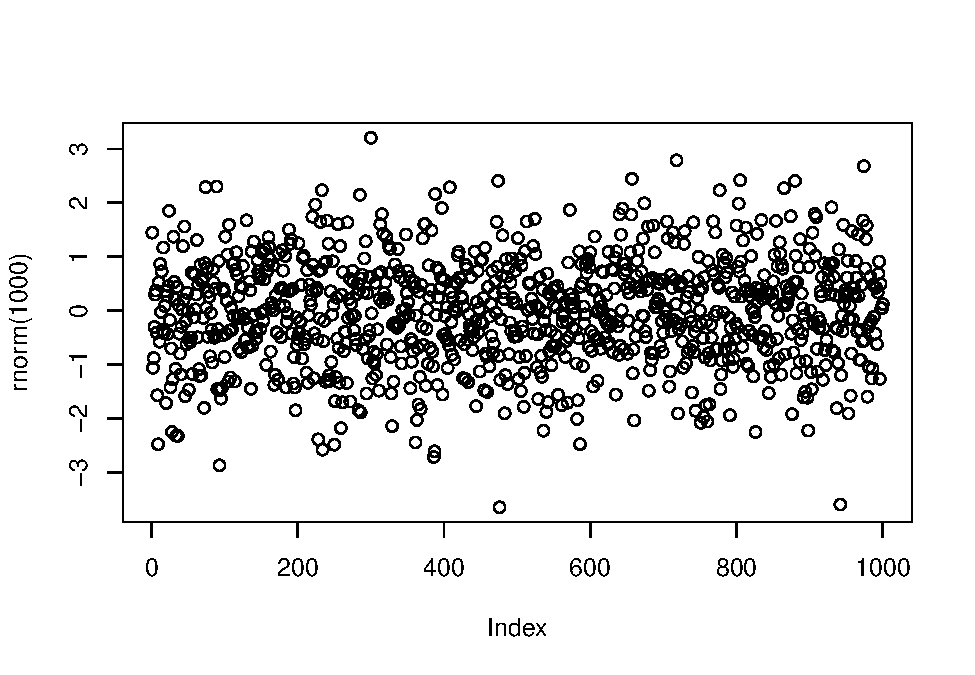
\includegraphics[width=1\linewidth]{d3book_files/figure-latex/unnamed-chunk-50-1}

\hypertarget{appendix-advanced-css}{%
\chapter{Appendix: advanced CSS}\label{appendix-advanced-css}}

\textbf{Work-in-progress}

\hypertarget{buttons}{%
\section{Buttons}\label{buttons}}

\hypertarget{active}{%
\subsection{\texorpdfstring{\texttt{.active}}{.active}}\label{active}}

This is a \emph{class} not a pseudoclass, indicates which button(s) are pressed.

\hypertarget{active-1}{%
\subsection{\texorpdfstring{\texttt{:active}}{:active}}\label{active-1}}

A pseudoclass. Clicking is the main way to trigger an \texttt{:active} state.

\hypertarget{focus}{%
\subsection{\texorpdfstring{\texttt{:focus}}{:focus}}\label{focus}}

A pseudoclass. Mainly used for tabbing. Clicking \emph{may} focus a button but \href{https://zellwk.com/blog/inconsistent-button-behavior/}{not always}. A box shadow such as \texttt{box-shadow:\ 0\ 0\ 0\ 3px\ lightskyblue;} is a \href{https://zellwk.com/blog/style-hover-focus-active-states/\#styling-focus-states}{good choice}

\hypertarget{hover}{%
\subsection{\texorpdfstring{\texttt{:hover}}{:hover}}\label{hover}}

As expected, can have separate hover behavior for \texttt{.active} buttons.

\hypertarget{example-2}{%
\subsection{Example}\label{example-2}}

{See the Pen
Button .active vs :active by Joyce Robbins (https://codepen.io/jtr13)
on CodePen.}

  \bibliography{book.bib,packages.bib}

\end{document}
